\documentclass[preprint,12pt,authoryear,a4paper]{elsarticle}
% Shared preamble of the manuscript and the supplementary material (elsarticle, XeLaTeX via tectonic).
\usepackage{fontspec}
\setmainfont{texgyretermes}[Extension=.otf,UprightFont=*-regular,BoldFont=*-bold,ItalicFont=*-italic,BoldItalicFont=*-bolditalic]
\setsansfont{texgyreheros}[Extension=.otf,UprightFont=*-regular,BoldFont=*-bold,ItalicFont=*-italic,BoldItalicFont=*-bolditalic]
\usepackage{amsmath}
\usepackage{unicode-math}
\setmathfont{texgyretermes-math.otf}
% a text block close to the journal's printed figure width (19 cm): figures print near their drawn size
\usepackage[a4paper,left=2.4cm,right=2.4cm,top=2.4cm,bottom=2.6cm,footskip=1cm]{geometry}
\usepackage{graphicx}
\graphicspath{{figures/}}
\usepackage{booktabs}
\usepackage{array}
\usepackage{tabularx}
\usepackage{longtable}
\usepackage{pdflscape}
\usepackage{rotating}
\usepackage{xcolor}
\usepackage{setspace}
\usepackage{lineno}
\usepackage[labelsep=period,labelfont=bf,font=small,justification=justified,singlelinecheck=false]{caption}
\usepackage{placeins}
\usepackage[hidelinks]{hyperref}
% citation links inside floats are misplaced by the PDF driver (xdvipdfmx): floats carry no links
\usepackage{etoolbox}
\AtBeginEnvironment{figure}{\NoHyper}
\AtBeginEnvironment{table}{\NoHyper}
\AtBeginEnvironment{sidewaystable}{\NoHyper}
% references as the journal prints them: DOIs as https://doi.org/..., no 'URL:' prefix, URLs in the text font
\urlstyle{same}
\providecommand{\DOIprefix}{}\renewcommand{\DOIprefix}{}
\providecommand{\URLprefix}{}\renewcommand{\URLprefix}{}
\providecommand{\doi}[1]{}\renewcommand{\doi}[1]{\url{https://doi.org/#1}}
\providecommand{\hy}{-}  % a hyphen that the bibliography style does not turn into a dash
\renewcommand{\figurename}{Fig.}
\newcolumntype{L}[1]{>{\raggedright\arraybackslash}p{#1}}
\newcolumntype{Y}{>{\raggedright\arraybackslash}X}
\newcolumntype{R}[1]{>{\raggedleft\arraybackslash}p{#1}}
\setlength{\tabcolsep}{4pt}
\setlength{\emergencystretch}{3em}  % fewer overfull lines in the justified text
% notes set below a table body
\newcommand{\tablenotes}[1]{\par\smallskip{\footnotesize\raggedright #1\par}}
\renewcommand{\thesection}{S\arabic{section}}
\renewcommand{\thefigure}{S\arabic{figure}}
\renewcommand{\thetable}{S\arabic{table}}
\renewcommand{\theequation}{S\arabic{equation}}
\begin{document}
\begin{center}
{\Large\bfseries Supplementary material}\\[2mm]
{\large Sensor noise, array design and helmet fit in on-scalp and cryogenic magnetoencephalography: a simulation study from adults to children}\\[2mm]
Laiba Khan and Mainak Jas
\end{center}
\linenumbers
\section{Estimands and conventions}\label{sec:S1}

We compared arrays of optically pumped magnetometers (OPMs) with the Neuromag magnetoencephalography (MEG) system of superconducting quantum interference devices (SQUIDs), by default all 306 of its channels. The primary metric is the known-topography detectability $d$ (main text, Section 2.1), the output signal-to-noise ratio (SNR) of the optimal matched filter, computed with the true (oracle) noise covariance and rank-aware whitening for every target and array. Arrays were compared target by target through the paired ratio $d_{\mathrm{OPM}}/d_{\mathrm{Neuromag}}$ or $D = 20\log_{10}(d_{\mathrm{OPM}}/d_{\mathrm{Neuromag}})$, which is positive when the OPM array is ahead and does not depend on the dipole moment. The adult comparison reports the median of the paired ratio, not the ratio of the two systems' median detectabilities.

The adult analyses use the unweighted median over all 7,661 targets, the 558 on the medial wall included. The smaller heads use an area-weighted median over cortical targets, medial wall excluded, because their cortices differ in size and their targets in density. At the adult's measured head position, the dense array's ratio is 1.144 unweighted over all targets, 1.148 without the medial wall and 1.158 area-weighted without it; its $D$ is +1.17~dB under the adult convention and +1.27~dB under the pediatric one. A 1\,\% change of the ratio is 0.086~dB, and 1~dB is a ratio of 1.122. Table~\ref{tab:S1} gives the adult's primary comparison in both forms.

\begin{table}[!htbp]
\caption{The adult's primary comparison as a ratio and in decibels. Median over all 7,661 targets of the paired ratio OPM/Neuromag (306 channels) and its $D$, with 95\,\% parcel-bootstrap intervals in brackets; the adult at its measured head position; OPM white noise 15~fT/√Hz.}\label{tab:S1}
\centering\footnotesize
\begin{tabularx}{\textwidth}{L{3.1cm}>{\centering\arraybackslash}X>{\centering\arraybackslash}X>{\centering\arraybackslash}X}
\toprule
Array and form & Sensor noise only & Sensor plus brain noise (primary) & Room field projected out \\
\midrule
Dense, ratio & 0.742 [0.717, 0.768] & 1.144 [1.121, 1.168] & 1.115 [1.081, 1.149] \\
Dense, $D$ (dB) & −2.59 [−2.89, −2.30] & +1.17 [+0.99, +1.35] & +0.95 [+0.68, +1.21] \\
Site-matched, ratio & 0.531 [0.512, 0.551] & 1.009 [0.994, 1.027] & 0.948 [0.899, 0.977] \\
Site-matched, $D$ (dB) & −5.50 [−5.82, −5.18] & +0.08 [−0.05, +0.23] & −0.46 [−0.92, −0.20] \\
\bottomrule
\end{tabularx}
\tablenotes{Dense, the dense OPM array; site-matched, the site-matched OPM array; $D = 20\log_{10}$ of the ratio.}
\end{table}

Every $\Delta$ is taken against the adult placed by the same rule, because the adult's own $D$ depends on the placement. It is +1.27~dB at its measured head position, +1.00~dB at top contact, +1.01~dB laterally centered and raised to contact and +0.87~dB at true contact. In its own helmets scaled with the head it is +1.27 and +1.28~dB (centered and laterally centered; scale factor 1.000), and in the helmet fitted at its own gap +1.28~dB. $\Delta$ is reported descriptively, without a test or a margin; where a difference of two pooled medians replaces it, the text says so.

Peak-channel SNR divides each channel by its own noise, so magnetometers and gradiometers compete on equal terms. It is the closest analogue of the sensor-level SNRs of the clinical studies, except that a clinical baseline standard deviation also holds physiological noise, whereas the model's holds only what the noise model contains. Mean-power SNR is the channel-averaged SNR of \citet{goldenholz2009}, also used by \citet{matsubara2026}.

The plug-in filter is built from a Ledoit--Wolf covariance estimate \citep{ledoit2004} and evaluated under the true covariance, so it cannot exceed the oracle value. The estimate from 4,680 samples is the declared 60-s scenario; its samples are independent, which does not establish the effective sample size of a measured colored-noise baseline. The estimate from 780 samples shows how a short baseline penalizes the array with more channels.

Neighboring cortical targets are correlated, so no interval resamples targets as if they were independent, except in the adult's frequency-band comparison, whose intervals are therefore narrower than those of the primary comparison. All intervals are percentile intervals; in the spike study the location is the statistical unit (Section~\ref{sec:S7}). Table~\ref{tab:S16} gives the resample count of every interval family, and Table~\ref{tab:S2} lists every estimand of the study, its definition, its interval and what that interval covers.

\FloatBarrier
{\scriptsize
\setlength{\LTcapwidth}{\textwidth}
\begin{longtable}{@{}L{2.2cm}L{8.0cm}L{3.4cm}L{1.6cm}@{}}
\caption{Estimands of the study in full.}\label{tab:S2}\\
\toprule
Estimand & Definition & Interval and what it covers & Used in (section) \\
\midrule
\endfirsthead
\multicolumn{4}{@{}l}{\small\textbf{Table~\thetable.} Estimands of the study in full (continued).}\\[2pt]
\toprule
Estimand & Definition & Interval and what it covers & Used in (section) \\
\midrule
\endhead
\midrule
\multicolumn{4}{r@{}}{(continued on next page)}\\
\endfoot
\bottomrule
\endlastfoot
Adult ratio & Median over all 7,661 targets (medial wall included) of the paired ratio $d_{\mathrm{OPM}}/d_{\mathrm{Neuromag}}$, or $D$; conditions: sensor noise only, sensor plus brain noise (primary), with the room field, projected & 95\,\% bootstrap over the adult's 70 labels (atlas parcels and the two medial-wall labels) & 3.1--3.3; \ref{sec:S2}, \ref{sec:S3} \\
Scenario ratio & The adult ratio with sensor, brain and room noise (Neuromag's 305 good channels) under one of five stated assumptions about how each system's real noise departs from the model, informed by Neuromag's measured covariance (scenarios A--E) & Parcel bootstrap over the same labels & 3.2; \ref{sec:S3} \\
Break-even noise & The OPM white-noise level at which the adult ratio equals 1, found on a grid of 33 levels over 4–60~fT/√Hz & Parcel bootstrap of the crossing & 3.1, 3.2; \ref{sec:S3} \\
Depth-bin ratio & Median of the paired ratio over the targets of one 5-mm depth bin & Bootstrap over the parcel labels present in the bin & 3.3 \\
Regional ratio & Median of the paired ratio over a lobe's or a parcel's targets & Lobes: bootstrap over the lobe's parcels; single parcels: the interquartile range over targets, a spread rather than a confidence interval & 3.3 \\
$D$ of a head & Area-weighted median of $D$ over a head's cortical targets, medial wall excluded, in a named helmet and placement & Parcel bootstrap within the head & 3.4, 3.5; \ref{sec:S5}, \ref{sec:S6} \\
$\Delta$ & $D_{\mathrm{head}} - D_{\mathrm{adult}}$, the adult placed by the same helmet rule: vertex-wise for the scaled adults (the same cortical vertex); for the templates and children, which have no vertex correspondence, the adult-area-weighted median of parcel-level differences & Parcel bootstrap & 3.4, 3.5; \ref{sec:S5} \\
$\Delta$ within a depth stratum & The difference of the two heads' area-weighted medians within one stratum of depth below each head's own scalp (edges at 0, 10, 15, 20, 25, 30, 40, 50, 60, 90~mm), for every head including the scaled adults; strata with fewer than 10 targets in either head are not summarized & Parcels resampled in each head independently & 3.6; \ref{sec:S5} \\
Depth-reweighted difference & The difference of pooled medians after weighting each head's targets to the adult's depth distribution; not the same estimand as $\Delta$ & None (point estimate) & \ref{sec:S5} \\
Within-head contrast & The area-weighted median over one head's targets of the target-wise difference $D$(fixed helmet at top contact) $-$ $D$(fitted helmet), not the difference of the two medians; the OPM array is the same in both, so it is a property of Neuromag alone & Parcel bootstrap & 3.5; \ref{sec:S5} \\
Interaction & The within-head contrast of the smaller head minus that of the adult; at every vertex of a scaled adult it equals $\Delta$(fixed) $-$ $\Delta$(fitted), but the area-weighted medians are not additive & Parcel bootstrap & 3.5, 4.2, 4.4, 5; \ref{sec:S5} \\
$\Delta$ at equal OPM site count & $\Delta$ with the adult's dense array subsampled by farthest-point sampling to the smaller head's dense site count, the adult in the same helmet rule & Parcel bootstrap & 3.5; \ref{sec:S5} \\
Placement band & $\Delta$ at each of the 12 source-blind placements of the fixed helmet (each head against the adult at the same placement), as a difference of area-weighted medians; the crossed band pairs any feasible placement of the head with any of the adult & The range over placements, no interval & 3.4; \ref{sec:S5} \\
Peak-channel SNR & Each system's largest ratio of a channel's noise-free signal to that channel's own in-band noise standard deviation; OPM over Neuromag (best of all channels, or of the magnetometers) & Parcel bootstrap (adult); medians only (smaller heads) & 3.1, 4.1, 4.3; \ref{sec:S2}, \ref{sec:S3}, \ref{sec:S6} \\
Mean-power SNR & $10\log_{10}$ of the channel mean of the squared SNRs \citep{goldenholz2009}, compared as an amplitude ratio & Parcel bootstrap & 3.1 \\
Plug-in detectability & The output SNR under the true covariance of the matched filter built from a Ledoit--Wolf estimate from 780 or 4,680 independent samples (twice the time-bandwidth product of 10 and 60~s in this band), drawn for all arrays from one common noise realization & Parcel bootstrap & 3.1; \ref{sec:S3} \\
S50 & The strength at which a depth band's focal detection rate reaches 50\,\%, interpolated linearly in log strength; the band's locations (18 per band in the exploratory run, 36 in the pre-specified run) and 3 morphologies are pooled & Bootstrap over locations (1,000 resamples); open at one end when resamples do not reach half detection within the tested strengths & 3.6; \ref{sec:S7} \\
Paired S50 ratio & S50\textsubscript{Neuromag}/S50\textsubscript{OPM}, a ratio of the two pooled S50 estimates, above 1 when the OPM needs less strength; each bootstrap resample draws locations with replacement and recomputes both S50 values on them, so the ratio is paired by location, not a median of location-specific ratios & Location bootstrap, as S50 & 3.6; \ref{sec:S7} \\
Detection-count difference & Per location, the number of events detected by one array minus the other, tested with the two-sided sign-flip test over locations; every p-value reported is exact over all sign patterns & None; a p-value & 3.6; \ref{sec:S7} \\
Localization error & Distance from the true source (a patch's center) to the fitted dipole or to the dSPM peak, read at the true peak sample through the perturbed transform & Paired differences: bootstrap over events; Wilcoxon signed-rank p-value & 3.6; \ref{sec:S7} \\
Joint success & Detection by the practical detector with a localization error of at most 10~mm; paired differences tested with an exact McNemar test & None; a p-value & \ref{sec:S7} \\
\end{longtable}
}
\vspace{-\baselineskip}
\tablenotes{$d$, known-topography detectability with the oracle covariance; $D = 20\log_{10}(d_{\mathrm{OPM}}/d_{\mathrm{Neuromag}})$; Neuromag, all 306 channels unless stated. Every parcel bootstrap is a percentile interval over the parcels of one anatomy; it describes spatial variation within that anatomy and excludes placement, construction and between-subject variability. Sections 3.1--5 are in the main text, Sections S2--S7 in this supplementary material. dSPM, dynamic statistical parametric mapping \citep{dale2000}; SNR, signal-to-noise ratio.}

\section{The spherical benchmark}\label{sec:S2}

We reimplemented the analytical model of \citet{jas2026}: a tangential current dipole of 30~nAm in a spherical conductor (head radius 95~mm, brain radius 80~mm), with point magnetometers measuring the radial field on the scalp (OPM) and 18~mm above it (SQUID). The single-channel signal-to-noise ratio (SNR) is the peak field over the noise standard deviation $\sigma$, with $\sigma_{\mathrm{OPM}} = \eta\,\sigma_{\mathrm{SQUID}}$; the equal-SNR depth is the exact root of the preprint's Eq.~3. We checked the peak field against the full Sarvas field maximized over the sensor sphere (largest relative difference 4.7 $\times 10^{-15}$) and against the sphere model of MNE-Python \citep[5.4 $\times 10^{-8}$;][]{gramfort2013}.

The reimplementation reproduced the preprint (Fig.~\ref{fig:S1}A). At $\eta$~=~3 the exact equal-SNR depth is 27.665~mm; the preprint prints 28~mm and draws 27.53~mm, a difference of rounding and grid, not of model. A crossing exists only for $\eta$ between 1.683 and 5.309 (printed as 1.7 and 5.3). Only $\eta$ enters the equal-SNR depth: scaling both noises together leaves it at 27.665~mm.

On the real head, the ratio of the peak field at the best OPM to that at the best Neuromag magnetometer falls with depth as the sphere predicts once the sphere is given the real median standoffs (7.0~mm for the OPMs, 29.8~mm for the magnetometers). For the dense array it fell from 5.41 in the 10–15~mm bin to 2.28 at 55–60~mm, against 5.26 and 2.09 for the sphere.

To bridge the two models we used the sphere's own metric, peak-channel SNR against the magnetometers with sensor noise only, a single-channel quantity rather than the primary endpoint. At $\eta$~=~3 the realistic equal-SNR depth was 29.6~mm (site-matched array) and 31.8~mm (dense array), against 29.0~mm for the sphere with the real standoffs. For $\eta$ from 2.5 to 4.5, the arrays' depths lay within −0.8 to +5.4~mm of the sphere's (Fig.~\ref{fig:S1}B).

Outside that window the models differed. The OPMs were ahead at every depth for $\eta \le$ 2.25, where the sphere still predicts a deep crossing (48.8~mm), because the real peak-field ratio levels off at depth (2.35 at 60–65~mm) while the sphere's keeps falling (2.02). Neuromag's magnetometers were ahead at every depth for $\eta \ge$ 5.0 (site-matched) or 5.5 (dense). The sphere is therefore right about the geometry of magnetometers near its reference $\eta$. Against Neuromag's 204 planar gradiometers, the ratio with sensor noise only barely changed with depth, so the sphere describes only the magnetometer part of the comparison; $\eta$ itself is left to the explicit noise model (Section~\ref{sec:S3}).

For head size, we placed the preprint's newborn, 1-year, 8-year and adult spheres in a SQUID shell that follows each head at 18~mm, as in the preprint, and, as a contrast, in the adult shell of radius 113~mm. With the size-following shell, the equal-SNR depth at $\eta$~=~3 hardly moved from adult to newborn (27.7–30.8~mm), but the normalized depth rose from 15.8\,\% to 49.6\,\%, because the brain and the extracerebral layer (7–15~mm in the preprint's heads) shrink. In the single adult shell, size and fit are confounded: the OPM was ahead at every depth of the newborn and 1-year brains up to $\eta$~=~8.7 and 4.2, respectively. The sphere's prediction for children thus assumes a shell that follows the head at a constant gap.

\begin{figure}[tbp]
\centering
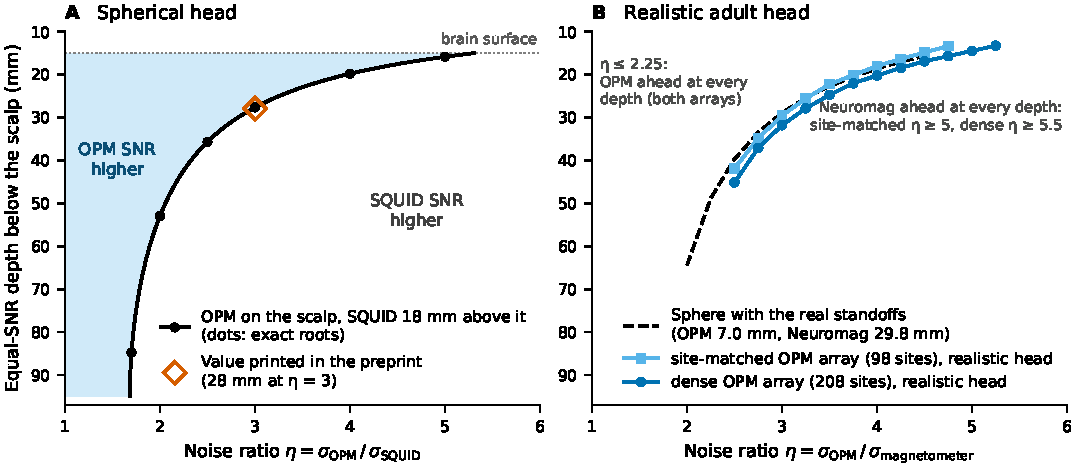
\includegraphics[width=\textwidth]{Figure_S1.pdf}
\caption{The spherical benchmark and its transfer to a real head. (A) The spherical head of \citet{jas2026}, reimplemented: equal-SNR depth below the scalp against the noise ratio $\eta = \sigma_{\mathrm{OPM}}/\sigma_{\mathrm{SQUID}}$ for a point magnetometer on the scalp (OPM) and one 18~mm above it (SQUID). Dots, exact roots at selected noise ratios; diamond, the preprint's printed value (28~mm at $\eta$~=~3); dotted line, the brain surface (15~mm below the scalp); shaded, the OPM's single-channel SNR is higher. Adapted from \citet{jas2026}, Fig.~4E (CC BY 4.0, \url{https://creativecommons.org/licenses/by/4.0/}), redrawn from our reimplementation of their model. (B) The same on the realistic adult head with peak-channel SNR against the Neuromag magnetometers and sensor noise only, for the site-matched (98 sites, squares) and dense (208 sites, circles) arrays, drawn at the noise ratios at which each array has a crossing; dashed, the sphere at the real median standoffs. SNR, signal-to-noise ratio; OPM, optically pumped magnetometer; SQUID, superconducting quantum interference device.}
\label{fig:S1}
\end{figure}

\section{The noise model: components, calibration, validation and sensitivity analyses}\label{sec:S3}

\subsection{Components and calibration}\label{sec:S3.1}

Every array saw the same noise sources in the 1–40~Hz band (zero-phase Butterworth filter of order 4; equivalent noise bandwidth 35.1~Hz), and its oracle covariance was computed in closed form (main text, Eq.~(3)), each diagonal sensor-noise entry being a channel's squared spectral density times the equivalent noise bandwidth. We chose this band because the matched filter's gain rests on the lower frequencies, where the brain noise sits.

The OPM sensor noise, 15~fT/√Hz in the primary analysis and swept over 7–30~fT/√Hz, is a declared parameter, not a measured device value. It lies within the sensor noise quoted by the clinical OPM studies, although those studies state no band and the device specifications behind them begin at 1~Hz or above \citep{osborne2018}. The top of the sweep is close to the empty-room floor of the recording of \citet{jas2026}, read from its Fig.~9 on the assumption that its unstated dB reference is 1~fT²/Hz. The Neuromag values, the TRIUX datasheet's typical values (main text, Section 2.3), describe a representative system rather than one installation; in the band they amount to 20.7~fT and 21.3~fT/cm root-mean-square (RMS). Noise from the measured empty-room spectrum (25.9~fT, 20.0~fT/cm) is a sensitivity analysis. The Neuromag coils are integrated over 8 points per gradiometer and 16 per magnetometer.

The 1,755 background dipoles are a greedy Poisson-disk subset of the usable white-surface vertices with 7-mm minimum spacing (seed 2026), and their Voronoi cells partition the 1,878~cm² of usable cortex (107~mm² on average). Source $i$'s moment variance is $\sigma^{2} a_i$, $a_i$ being its cell area, a standard deviation of 0.188~nAm~×~√($a_i$/mm²), or 1.95~nAm RMS over the sources; $\sigma^{2}$ was fitted once and kept per unit area on every head. The excluded cortex within 4~mm of the inner skull (8.7\,\% of the vertices) holds the sources nearest to every sensor; Section~\ref{sec:S3.6} adds it back. Spatially correlated variants used correlation lengths of 5 and 10~mm.

The measured brain noise, to which $\sigma^{2}$ was calibrated on the median good gradiometer, is the in-band variance of the 320 pre-stimulus windows of the sample recording minus that of its empty-room recording, the bad channel excluded. The windows begin soon after the previous stimulus, so they hold task-related rather than only resting activity. The 8 room-field terms (about (0, 0, 40)~mm in the head frame) pass through each array's own coil integration points, and their covariance was fitted to the band-filtered empty-room recording. Plug-in covariances are Ledoit--Wolf estimates from 780 or 4,680 independent samples, twice the time-bandwidth product of 10 and 60~s.

The room field is removed by the projection
\begin{equation}
P = I - E\left(E^{\mathsf{T}} W E\right)^{-1} E^{\mathsf{T}} W,
\label{eq:S-projection}
\end{equation}
where $E$ holds the array's responses to the room-field terms and $W$ is the inverse of the diagonal sensor-noise covariance. It is applied to topographies $s$ and covariance $C$ alike ($Ps$, $PCP^{\mathsf{T}}$), by the same rule for every array. For Neuromag it acts on all 306 channels jointly, so its magnetometer and gradiometer comparisons after projection use subsets of jointly projected data. The retained ranks were 298 of 306 for Neuromag (99 of 102 magnetometers, 204 of 204 gradiometers), 200 of 208 for the dense array and 90 of 98 for the site-matched array. Whitening drops eigenvalues of the correlation-normalized covariance below $10^{-10}$ of the largest. Relative to the room field without projection, the projection cost Neuromag 0.48\,\% of its detectability, the dense array 2.5\,\% and the site-matched array 6.0\,\%.

The OPM sensitive axes were computed from the triangles of the boundary-element model (BEM) head surface on the magnetic resonance imaging (MRI) scalp. They deviated from a plane fitted to the dense MRI scalp by a median 1.2° (95th percentile 4.9° site-matched, 7.4° dense). The adult's stored outer-skin normals lie within 5° of the radial direction. With those axes at the same sites, the projected dense ratio was 1.073 [1.017, 1.115] instead of 1.115, and 0.82 instead of 0.98 at 45--70~mm: nearly radial axes make room-field patterns resemble those of deep sources, so the projection removes more of their signal. Without projection, the two constructions gave 1.130 against 1.144.

In the band sensitivity analysis, the brain scale and room field were refitted per band, with and without a first-order 100-Hz OPM response. The dense ratio with sensor plus brain noise was 1.15 at 1–10~Hz, 1.14 at 8–30~Hz and 1.11 at 30–80~Hz (1.07 with the OPM response), against 1.14 in the analysis band; the site-matched ratio was 1.00, 1.01 and 0.99. Sensor noise was 1.3\,\% and 23\,\% of a dense-array channel's variance at 1–10 and 30–80~Hz, and 9.3\,\% and 74\,\% of a Neuromag channel's.

In a 3–70~Hz band, typical of clinical spike review, the dense ratio was 1.137 (1.130 with the OPM response) and the site-matched ratio 1.011, against 1.144 and 1.009 in the analysis band. Their target-bootstrap intervals, [1.133, 1.141] and [1.009, 1.013], are narrower than the parcel bootstrap of the primary comparison (Section~\ref{sec:S1}). Projected, the two ratios were 1.108 and 0.945. Sensor noise was 5.6\,\% of a dense-array channel's variance in this band and 34\,\% of a Neuromag channel's.

\subsection{What is fitted, calibrated, checked and predicted}\label{sec:S3.2}

Four kinds of agreement must be kept apart (Fig.~\ref{fig:S2}B). For the magnetometers, the room field was fitted to the empty-room recording; with the datasheet sensor noise it reproduced their empty-room level (114.9 against 115.2~fT measured) and explained 94\,\% of their empty-room variance. For the gradiometers it explained only 1.6\,\%, so their empty-room agreement (21.4 against 20.2~fT/cm measured) is an independent check of the datasheet's sensor noise against this one recording, whose level the model slightly exceeds. The gradiometer brain noise is calibrated: 37.1~fT/cm, equal to the measurement by construction.

The magnetometer brain noise, the one independent prediction of the background's median level, fell short: 192~fT modeled against 262~fT measured (0.73 times). The measured value also holds non-cortical physiological fields that the model omits by design, so the shortfall is not purely an error of the cortical background; Section~\ref{sec:S3.4} separates the heart's part. No OPM noise was measured: its sensor noise is declared, and its brain and room noise are the Neuromag-calibrated model seen through the OPM arrays' lead fields.

Two published simulation studies, each adapted with its own design, check shape and level. Our adaptation of the depth-orientation maps of \citet{hunold2016} correlated with the published dipole maps at r~=~0.96–0.98 but reached only 0.74–0.79 times their level (patch maps: r~=~0.93–0.94, 0.79–0.85 times), even with a background scale fitted to the paper's example traces. The calibration rule of \citet{goldenholz2009} gave a noise-source amplitude within their published range once normalized to their number of sources (1.77 against 1.6–1.9~nAm; 2.68~nAm on our grid). The first used 600-nAm spike-wave sources over randomly placed cortical dipoles, conductivities of 0.33, 0.0042, 0.33~S/m and peak-to-peak signal-to-noise ratio (SNR); the second, 10-nAm dipoles, channel-averaged power SNR and a background calibrated on recorded noise.

Both show the dependence on metric examined in the main text. With brain noise only, the best single channel of a site-matched OPM array in the first reached only 0.70–0.84 times the SNR of the planar gradiometers in every depth row, and 0.89–1.37 times that of the magnetometers, falling with depth. With the channel-averaged SNR of the second, the OPM was within about 0.1~dB of both (−0.08~dB against the gradiometers, +0.09~dB against the magnetometers).

In this model, brain noise dominates both kinds of magnetometer channel: 92\,\% of a dense-array OPM channel's in-band variance (room field 4.9\,\%, sensor noise 3.0\,\%) and 74\,\% of a Neuromag magnetometer's (room field 25\,\%, sensor noise 0.9\,\%), whereas sensor noise was 25\,\% of a gradiometer's (Fig.~\ref{fig:S2}A, C).

The implied single-channel noise ratio OPM/magnetometer, the analogue of $\eta$, was about 2.6 with sensor plus brain noise, the primary condition (2.3 with the room field added). In the recording of \citet{jas2026} it is about 4.6, over a much wider band (4–330~Hz). Approximate readings of its spectra, not results of this study, locate the difference: where brain activity dominates, the OPM/SQUID ratio of the spectral peaks is about 2.0, but the measured OPM has an empty-room floor of about 28–35~fT/√Hz and a distance-independent low-frequency component of about 200–224~fT/√Hz at its peak. The model thus lacks the OPM's own floor and a non-brain low-frequency component, which would explain why the measured OPM noise barely fell when the sensors were lifted. Both readings of the preprint's Fig.~9 are uncertain, and the preprint (version 1) has not been peer reviewed.

\begin{figure}[tbp]
\centering
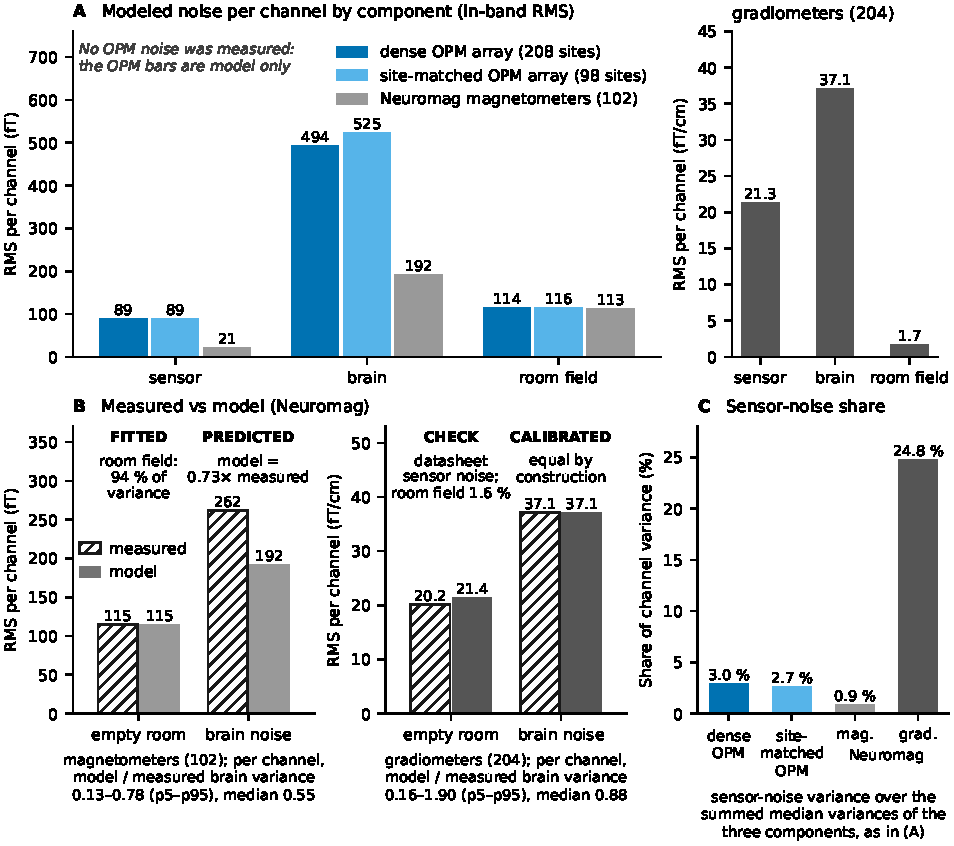
\includegraphics[width=\textwidth,height=0.5\textheight,keepaspectratio]{Figure_S2.pdf}
\caption{The noise budget and what is fitted, checked, calibrated and predicted. (A) Modeled in-band RMS noise per channel by component (sensor noise, cortical background, room field), the square root of each component's median channel variance (RMS values do not add), for the dense OPM array (208 sites), the site-matched OPM array (98 sites) and Neuromag's 102 magnetometers; the 204 gradiometers on their own fT/cm axis. The OPM bars are model only. (B) Measured Neuromag quantities against the model: the empty-room level (magnetometers, a fit; gradiometers, a check) and the brain noise (magnetometers, a prediction; gradiometers, calibrated). Labels under the panels give the median and the 5th to 95th percentiles over channels of the modeled-to-measured brain-noise variance; the covariance check of Section~\ref{sec:S3.4} excludes the bad channel, so its gradiometer range differs slightly. (C) The sensor-noise share of the in-band variance with brain noise and room field. RMS, root-mean-square.}
\label{fig:S2}
\end{figure}

\subsection{Why the ratio falls with depth, and the other adult conditions}\label{sec:S3.3}

Against Neuromag's 306 channels, the dense ratio fell with depth even with sensor noise alone, from 1.00 to 0.64. Neuromag's detectability with sensor noise only rests on its magnetometers, and the peak-field ratio OPM/magnetometer fell from 5.41 in the shallowest bin to 2.28 at 55–60~mm. The detectability ratio, drawing on many channels, fell less steeply.

Against the 204 gradiometers alone, the ratio with sensor noise only barely changed with depth (3.56 at 10–15~mm, 3.08 at 20–25~mm, 3.44 at 60–65~mm). With brain noise it fell from 1.88 to 1.17 at 35–40~mm: here the depth dependence comes from brain noise, which costs every array most for deep sources.

Adding brain noise multiplied the dense ratio by a nearly constant factor in every depth bin (main text, Section 3.3); for the site-matched array the factor rose with depth (1.69–2.09) and partly offset the geometric fall. The factor follows the per-channel noise budget, not better whitening by the denser array: brain noise multiplied the in-band noise of a Neuromag magnetometer about 9.3-fold over its sensor floor but that of an OPM only about 5.7-fold (a ratio of 1.65), and the sparser site-matched array had the larger factor.

With sensor plus brain noise, the dense array was behind Neuromag at 4 of the 7,661 targets, on the left medial orbitofrontal (3) and left medial wall (1), 26.5–35.1~mm below the scalp (ratios 0.956–0.997). Pooled over both hemispheres, 12 atlas parcels had a smaller dense lead than the parahippocampal cortex (1.12): posterior cingulate (1.03), precuneus (1.05), caudal anterior cingulate (1.05), transverse temporal (1.06), lingual (1.06), pericalcarine (1.06), paracentral (1.07), rostral anterior cingulate (1.07), isthmus cingulate (1.07), insula (1.09), medial orbitofrontal (1.12) and banks of the superior temporal sulcus (1.12).

A covariance estimated from 780 samples cost Neuromag more than the OPMs (15\,\% of the oracle detectability, against 9.1\,\% for the dense and 5.1\,\% for the site-matched array), raising the dense ratio to 1.23 and the site-matched ratio to 1.12. With 4,680 samples, the declared 60-s scenario, the penalty was small for every array (main text, Fig.~3). The site-matched array's interval lay above 1 at an OPM white noise of 10~fT/√Hz (1.049 [1.032, 1.068]) and below 1 at 20~fT/√Hz (0.983 [0.967, 0.997]).

Three axes with equal noise at the 98 site-matched sites (294 channels) raised the ratio from 1.01 to 1.12 (1.17 projected), close to the dense array's 1.14 from 208 single-axis sites; with tangential axes twice as noisy it was 1.05.

\subsection{The model against the measured Neuromag covariance}\label{sec:S3.4}

The measured brain-noise covariance leaves out the bad channel (MEG 2443) and has no signal-space projection, as in the adult comparison, leaving 305 channels (102 magnetometers, 203 gradiometers). Only the background's scalar and the room field's 8~×~8 coefficient covariance are fitted to this dataset; everything below is an independent prediction.

Comparisons of a sample covariance with an exact one are calibrated on surrogates: phase-randomized records recolored to the model, with the same number of samples, give the range an exact model would show when ``measured'' the same way, so a value outside it is a real departure from the model.

The model predicted the magnetometers' median brain-noise amplitude at 0.73 of the measured; an exact model would give 0.98–1.03. For the gradiometers, the scale fitted on half the sites predicted the other half's median amplitude to 1.00 [0.93, 1.09] over 1,000 random halves (Fig.~\ref{fig:S3}B). Fitted on the inferior half, it predicted the superior half to 1.34, and the other way round to 0.75: the modeled brain noise is too flat from bottom to top.

The per-channel pattern was poorly predicted (Fig.~\ref{fig:S3}A, C): the Pearson correlation of model and measured log variances was 0.14 for the magnetometers and 0.43 for the gradiometers, against a split-half reliability of the measurement of 0.93 and 0.97. The model/measured variance spanned 0.13–0.78 over the magnetometers (5th to 95th percentile) and 0.19–1.90 for the gradiometers, where an exact model would give about 0.95–1.06. The correlation matrices agreed better (r~=~0.88 for the magnetometers, 0.76 for the gradiometers).

Against inter-sensor distance, the modeled magnetometer correlations followed the measured ones at 25–50~mm (0.85 against 0.90) and fell faster beyond, to −0.30 against 0.00 at 200–225~mm (Fig.~\ref{fig:S3}D). Spatially correlated backgrounds did not change this, because the measured long-range correlation is a far-field pattern, not a cortical one. The gradiometers' median signed correlations agreed at every distance (0.36 against 0.34 at 25–50~mm; Fig.~\ref{fig:S3}E).

The measured magnetometer brain noise is more concentrated than the model's (Fig.~\ref{fig:S3}G, H). Its leading five components held 82\,\% of the variance against 72\,\% in the model (participation ratio 5.5 against 7.4), whereas the gradiometer spectra agreed (49\,\% against 48\,\%). The magnetometers' excess over the model was itself concentrated (91\,\% in three components), and 91\,\% of its leading component lay in the 8-dimensional far-field subspace of the room-field terms, against 7.8\,\% for a random direction.

A cardiac-locked average over 282 beats (heart rate 62 per minute) added 127~fT RMS to the median magnetometer's baseline windows: 25\,\% of the measured magnetometer brain variance and 51\,\% of the model's shortfall, its leading component lying 91\,\% in the far-field subspace. With the heart's field removed, the magnetometer prediction was 0.89 of the measured amplitude, and the correlation of the log variances rose to 0.76 (magnetometers) and 0.66 (gradiometers). The heart thus explains about half of the shortfall and much of the pattern error; the rest lies in far-field components, consistent with distant or non-cortical sources, or with cortical activity correlated over longer distances than the 5 and 10~mm tested.

With the background scale refitted per band on the gradiometers, the magnetometer prediction fell with frequency, from 0.97 at 1–4~Hz to 0.33 at 30–40~Hz (Fig.~\ref{fig:S4}C), and the measured magnetometer excess over the gradiometer-calibrated model grew from 1.07 to 9.28 in variance over the same bands. The six sub-band variances sum to 0.98 (magnetometers) and 0.95 (gradiometers) of the whole-band baseline variance. The magnetometers' empty-room level was predicted to 0.75 at 1–4~Hz and 0.98–1.01 from 8–13~Hz up.

Detectability with a sample covariance is biased upward by the finite number of samples; the bias, computed on the surrogates, was 1.03 for the 305 channels, and every ratio below is divided by it target by target. Uncorrected, Neuromag's detectability with the measured covariance was 1.18 [1.12, 1.24] times its modeled value; corrected, it was 1.14 [1.08, 1.20], where an exact model measured the same way gives about 1. The magnetometers alone gave 1.059 [1.003, 1.119] and the gradiometers 1.12 [1.07, 1.18]. With the heart's field removed, the ratio was 1.15. With the measured empty room and the modeled brain noise it was 1.01: the departure comes from the brain noise, not the room.

By lobe, the measured-over-modeled ratio was 1.40 for the cingulate, 1.25 frontal, 1.06 insula, 1.07 occipital, 1.19 parietal and 0.89 temporal. By depth, the median ratio was 1.19 at 10–15~mm, lowest (1.09) at 40–45~mm and highest (1.42) at 60–65~mm. The real noise thus favors Neuromag more than the modeled noise, most for deep and cingulate sources, because the measured excess is concentrated in a few far-field components that the whitening removes at little cost.

\begin{figure}[p]
\centering\captionsetup{font=footnotesize}
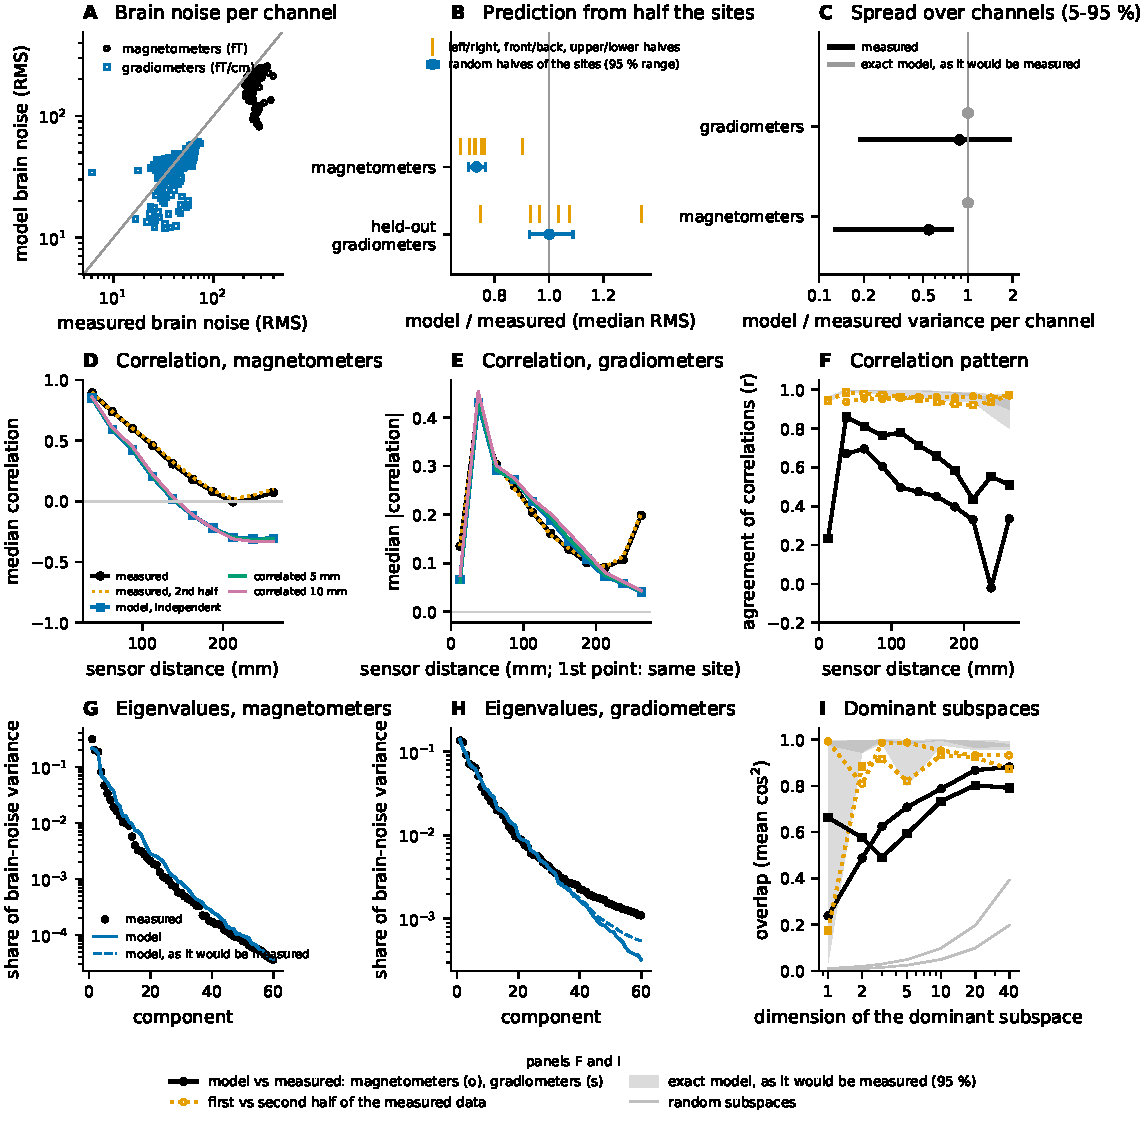
\includegraphics[width=\textwidth]{Figure_S3.pdf}
\caption{Structure of the measured and modeled Neuromag brain noise (task baseline minus empty room, 1–40~Hz). (A) Modeled against measured RMS brain noise per channel (magnetometers, fT; gradiometers, fT/cm; logarithmic axes; diagonal, equality). (B) Model over measured median amplitude, scale fitted on half the sites: random halves (1,000 splits; dot and 95\,\% range) and six directional halves (ticks: left and right, front and back, upper and lower), for the magnetometers and the held-out gradiometers. (C) The 5th to 95th percentile over channels of the modeled-to-measured variance (black) and the exact-model range (gray). (D) Median correlation between magnetometers against distance: measured (both halves of the recording), the model with independent background sources and with correlation lengths of 5 and 10~mm. (E) The same for the gradiometers as the median absolute correlation; the first point is the two gradiometers of one site. (F) Agreement of the correlation patterns per distance bin (Pearson r over channel pairs): model against measurement (black; circles, magnetometers; squares, gradiometers), the two halves of the measurement (orange, dotted) and the exact-model band (gray). (G, H) Eigenvalue spectra as shares of the variance: measured (dots), model (line) and model as measured (dashed). (I) Overlap (mean squared cosine) of the dominant subspaces of model and measurement against subspace dimension, with the two halves of the measurement (orange), the exact-model band (gray) and random subspaces (thin gray lines). Exact-model ranges and bands come from surrogates measured like the recording. RMS, root-mean-square.}
\label{fig:S3}
\end{figure}

\begin{figure}[tbp]
\centering
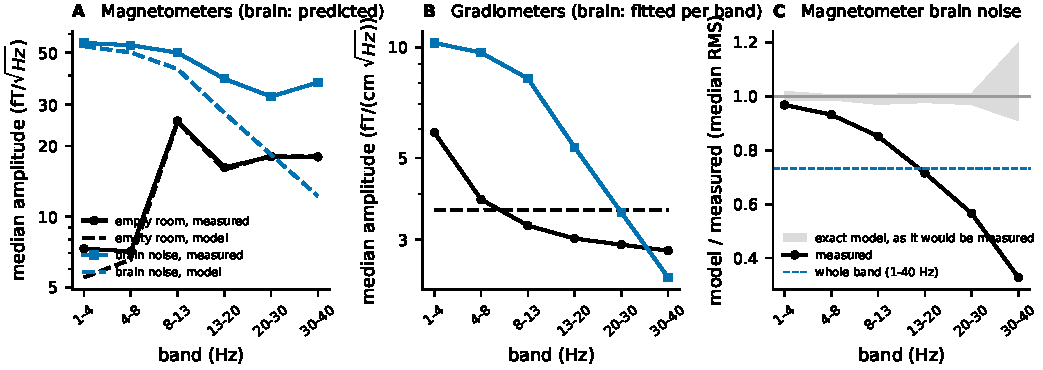
\includegraphics[width=\textwidth]{Figure_S4.pdf}
\caption{The prediction by sub-band (1–4, 4–8, 8–13, 13–20, 20–30 and 30–40~Hz; background rescaled in each band on the gradiometers). (A) Magnetometers: median amplitude spectral density of the measured and modeled empty room (black) and brain noise (blue, the prediction). (B) Gradiometers: the measured brain noise and the model fitted to it per band (blue); the measured empty room and the model's band-independent sensor noise (black). (C) The magnetometer brain-noise prediction per band, model over measured median RMS. Dashed, the whole-band value; gray, the exact-model range. RMS, root-mean-square.}
\label{fig:S4}
\end{figure}

\subsection{Scenarios A--E: what the check implies for the OPM}\label{sec:S3.5}

Because the OPM's covariance cannot be measured here, Table~\ref{tab:S3} gives the implied OPM/Neuromag ratio under five stated assumptions about its real noise (main text, Section 3.2), with sensor, brain and room noise, like for like with the measured covariance. In scenario A, the OPM's real covariance changes its detectability, target by target, by the same factor as the measured covariance changes Neuromag's, so the ratio is the model's own. In B, both cortical backgrounds are scaled by $k$ with the model's structure kept. In C, the OPM bears the whole excess as cortical noise and none of its measured structure. In D, the model's error is specific to Neuromag. E, with Neuromag's measured empty room and modeled brain noise and the OPM as modeled, isolates the sensor and room part of Neuromag's noise.

Scenarios A, B and E left the primary model's ratios nearly unchanged. Scenario D left the dense array with no established advantage and the site-matched array below 1. By depth, scenario D left the dense array's median at 1.35 and 1.20 in the 10–15 and 15–20~mm bins and below 1 from the 25–30~mm bin on (point estimates over the per-target values, room field included). Scenario C put both arrays well below 1. Which scenario holds depends on how the OPM's real noise departs from the model, which no measurement here constrains; the noise model is validated in part for Neuromag, not for the OPM arrays.

\begin{table}[tbp]
\caption{The implied OPM/Neuromag ratio under scenarios A--E. Median over the 7,661 targets; sensor, brain and room noise, unprojected; Neuromag's 305 good channels; 95\,\% parcel-bootstrap intervals in brackets for selected cells; $k$~=~1.86.}\label{tab:S3}
\centering\footnotesize
\begin{tabularx}{\textwidth}{YL{3.6cm}L{2.6cm}}
\toprule
Assumption & Dense OPM array & Site-matched OPM array \\
\midrule
Both systems as modeled, with sensor, brain and room noise (all 306 channels) & 1.140 [1.117, 1.171] & 1.007 \\
A: the model's error common to both systems & 1.141 & 1.007 \\
B: both cortical backgrounds scaled by $k$ & 1.142 & 1.003 \\
C: Neuromag as measured; the OPM bears the whole excess (most pessimistic) & 0.799 [0.760, 0.842] & 0.675 \\
D: Neuromag as measured; the OPM as modeled & 1.034 [0.986, 1.083] (uncorrected 1.001) & 0.888 [0.855, 0.921] \\
E: Neuromag's measured empty room with the modeled brain noise & 1.130 & 1.000 \\
\bottomrule
\end{tabularx}
\tablenotes{$k$, the measured magnetometer variance excess over the model. Uncorrected, before division by the finite-sample bias of the measured covariance (Section~\ref{sec:S3.4}).}
\end{table}

\subsection{Sensitivity analyses}\label{sec:S3.6}

Each analysis changed one element of the adult model (the joint runs, several) and recalibrated the background; intervals are from 1,000 parcel-bootstrap resamples of one anatomy. The spike simulations were not repeated under these alternatives.

The primary model omits the cortex within 4~mm of the inner skull: 27,059 white-surface vertices (8.7\,\% of the valid ones) and 145~cm² of cortex (7.1\,\%). Because lead fields are not converged closer than about 2~mm to the inner-skull mesh, the primary variants add the cortex from 2~mm outward as background noise, as targets (463 of the 532 near-skull targets), or both. Removing near-skull sources from the background and from the targets have opposite effects, so the exclusion is not conservative by construction.

The dense ratio was 1.137 [1.117, 1.160] with the near-skull cortex as noise, 1.152 [1.127, 1.181] with it as targets and 1.144 [1.121, 1.171] with both; the site-matched ratio was 1.008, 1.009 and 1.009, against 1.144 (dense) and 1.009 (site-matched) in the primary model. On the near-skull targets themselves, the dense array was ahead by 1.40 [1.36, 1.45]. A refined single-compartment model, whose lead fields converge nearer the skull, repeated the check down to the inner skull with the same result (Fig.~\ref{fig:S5}B).

The colored OPM noise added 1/f components with corners at 1, 3 and 10~Hz to every white level. The primary band-variance detector whitens spatially only; a frequency-resolved matched filter also whitens in frequency, with a flat (reference) or spike-wave signal spectrum. Under the latter, the dense ratio at 15~fT/√Hz was 1.127 with white noise and 1.122, 1.111 and 1.083 with the three corners (−3.9\,\% against white noise; Fig.~\ref{fig:S5}C, D), and the site-matched ratio fell from 1.005 to 0.980 (10-Hz corner). With white noise, the frequency-resolved detector gives a slightly lower ratio than the band-variance detector because it also whitens Neuromag's colored brain noise in frequency.

The far-field sources were a cardiac current dipole 200, 250 and 300~mm below the head origin or a magnetic dipole at 250~mm, and current dipoles at the two eye centers located in the sample MRI, in the head model or in an unbounded conductor, with three orthogonal moments each. Their level matched the room field at the median magnetometer or the magnetometer brain-noise shortfall, and they were added to the cortical background or recalibrated with it.

After the 8-term projection, a cardiac source at 250~mm left 1.0\,\% of its field energy at the dense array, 0.6\,\% at the site-matched array and 1.2\,\% at Neuromag (Fig.~\ref{fig:S5}E): 1.0\,\% at its magnetometers and 52\,\% at its gradiometers, whose response to a distant source is small to begin with. The eyes left 22\,\%, 11\,\% and 11\,\%. With sensor plus brain noise, unprojected, the ratios changed by −1.6\,\% to +1.6\,\% (dense) and −1.3\,\% to −0.2\,\% (site-matched) over all calibrations (Fig.~\ref{fig:S5}F), because every array sees the added far field in a similar proportion to its brain noise. After the projection they changed by −0.9\,\% to +1.9\,\% and −1.6\,\% to +0.2\,\%.

The joint runs placed the near-skull cortex in the background, leaving out its targets, which favor the OPM, and added a 10-Hz corner under the frequency-resolved detector. The dense ratio at 15~fT/√Hz was then 1.080 [1.058, 1.106], and 1.091 [1.064, 1.122] with the heart and eyes added at the magnetometer-shortfall level (site-matched 0.980 and 0.965; Fig.~\ref{fig:S5}A). Table~\ref{tab:S4} gives the range over all 40 configurations. At 15~fT/√Hz its lowest dense value came from the band-variance detector with the 10-Hz corner, so the joint run is not the lowest configuration at every level.

With the primary model, the dense ratio fell from 1.298 at 7~fT/√Hz through 1.144 at 15~fT/√Hz to 1.008 at 30~fT/√Hz, and the site-matched ratio from 1.084 to 0.933. Break-even white levels, where the median ratio equals 1, were found on 33 log-spaced levels over 4–60~fT/√Hz for every comparator in both conditions named in advance (Table~\ref{tab:S4}).

\begin{table}[tbp]
\caption{Break-even OPM white-noise levels. The level at which the median ratio OPM/comparator equals 1, with 95\,\% parcel-bootstrap intervals in brackets; projected, after the 8-term projection. The last two rows give the range of the dense and site-matched ratios over the 40 configurations of the sensitivity analysis (the primary model at five white levels, the near-skull, colored-noise and combined heart-and-eyes variants and the joint runs).}\label{tab:S4}
\centering\footnotesize
\begin{tabularx}{\textwidth}{YL{3.9cm}L{3.9cm}}
\toprule
Array and comparator & Sensor plus brain noise & Projected \\
\midrule
\multicolumn{3}{l}{\textit{Break-even level (fT/√Hz)}} \\
Dense OPM against Neuromag (306 channels) & 31.5 [28.5, 34.9] & 26.0 [22.3, 29.5] \\
Dense OPM against the magnetometers & 37.4 [34.0, 41.2] & 33.1 [30.0, 36.9] \\
Dense OPM against the gradiometers & 54.2 [51.9, 56.9] & 39.2 [33.9, 43.3] \\
Site-matched OPM against Neuromag (306 channels) & 16.7 [14.0, 19.4] & 8.9 [5.6, 12.4] \\
Site-matched OPM against the magnetometers & 21.6 [17.8, 24.7] & 14.8 [11.1, 18.8] \\
Site-matched OPM against the gradiometers & 34.2 [32.8, 36.1] & 17.8 [12.8, 22.7] \\
\midrule
\multicolumn{3}{l}{\textit{Range of the ratio over the configurations, at 7 / 15 / 30~fT/√Hz}} \\
Dense OPM against Neuromag & 1.262–1.315 / 1.072–1.152 / 0.930–1.008 & 1.242–1.300 / 1.044–1.136 / 0.855–0.971 \\
Site-matched OPM against Neuromag & 1.076–1.123 / 0.965–1.009 / 0.820–0.933 & 1.019–1.061 / 0.890–0.950 / 0.706–0.833 \\
\bottomrule
\end{tabularx}
\tablenotes{The heart or the eyes alone change the dense ratio by −1.6\,\% to +1.6\,\% (Section~\ref{sec:S3.6}).}
\end{table}

\begin{figure}[p]
\centering\captionsetup{font=footnotesize}
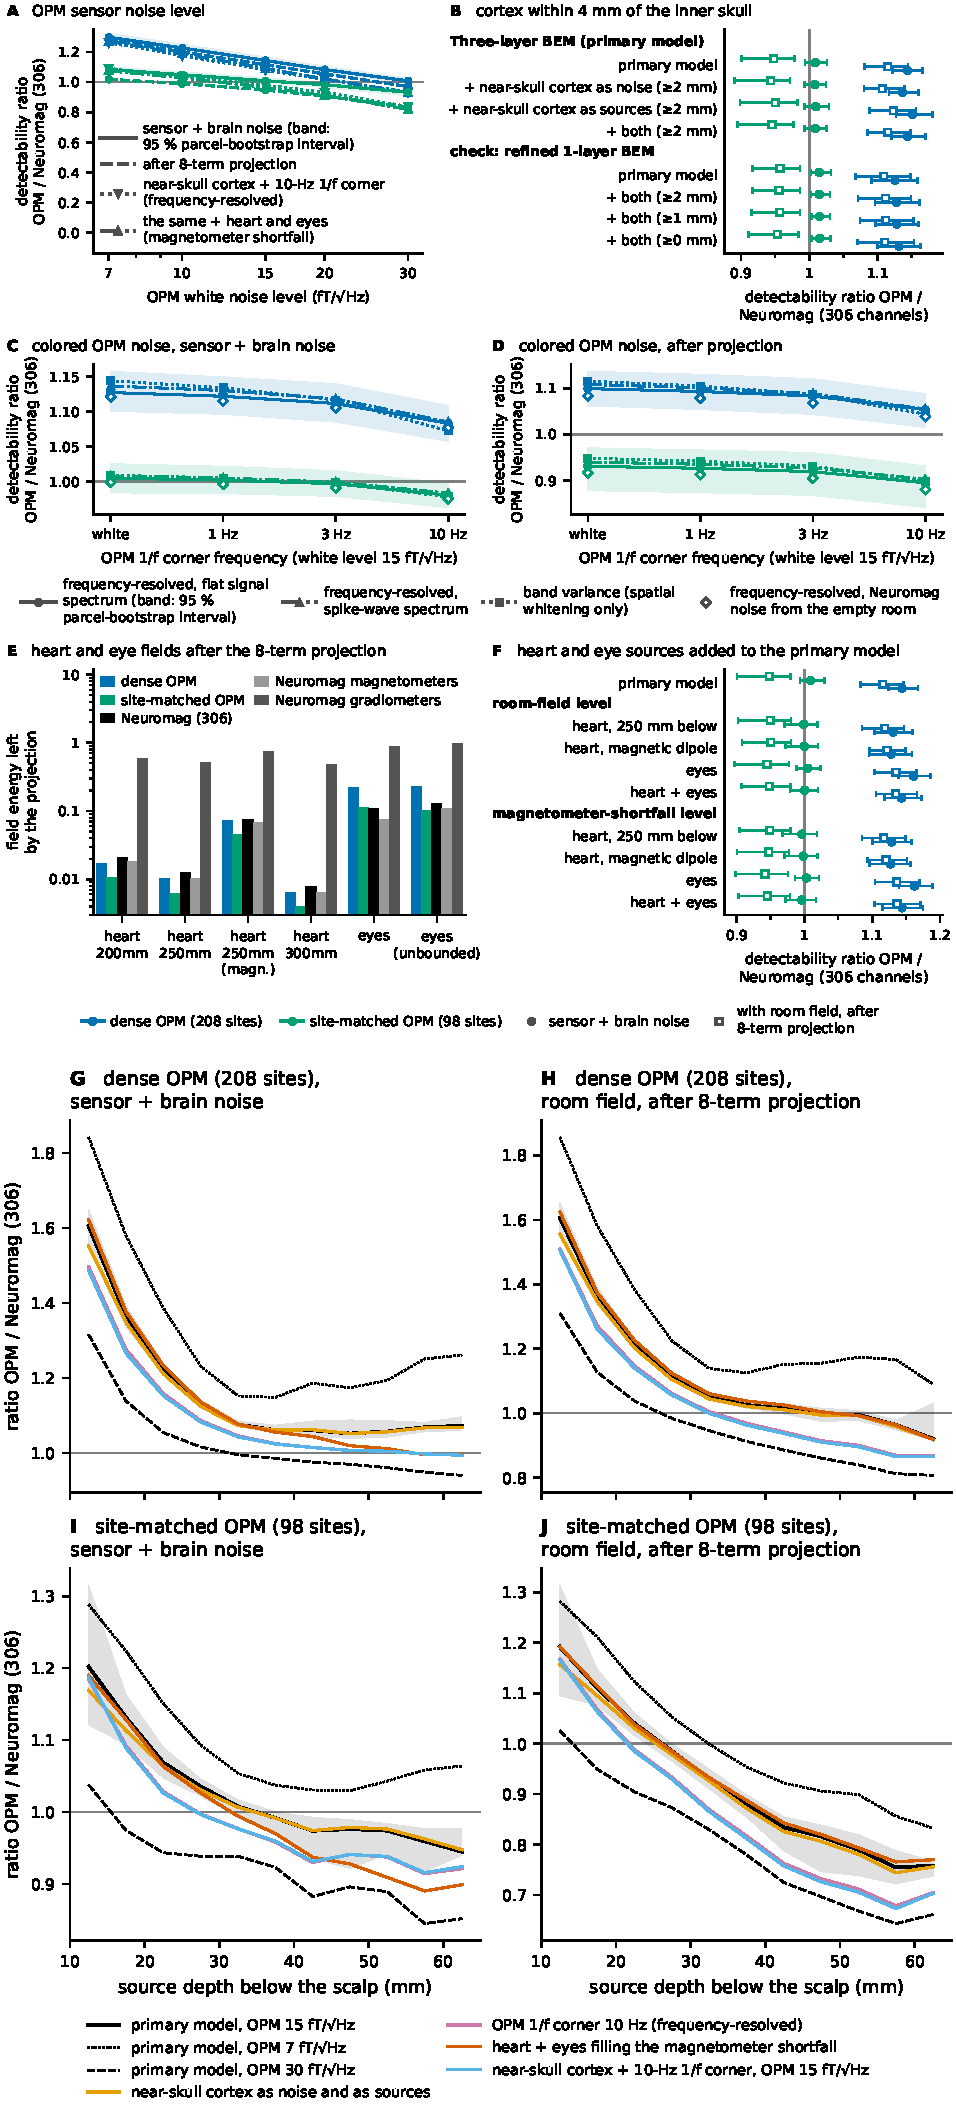
\includegraphics[width=\textwidth,height=0.78\textheight,keepaspectratio,trim=6.06bp 420.57bp 6.06bp 0.00bp,clip]{Figure_S5.pdf}
\caption{Sensitivity of the adult comparison to the noise model. Median ratio OPM/Neuromag (306 channels) over the 7,661 targets for the dense (208 sites, blue) and site-matched (98 sites, green) OPM arrays, with 95\,\% parcel-bootstrap bands or bars. In B and F, filled circles, sensor plus brain noise; open squares, room field projected out. (A) Ratio against OPM white noise (7, 10, 15, 20 and 30~fT/√Hz): primary model (solid, band); projected (dashed); near-skull cortex with a 10-Hz 1/f corner, frequency-resolved detector (dotted, inverted triangles); the same with heart and eyes at the magnetometer-shortfall level (dash-dotted, triangles). (B) Near-skull cortex as noise, sources or both (three-layer BEM), and down to the inner skull (refined single-compartment BEM). (C, D) Ratio at 15~fT/√Hz against the 1/f corner, unprojected (C) and projected (D): frequency-resolved detector with flat (circles, band) or spike-wave (triangles) signal spectrum, band-variance detector (squares, dotted), and frequency-resolved detector with Neuromag's empty-room noise (open diamonds). (E) Share of cardiac and ocular field energy left after the projection, per array and for Neuromag's magnetometers and gradiometers (logarithmic axis). (F) Ratio with these sources added at the room field's level and at the shortfall level.}
\label{fig:S5}
\end{figure}

\begin{sidewaysfigure}
\ContinuedFloat
\centering\captionsetup{font=footnotesize}
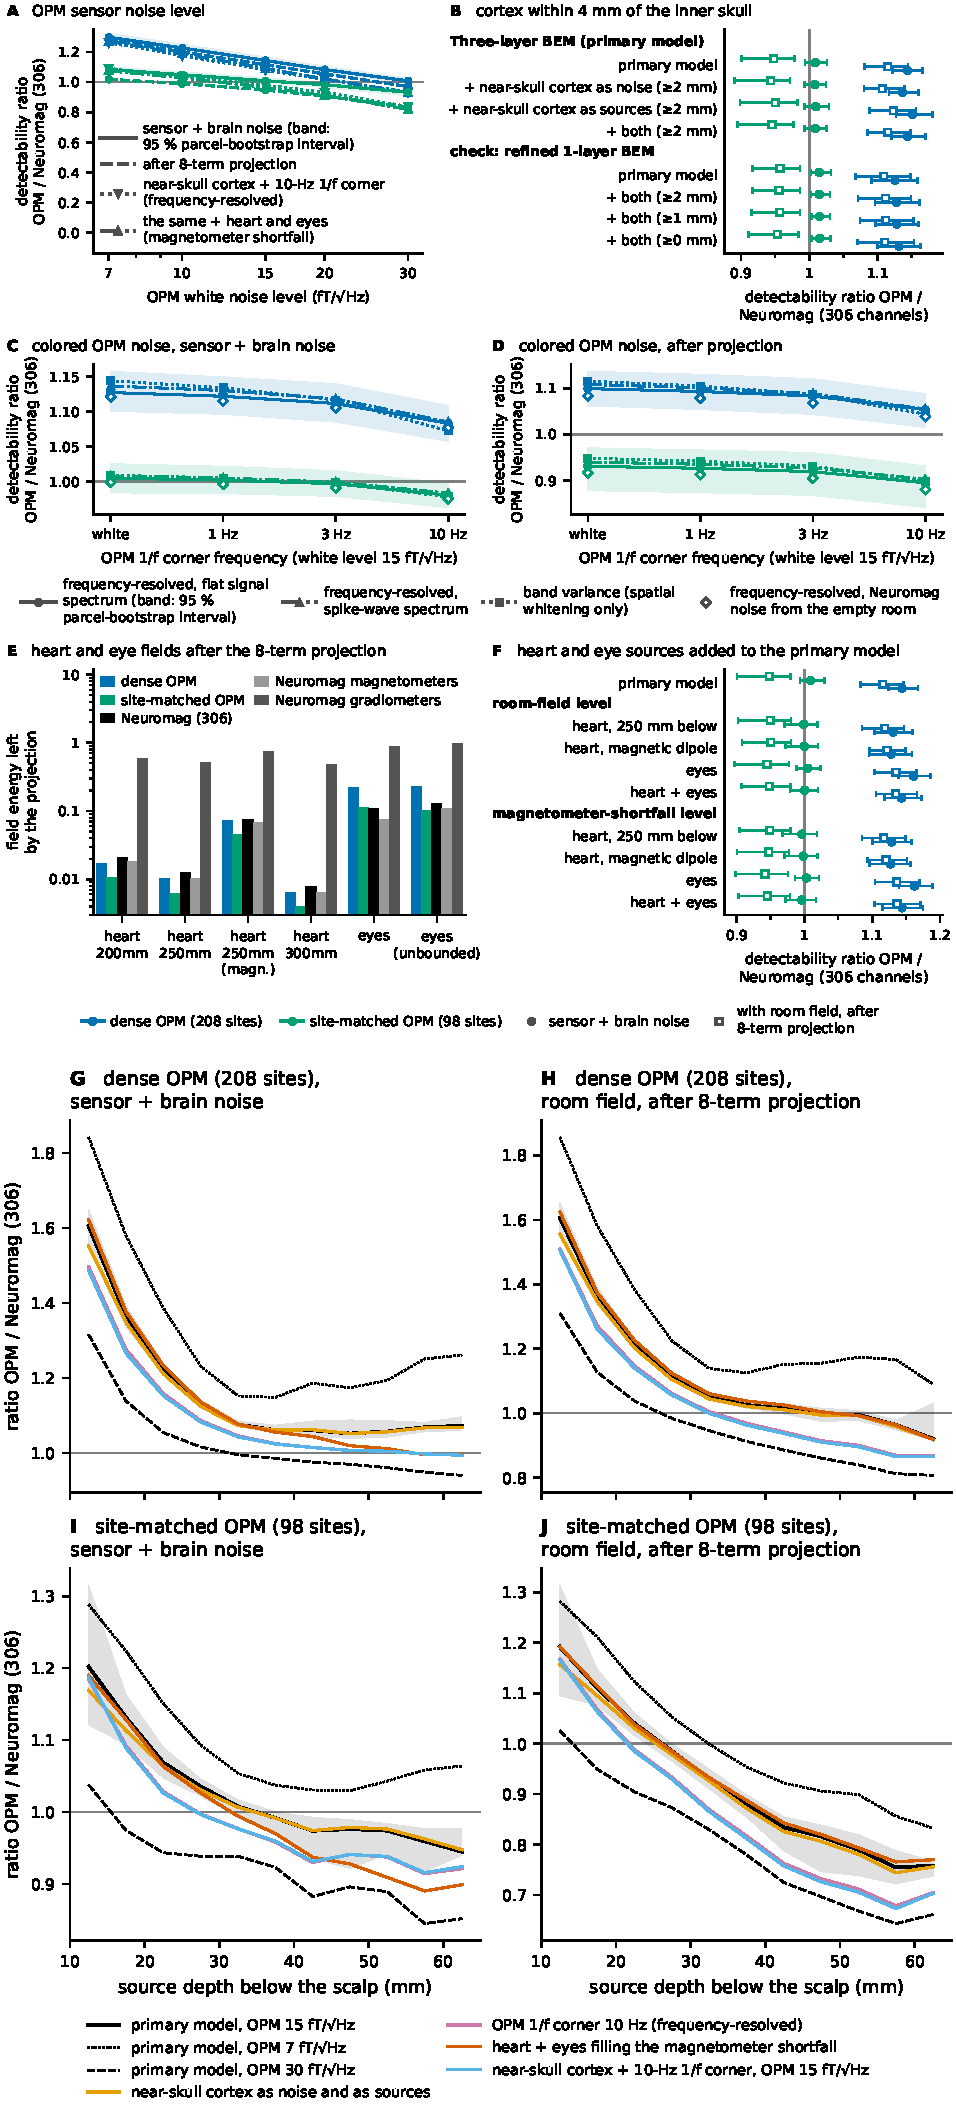
\includegraphics[width=\textheight,height=0.89\textwidth,keepaspectratio,trim=-0.00bp -0.00bp -0.00bp 728.54bp,clip]{Figure_S5.pdf}
\caption[]{(Continued.) (G--J) The ratio against depth below the scalp (5-mm bins) for the dense (G, H) and site-matched (I, J) arrays, with sensor plus brain noise (G, I) and projected (H, J). Lines: the primary model at 15~fT/√Hz (black, with band), 7~fT/√Hz (dotted) and 30~fT/√Hz (dashed); the near-skull cortex as noise and as sources; the 10-Hz corner under the frequency-resolved detector; the heart and eyes filling the magnetometer shortfall; and the near-skull cortex with the 10-Hz corner at 15~fT/√Hz.}
\end{sidewaysfigure}

\section{Head models and the MRI check}\label{sec:S4}

\subsection{The adult and the three classes of smaller head}\label{sec:S4.1}

The adult is the MNE sample subject \citep{gramfort2013}, with FreeSurfer surfaces \citep{fischl2012}, a three-layer boundary-element model (BEM) on the MRI scalp and 1,878 cm² of usable cortex. The smaller heads belong to three classes, which are not independent subjects (main text, Section 2.2). The two scaled adults keep the adult's vertices, so $\Delta$ is taken vertex by vertex: the school-age size control is 0.895 times the adult, and the 2-year size control has the head circumference of the 24-month template.

The three infant templates \citep{oreilly2021}, averages of many MRIs of the Neurodevelopmental MRI Database \citep{richards2016}, have smooth cortices. Their usable cortex at 24, 18 and 12 months, 1,062, 975 and 895 cm² (48–57\,\% of the adult's), lowers their total background power and their patch cancellation. They were used at native size with their own three-layer BEMs, oct-6 source spaces, atlas labels and fiducials.

The three school-aged children A, B and C (7.8–8.7 years; subjects sub-Z213, sub-Z209 and sub-Z226) come from the de-identified OpenNeuro dataset ds005234, released under a CC0 license \citep{fadeev2024,fadeev2025}, whose authors processed their MRIs. We used their white and sphere surfaces, atlas annotations and dense MRI scalp as distributed. In the distributed file tree, each subject's watershed BEM surfaces sit in the preceding subject's folder; we matched them to each child by the volume information they share with the child's own surfaces, and the storage objects behind them carry that child's subject name.

These surfaces put the inner skull implausibly close to the scalp (median 0.8–2.5 mm below it over the upper head), with an outer skull crossing it, so we modeled the children's skull. The inner skull was moved inward to 8 mm below the scalp wherever it lay shallower, with no vertex within 2 mm of a white-surface vertex; between vertices it comes within 0.9–1.3 mm of the white surface, and no white vertex lies outside it. The outer skull lies about halfway to the scalp, and the modeled inner skull a median 5.7–7.8 mm below the scalp over the upper head. On the adult, whose segmented skull is known, the same procedure applied to a degraded inner skull changed the primary ratio by at most 0.003 over the modeled skull depths. In every head, the forward model's outer surface is the watershed skin placed on the MRI scalp.

The dataset has no fiducials, which define the head frame and hence the centered placement, the origin of every scaled helmet and the OPM coverage region. We transferred them from the adult by a similarity fit of the cortices and moved them to the nearest scalp vertex. On the templates, this reproduced their own fiducials to within 1.6–14.4 mm (largest, 14.4 mm, at the nasion of the 18-month template, farthest from the cortex) and their head frames to within 3.2–5.9°. Such total rotations are of the order of the placement family's (pitch ±10°, yaw ±10°, roll ±5°; Section~\ref{sec:S5.1}), which indicates rather than bounds their effect; the transferred fiducials were not checked on the children's own MRIs. Fiducials from Montreal Neurological Institute (MNI) coordinates were not used: on the adult, they land 10.0–27.4 mm from the digitized ones.

Every head uses the adult's conductivities (0.3, 0.006 and 0.3 S/m). With a single-compartment BEM (0.3 S/m inside the inner skull), which needs no skull or scalp conductivity, the difference of medians from the adult was +0.19 to +1.13 dB, against +0.19 to +1.14 dB with three layers, a change of −0.06 to +0.01 dB. As distributed, the 12-month template's skull is 0.25 mm thick at its thinnest (23 of 2,562 inner-skull vertices within 1 mm of the outer skull). With the single-compartment BEM, its $D$ was +2.03 dB (three layers: +2.04 dB) and its difference from the adult +1.06 dB (+1.05 dB), so the thin skull does not carry its result.

\subsection{Regions}\label{sec:S4.2}

Regions are the lobes of the Desikan--Killiany atlas \citep{desikan2006}. Frontal: superior, rostral middle and caudal middle frontal, pars opercularis, triangularis and orbitalis, lateral and medial orbitofrontal, precentral, paracentral and frontal pole. Parietal: superior and inferior parietal, supramarginal, postcentral and precuneus. Temporal: superior, middle and inferior temporal, banks of the superior temporal sulcus, fusiform, transverse temporal, entorhinal, temporal pole and parahippocampal. Occipital: lateral occipital, lingual, cuneus and pericalcarine. Cingulate: rostral and caudal anterior, posterior and isthmus. The sixth region is the insula. The medial wall belongs to no region, and both hemispheres are pooled.

We also report parcels emphasized in the epilepsy literature, precentral, superior temporal (``lateral temporal'' in main text Fig.~7) and parahippocampal, and a group of the parahippocampal and entorhinal parcels, which is what ``mesial temporal'' always means here. With all sources on the cortical surface and no hippocampus or amygdala, this cortex (26.8–28.7 mm below the adult's scalp, median over targets) is the nearest proxy for mesial temporal generators. The regions were chosen from the literature, and rankings among them are exploratory.

\subsection{The MRI quality check of the school-aged children and the infant templates}\label{sec:S4.3}

The children's white surfaces come within 3.7–5.7 mm of the scalp used for sensor placement and source depths. Child B has 247 targets shallower than 10 mm (adult: none) and a head the size of the 24-month template's (head circumference 48.6 against 49.5 cm; cap volume 1,795 against 1,802 cm³) around a much larger cortex (1,666 against 1,062 cm²). Both suggested a scalp lying inside the true scalp or misregistered relative to the white surface. We therefore checked the children's surfaces, exactly as the forward models use them, against their T1 images, with the adult and the 24-month template as references, and then checked the 18- and 12-month templates.

The T1 intensity was sampled along the outward normal of every dense-scalp vertex, from −20 to 20 mm in 0.25-mm steps. The MRI head boundary is where this profile falls through the volume's air/tissue threshold (Otsu's method; primary), with the half-maximum edge and the steepest gradient as secondary definitions. Its signed offset from the scalp used (positive outward) was summarized over the cap, the head above the fiducial plane, by median, quartiles and 5th to 95th percentiles, and decomposed into a uniform offset, a translation and a rotation. Frames were checked by comparing each surface's volume geometry with the T1 header. White-surface registration was checked by the white/gray contrast across the surface, searching coarsely then finely for the rigid shift that maximizes it and reporting that shift's contrast gain. Head circumference and the targets below 8 and 10 mm were measured against both the boundary and the scalp used.

A head is misregistered if a surface's header differs from the T1 by more than the header tolerance, or if the white surface's realigning shift, edge translation or rotation displacement exceeds 1 mm. It is inside or outside if the cap median offset exceeds, or falls short of, the adult's by more than 1 mm (one voxel) at both the Otsu and the half-maximum edge, and usable otherwise. On the adult, a declared inward scalp displacement of 4 mm was recovered as 4.0 mm, and a 2-mm translation as 2.03 mm (97\,\% of the offset pattern explained by a translation). Undoing a 2-mm shift of its white surface raised the contrast by 65\,\%, so a misregistered white surface would be found.

Every surface's header matched its T1 (corner displacements at most 2.7 $\times 10^{-5}$ mm in the children; Fig.~\ref{fig:S6}). The children's white surfaces were registered: best realigning shift 0.0 mm, edge translation at most 0.01 mm, rotation displacement at most 0.02 mm, and contrast gains of 0\,\%, 0\,\% and 0\,\% (children A, B and C). The children's scalp used lay a median 1.3–1.5 mm inside the MRI head boundary at the Otsu edge (0.4–1.2 mm at the half-maximum edge), against 1.3 and 1.1 mm in the adult (Fig.~\ref{fig:S6}C): a FreeSurfer scalp sits just inside the T1 edge in every individual head.

The 24-month template's scalp lay 1.6 mm outside its boundary (verdict: outside), consistent with an average template whose scalp is smoothed outward; the 18- and 12-month templates' lay 1.6 and 1.3 mm outside (2.3 and 1.6 mm at the half-maximum edge, against 1.6 mm at 24 months). The verdict was outside at 12 months and misregistered at 18 months. The latter's white surface fitted the T1 contrast best after a 2.3-mm shift, gaining 41\,\% (other templates: 0.5 mm), with an edge translation of 1.7 mm, both beyond the 1-mm tolerance. This whole-surface misfit is not visible in single sections; its white vertex closest to the scalp used lies 7.3 mm below it (sections not shown). Whether it reflects a displaced surface or the weaker contrast of an average image was not settled; no template surface was repaired, and the offset was not propagated to the template's results.

The head circumference on the MRI boundary minus that on the scalp used was +8.9 to +10.7 mm in the children (49.7–54.5 against 48.6–53.5 cm) and +9.9 mm in the adult (59.6 against 58.6 cm). Measured from the boundary, the median target depth changed by +1.3 to +1.5 mm in the children, +1.3 mm in the adult and −1.7 to −1.4 mm in the templates, whose scalps lie outside their boundaries. The children's medians thus shifted as the adult's did; their shallowest targets did not.

The closest white-surface vertex lay 3.7, 3.7 and 5.7 mm below the scalp used in children A, B and C (4.6–7.5 mm below the MRI boundary), against 9.7 mm in the adult and 9.2 mm in the 24-month template (Fig.~\ref{fig:S6}A); the 5th percentiles of white-surface depth were 7.9–12.0, 14.5 and 11.8 mm. Within 8 mm of the scalp used lay 22.4, 83.4 and 3.6 cm² of the children's white surface, and within 8 mm of the MRI boundary 6.8, 28.8 and 0.1 cm² (adult: none; Fig.~\ref{fig:S6}B). In no child does the T1 head mask reach a volume face other than the inferior one, reached at the neck in children B and C as in the adult, so the field of view does not cut the head above the neck.

Of the cortical targets, 3, 18 and 0 lay below 8 mm and 43, 247 and 11 below 10 mm (adult: 0; full-precision depths). Measured to the MRI boundary, child B's targets less than 10 mm deep fell from 247 to 47. The verdicts were child A usable, child B usable and child C usable (3 of 3 usable); no surface was repaired and no analysis needed rerunning.

The children's shallow cortex, and child B's small head around a near-adult cortex, are therefore not artifacts of scalp placement or registration, judged against the adult rather than a pediatric norm. The data leave open a head boundary that the T1 images themselves place too deep, which would bring the FreeSurfer scalp, following the image's edge, toward the cortex together with the watershed surfaces (Section~\ref{sec:S4.1}); a check against the same images cannot detect it, but an independent measurement of scalp and skull over the upper head, from another sequence or modality, would. Nor can the check settle whether the white surface is anatomically correct within a few millimeters of the scalp, where the modeled scalp-and-skull layer is thinner than the adult's, or whether three children of one dataset represent their age: the verdicts test registration and scalp position, not tissue thicknesses or head circumference against norms for age.

The source rule (no source within 4 mm of the inner skull) left out 7.3\,\%, 10.0\,\% and 3.3\,\% of the white-surface area of children A, B and C, against 7.2\,\% in the adult, 9.3–10.6\,\% in the scaled adults and 0.8–2.6\,\% in the templates. The adult's share is the 7.1\,\% of Section~\ref{sec:S3.6} plus the little cortex outside the inner skull (0.05 cm² of it within 10 mm of the scalp). In the children it includes 94–100\,\% of the cortex within 8 mm of the scalp; of child B's 14,761 white-surface vertices there, 570 pass the rule. For these reasons, the main text treats the children's results as provisional geometric examples.

\begin{figure}[tbp]
\centering
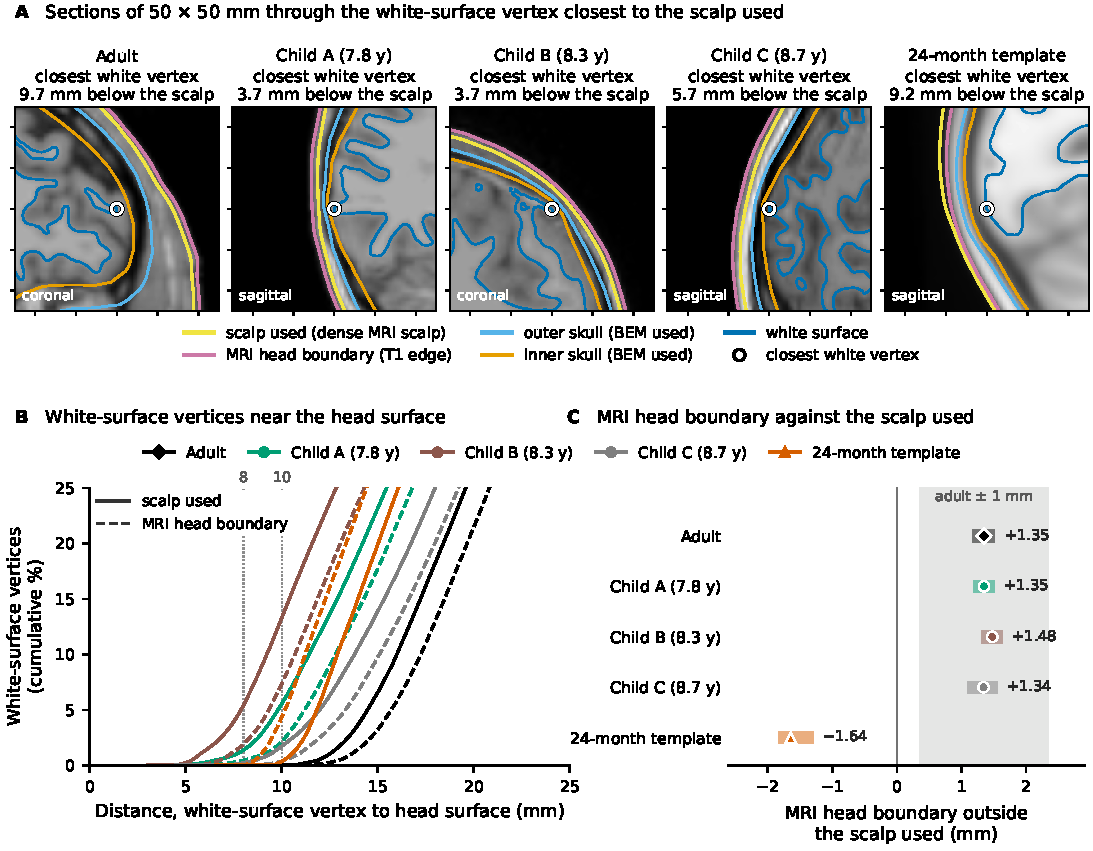
\includegraphics[width=\textwidth]{Figure_S6.pdf}
\caption{MRI quality check of the school-aged children, with the adult and the 24-month template as references; surfaces as the forward models use them. (A) Sections of 50 × 50 mm through the white-surface vertex closest to the scalp used (open circle), sagittal or coronal, whichever contains more of the scalp's outward normal there. Gray: T1 intensity; yellow: dense MRI scalp used; pink: MRI head boundary (Otsu level along the scalp normals); light blue and orange: outer and inner skull of the BEM used (modeled in the children; Section~\ref{sec:S4.1}); dark blue: white surface. (B) Cumulative share of white-surface vertices against distance to the scalp used (solid) and to the MRI head boundary (dashed), lowest quarter; dotted: the 8 and 10-mm threshold. (C) Offset of the MRI head boundary from the scalp used above the fiducial plane, positive outward: median and quartiles; shaded: the adult's median ± 1 mm, the verdict's tolerance. Children: OpenNeuro ds005234 \citep{fadeev2024,fadeev2025}; template: \citet{oreilly2021}; adult: MNE sample data. BEM, boundary-element model.}
\label{fig:S6}
\end{figure}

\section{Helmet constructions}\label{sec:S5}

\subsection{The fixed adult helmet and its placements}\label{sec:S5.1}

The centered placement puts each head's frame where the adult's lies in the sample recording (its device-to-head transform), keeping the ear line in place. The primary placement, top contact, raises the head from there until the nearest magnetometer coil center is 20 mm from the scalp, the 18-mm Dewar spacing plus a margin. This best-fit assumption, not documented practice, favors Neuromag: a child in an adult helmet may be placed centrally and repositioned toward the expected source \citep{gaetz2008}, and a small child's shoulders can stop the head short of the top \citep{tesan2010}. The other placements bound this choice.

A family of 12 source-blind placements, chosen from the geometry alone, tests the sensitivity to placement: top and back contact, shifts of ±5 mm left--right and front--back, and rotations of ±10° pitch, ±5° roll and ±10° yaw, each raised to contact (one lateral shift was infeasible for child C, leaving 11). Three further placements are the centered pose, the laterally centered pose (moved to the helmet's midline) raised to contact, and true contact at the Dewar spacing.

The adult's own $D$ was +1.27, +1.00, +1.01 and +0.87 dB at its measured pose, top contact, laterally centered contact and true contact, and it spanned +0.98 to +1.43 dB (0.46 dB) over the family, top contact ranking 2 from the lowest. Against the adult placed by the same rule, the smaller heads' $\Delta$ was +0.76 to +2.50, +0.17 to +1.07, +0.09 to +1.06 and +0.17 to +1.09 dB at the centered pose, top contact, laterally centered contact and true contact.

With sensor plus brain noise, the point estimates kept their sign against the gradiometers (+0.11 to +1.49 dB) and the magnetometers (+0.25 to +0.98 dB) and for the site-matched array (+0.08 to +1.10 dB). With the room field projected out, $\Delta$ was unchanged in the scaled adults (+0.44 to +1.09, against +0.44 to +1.07 dB), lower in the templates (+0.42 to +0.83, against +0.73 to +0.96 dB) and small in children A, B and C (+0.03 [−0.17, +0.22], +0.26 [+0.04, +0.39] and −0.19 [−0.38, +0.18] dB; child C's point estimate negative, its interval spanning zero). Their site-matched arrays gave −0.06, −0.17 and −0.10 dB, every interval including 0.

The adult's placement spread exceeded $\Delta$ in 4 of the 8 smaller heads, and each child's own $D$ varied by 0.24, 0.57 and 0.86 dB (A, B and C) over the family. Against each head's family median instead of top contact, the difference of pooled medians from the adult shrank by 0.05–0.20 dB.

The OPM arrays were refitted to each head by the adult's rules (144–174 dense and 80–91 site-matched sites on the smaller heads; median standoff 6.99–7.00 mm above each head's own MRI scalp) and kept in every helmet, with sensor noise, room field and analysis band unchanged. The background variance per unit cortical area was calibrated once on the adult, so a smaller cortex carries less total background; as a sensitivity analysis, it was multiplied by 0.5 and by 2.

Fit and head size act on $D$ through at least four routes: a wider SQUID gap and a shallower cortex raise it, whereas fewer OPM sites and, in the school-aged children, a near-adult cortex close to the OPMs (unverified near-scalp anatomy; Section~\ref{sec:S4.3}) lower it. The constructions below combine these routes differently, and none isolates one (main text, Section 3.5).

\subsection{The helmet scaled with the head}\label{sec:S5.2}

Every coil center is scaled about the head origin by the child-to-adult ratio of head circumferences, keeping coil size, orientation and noise, and the factor is raised in steps until no coil is within 18 mm of the scalp; unlike the sphere's constant gap (Section~\ref{sec:S2}), the gaps scale with the head. The helmet was scaled about the centered head and, as a variant added after the first pediatric results were known to remove the templates' lateral offset, about the laterally centered head. The construction asks what the adult's fit would give at a child's size and is not a pediatric SQUID device; the main text treats it as secondary because it also brings the sensors closer than the adult's own fit (see below).

Scaled about the laterally centered head, $\Delta$ against the adult in its own scaled helmet was −0.76 to +0.04 dB, the highest upper interval bound, child C's, being +0.20 dB (parcel-bootstrap intervals exclude placement and construction uncertainty). Only child C, whose helmet keeps a median gap of 33.1 mm against the adult's 29.6 mm, was not negative (+0.04 [−0.20, +0.20] dB, an interval that also contains its fixed-helmet $\Delta$). With the room field projected out, the difference of medians from the adult was −0.92 to −0.10 dB (−0.67 to +0.05 dB with sensor plus brain noise).

Scaled about the centered head, the helmet left residual gains in the off-center heads, the 24- and 18-month templates and child C (+0.24, +0.18 and +0.56 dB; $\Delta$ −0.74 to +0.56 dB overall). The OPM kept its absolute advantage in the scaled helmet ($D$ +0.62 to +1.33 dB in the smaller heads), but the additional child--adult contrast is no longer established.

Three checks qualify this result. First, part of the drop comes from the reference: against the adult at top contact, the difference of medians was −0.38 to +0.33 dB (child C +0.33 dB, above its fixed-helmet $\Delta$). Second, the gap scales with the helmet and shrank below the adult's 29.6 mm in 7 of the 8 smaller heads (25.1–28.0 mm), a tighter fit than the adult's that favors Neuromag and that the helmet fitted at the adult's gap avoids (Section~\ref{sec:S5.3}). Third, the smaller heads carry fewer OPM sites (144–174 against 208); the adult's array subsampled to those counts lost 0.27–0.53 dB, so at an equal OPM site count $\Delta$ in the fixed helmet would be +0.43 to +1.43 dB.

\subsection{The helmet fitted at the adult's gap}\label{sec:S5.3}

The Neuromag helmet is scaled about the head origin of each head's laterally centered pose until the median gap from magnetometer coil center to scalp equals the adult's: 29.6 mm, the adult's gap in its own helmet about its laterally centered head (scale factor 1.000), or, as a variant, 28.4 mm, its gap at top contact in the fixed helmet. Coil size, orientation, integration points and noise are kept, and no coil center may come within the 18-mm Dewar spacing of the scalp or lie inside the head. In child C, this clearance binds first: the helmet stops at a gap of 32.8 mm, 3.3 mm above the target, with a scale factor of 0.941 instead of 0.920.

Because the OPM arrays are those of the fixed helmet, the within-head contrast (the median over a head's targets of the target-wise difference between $D$ at top contact in the fixed helmet and $D$ in the fitted helmet) is a property of Neuromag alone, whichever OPM array is compared. Intervals use 1,000 parcel-bootstrap resamples for the dense array in the fixed helmet and in the helmet fitted at 29.6 mm, and 200 elsewhere. The fitted helmet (Table~\ref{tab:S5}) is a geometric control at the adult's median gap, not at its gap distribution, placement or coverage, and not a pediatric SQUID system.

\begin{table}[tbp]
\caption{The helmets per head. Median gap from magnetometer coil center to scalp in the fixed adult helmet at top contact, in the helmet scaled with the head about the laterally centered head, and in the helmet fitted at the adult's gap (29.6 mm) with its scale factor $k$; and $k$ for the variant fitted at the adult's top-contact gap (28.4 mm).}
\label{tab:S5}
\centering
\footnotesize
\begin{tabularx}{\textwidth}{L{2.7cm}YYYYY}
\toprule
Head & Gap, fixed helmet (mm) & Gap, scaled with the head (mm) & Gap, fitted at the adult's gap (mm) & $k$, fitted & $k$, fitted at the top-contact gap \\
\midrule
Adult & 28.4 & 29.6 & 29.6 & 1.000 & 0.991 \\
School-age size & 34.1 & 26.6 & 29.6 & 0.916 & 0.908 \\
2-year size & 39.1 & 25.1 & 29.6 & 0.876 & 0.868 \\
24-month template & 38.5 & 27.0 & 29.6 & 0.881 & 0.873 \\
18-month template & 38.9 & 27.2 & 29.6 & 0.880 & 0.872 \\
12-month template & 40.4 & 27.7 & 29.6 & 0.855 & 0.846 \\
Child A & 35.2 & 26.1 & 29.6 & 0.921 & 0.913 \\
Child B & 38.4 & 28.0 & 29.6 & 0.877 & 0.867 \\
Child C & 32.6 & 33.1 & 32.8$^{a}$ & 0.941 & 0.941 \\
\bottomrule
\end{tabularx}
\tablenotes{$^{a}$ Clearance-bound: the helmet stops at the 18-mm Dewar spacing before the target gap is reached. Gap: median over the magnetometer coil centers of the distance to the nearest scalp point; $k$: scale factor of the helmet about the head origin.}
\end{table}

At the adult's gap (Table~\ref{tab:S6}), $\Delta$ was +0.02 to +0.03 dB in the scaled adults, +0.04 to +0.15 dB in the templates and −0.39 to +0.01 dB in the children. Its intervals included zero in 5 heads, lay below zero in 2 and above zero in 1. The site-matched array, the projected condition and the variant at the top-contact gap gave −0.45 to +0.13, −0.67 to −0.05 and −0.36 to +0.13 dB.

Against the adult at top contact in the fixed helmet, the heads fitted at the adult's top-contact gap differed from it by +0.10 to +0.23 dB in the scaled adults and templates (4 of 5 intervals above zero) and by −0.11 [−0.40, +0.06], −0.22 [−0.35, +0.01] and +0.30 [−0.02, +0.61] dB in children A, B and C. This residual depends on the adult's placement. The interaction, which places the adult by the same rule in both helmets, was +0.40 to +1.11 dB in the scaled adults and templates at the top-contact gap. In the fitted helmet, the dense array kept its absolute advantage in every head ($D$ +0.97 to +1.32 dB), and the site-matched array's $D$ was −0.09 to +0.33 dB with sensor plus brain noise and −0.96 to −0.10 dB projected.

\begin{landscape}
\begin{table}[p]
\caption{The helmet fitted at the adult's gap, per head. Dense OPM array against Neuromag (306 channels) with sensor plus brain noise unless stated; values in dB; brackets: 95\,\% parcel-bootstrap intervals within the head.}
\label{tab:S6}
\centering
\footnotesize
\begin{tabularx}{\linewidth}{L{2.3cm}YL{1.6cm}L{1.6cm}L{1.9cm}YYY}
\toprule
Head & $\Delta$, dense (dB) & $\Delta$, site-matched (dB) & $\Delta$, dense, projected (dB) & $\Delta$, dense, at the top-contact gap (dB) & Within-head contrast (dB) & Interaction (non-additivity) (dB) & $\Delta$ at equal OPM site count (dB) \\
\midrule
School-age size & +0.03\newline [0.00, +0.05] & +0.03 & −0.05 & +0.02 & +0.17\newline [+0.08, +0.28] & +0.40\newline [+0.30, +0.50]\newline (+0.02) & +0.20\newline [+0.16, +0.24] \\
2-year size & +0.02\newline [−0.02, +0.06] & +0.12 & −0.07 & +0.01 & +0.76\newline [+0.64, +0.90] & +1.10\newline [+0.97, +1.21]\newline (−0.05) & +0.30\newline [+0.24, +0.35] \\
24-month template & +0.04\newline [−0.06, +0.19] & +0.02 & −0.25 & +0.02 & +0.34\newline [+0.20, +0.54] & +0.54\newline [+0.44, +0.73]\newline (+0.15) & +0.42\newline [+0.29, +0.68] \\
18-month template & +0.15\newline [−0.08, +0.33] & −0.02 & −0.21 & +0.13 & +0.42\newline [+0.27, +0.61] & +0.70\newline [+0.45, +0.83]\newline (+0.03) & +0.42\newline [+0.22, +0.69] \\
12-month template & +0.05\newline [−0.09, +0.24] & −0.07 & −0.25 & +0.02 & +0.55\newline [+0.38, +0.78] & +0.66\newline [+0.56, +0.99]\newline (+0.24) & +0.49\newline [+0.33, +0.81] \\
Child A & −0.30\newline [−0.48, −0.22] & −0.26 & −0.67 & −0.27 & +0.29\newline [+0.19, +0.40] & +0.53\newline [+0.44, +0.70]\newline (+0.08) & +0.16\newline [−0.12, +0.23] \\
Child B & −0.39\newline [−0.54, −0.17] & −0.45 & −0.50 & −0.36 & +0.42\newline [+0.27, +0.61] & +0.71\newline [+0.58, +0.77]\newline (+0.09) & +0.16\newline [−0.10, +0.41] \\
Child C & +0.01\newline [−0.23, +0.18] & +0.13 & −0.27 & +0.11 & −0.12\newline [−0.20, −0.02] & +0.04\newline [−0.11, +0.19]\newline (+0.13) & +0.48\newline [+0.14, +0.62] \\
\bottomrule
\end{tabularx}
\tablenotes{$\Delta$: against the adult in its own fitted helmet ($D$ = +1.28 dB). Projected: room field projected out. Within-head contrast and interaction: Section~\ref{sec:S5.3} (adult's contrast, −0.23 dB); the interaction is taken like $\Delta$, per vertex for the scaled adults and per parcel for the templates and children, so it is not the difference of the medians in the previous column. In parentheses, the non-additivity $\Delta$(fixed) − $\Delta$(fitted) − interaction of the area-weighted medians. In the school-age size head, the lower bound of the dense $\Delta$ rounds to 0.00 from above. $\Delta$ at equal OPM site count: with the adult's dense array subsampled to the head's dense site count. OPM, optically pumped magnetometer.}
\end{table}
\end{landscape}

The within-head contrast, what Neuromag loses in a head to the fit, gap and placement of the fixed helmet together, was +0.17 to +0.76 dB in the scaled adults, +0.34 to +0.55 dB in the templates and −0.12 to +0.42 dB in the children. The adult's was −0.23 dB, because its laterally centered pose in its own helmet is looser than top contact. Child C's was negative although its fixed-helmet gap (32.6 mm) and clearance-bound fitted gap (32.8 mm) nearly coincide; at an equal median gap, the fitted construction itself is worth −0.11 [−0.15, −0.08] dB in the adult, so this contrast is one of construction, not of gap.

The interaction, a smaller head's contrast minus the adult's, is the extra that the fixed helmet gives a smaller head beyond the adult: +0.40 to +1.10 dB in the scaled adults, +0.54 to +0.70 dB in the templates and +0.04 to +0.71 dB in the children. At every vertex of a scaled adult it equals $\Delta$(fixed) − $\Delta$(fitted), but the area-weighted medians of these quantities are not additive (residual in Table~\ref{tab:S6}), so the within-head and interaction estimates are reported in their own right.

For equal OPM site counts, the adult's dense array was subsampled by farthest-point sampling to each smaller head's dense site count (144–174 sites), the adult in the same fitted helmet. At the adult's gap, $\Delta$ was then +0.16 to +0.49 dB: +0.20 to +0.30 dB in the scaled adults, +0.42 to +0.49 dB in the templates and +0.16 to +0.48 dB in the children (the intervals of children A and B include zero). A smaller head's dense array thus gains a little at the adult's median gap and equal site count, possibly, though these controls do not test it, because its cortex lies closer to the OPMs. The fewer sites take about that much back in the scaled adults and templates and more in children A and B, where what else lowers $\Delta$ is not settled by these controls (provisional examples; Sections~\ref{sec:S4.3} and \ref{sec:S5.5}).

As a measure of placement uncertainty, $\Delta$ in the fixed helmet was computed at each of the 12 source-blind placements (Table~\ref{tab:S7}). $\Delta$ was positive at every placement in every head except child C. The crossed band is wider and includes zero in the children. Top contact was not an extreme of any band.

\begin{table}[tbp]
\caption{Placement bands of $\Delta$ in the fixed adult helmet. Dense OPM array against Neuromag (306 channels), sensor plus brain noise.}
\label{tab:S7}
\centering
\footnotesize
\begin{tabularx}{\textwidth}{L{2.6cm}cYcYYY}
\toprule
Head & $n$ & Band (dB) & Span (dB) & Rank of top contact & Crossed band (dB) & $\Delta$ at top contact (dB) \\
\midrule
School-age size & 12 & +0.20 to +1.12 & 0.92 & 9 & +0.03 to +1.58 & +0.44\newline [+0.34, +0.56] \\
2-year size & 12 & +0.67 to +1.61 & 0.94 & 8 & +0.26 to +2.07 & +1.07\newline [+0.91, +1.18] \\
24-month template & 12 & +0.48 to +1.38 & 0.90 & 7 & +0.32 to +1.53 & +0.73\newline [+0.46, +0.98] \\
18-month template & 12 & +0.54 to +1.36 & 0.82 & 11 & +0.37 to +1.51 & +0.88\newline [+0.54, +1.05] \\
12-month template & 12 & +0.75 to +1.66 & 0.92 & 10 & +0.55 to +1.82 & +0.96\newline [+0.61, +1.51] \\
Child A & 12 & +0.06 to +0.37 & 0.30 & 10 & −0.18 to +0.52 & +0.30\newline [+0.11, +0.38] \\
Child B & 12 & +0.19 to +0.63 & 0.44 & 9 & −0.03 to +0.99 & +0.41\newline [+0.28, +0.54] \\
Child C & 11 & −0.10 to +0.70 & 0.80 & 5 & −0.38 to +0.94 & +0.17\newline [−0.07, +0.34] \\
\bottomrule
\end{tabularx}
\tablenotes{Band: $\Delta$ at each source-blind placement, each head against the adult at the same placement, as a difference of area-weighted medians; $n$: feasible placements; rank: of top contact from the lowest $\Delta$ of the band; crossed band: any feasible placement of the head against any placement of the adult. Last column: the primary $\Delta$ at top contact with its 95\,\% parcel-bootstrap interval. OPM, optically pumped magnetometer.}
\end{table}

\subsection{Depth matching}\label{sec:S5.4}

Depth is the route of head size that the sphere describes (Section~\ref{sec:S2}). The templates' and children's cortex is shallower than the adult's: area-weighted median depths were 20.6–23.2 and 20.0–23.4 mm, against 26.2 mm, and 36–46\,\% and 35–47\,\% of the cortical area lay 10–20 mm below the scalp, against 21\,\% in the adult. Reweighting each head's targets to the adult's depth distribution lowered the difference of pooled medians from the adult in the fixed helmet, from +0.85 to +1.05 to +0.29 to +0.53 dB in the templates and from +0.19 to +0.52 to −0.05 to +0.05 dB in the children.

Within depth strata, $\Delta$ (the difference of the two heads' area-weighted medians) was positive in every stratum of the scaled adults and templates (+0.11 to +1.62 dB; Fig.~\ref{fig:S7}A). For the children, it was negative in 11 of the 12 child-strata at 10–30 mm (−0.36 to +0.08 dB), with no interval above zero (largest lower bound −0.25 dB), and positive deeper (+0.01 to +1.77 dB; Fig.~\ref{fig:S7}B). In this decomposition, their shallower cortex matches their fixed-helmet gain. The depths are measured from the scalp used, unverified near the scalp in the children; measured from the MRI boundary, the children's median depths shift as the adult's do (Section~\ref{sec:S4.3}). The decomposition describes the model's surfaces, not a tested mechanism.

In the helmet fitted at the adult's gap, the children's strata were negative throughout the depths that hold most of their cortex: for child A, $\Delta$ was −1.70, −0.91 and −0.20 dB at 10–15, 20–25 and 30–40 mm, its intervals including zero only from the 40–50 mm stratum down. The two decompositions, fitting the helmet and matching depth, are not additive, and neither apportions the routes exactly.

\begin{figure}[tbp]
\centering
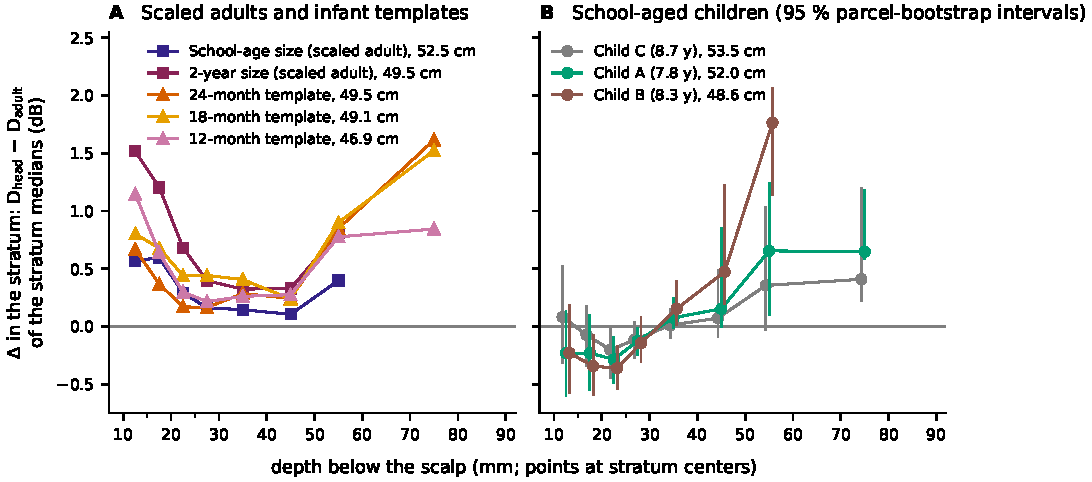
\includegraphics[width=\textwidth]{Figure_S7.pdf}
\caption{$\Delta$ within depth strata in the fixed adult helmet. Difference of the two heads' area-weighted medians within strata of depth below each head's own scalp (points at stratum centers); top contact, dense OPM array against Neuromag (306 channels), sensor plus brain noise. (A) Scaled adults and infant templates. (B) School-aged children, with 95\,\% intervals from parcels resampled in each anatomy independently (1,000 resamples). Strata with fewer than 10 targets in either head are omitted. OPM, optically pumped magnetometer.}
\label{fig:S7}
\end{figure}

\subsection{Noise in the smaller heads and the share of cortex where the OPM is ahead}\label{sec:S5.5}

With the adult's background variance per unit cortical area in every head, the noise differs between classes of head. In the fixed helmet, Neuromag's magnetometer brain noise fell from 202 fT in the adult at top contact (192 fT at its measured pose) to 98–150 fT in the templates and scaled adults. Their wider gap and smaller cortex both contribute, and the shares were not separated: moving the school-age size control from its centered pose to top contact raised this noise from 131 to 150 fT. A smaller cortex does not lower the field at sensors that stay close, as the OPMs show (525 and 537 fT in the scaled adults, against 494 fT in the adult).

The children's cortex is nearly adult-sized (1,666–1,869 cm²), so Neuromag's brain noise stayed at 168–194 fT, and the OPMs, close to a near-adult cortex that lies near the scalp in these surfaces (unverified there; Section~\ref{sec:S4.3}), saw more of it (617–751 fT).

The share of cortex on which the OPM is ahead, the kind of metric used by \citet{jas2026}, is saturated for the dense array (99.6\,\% of cortical area in the adult). For the site-matched array it was 49\,\% in the adult at top contact (56\,\% of all targets at the measured pose) and 58–89\,\% in the smaller heads in the fixed helmet (Fig.~\ref{fig:S8}C).

\begin{figure}[tbp]
\centering
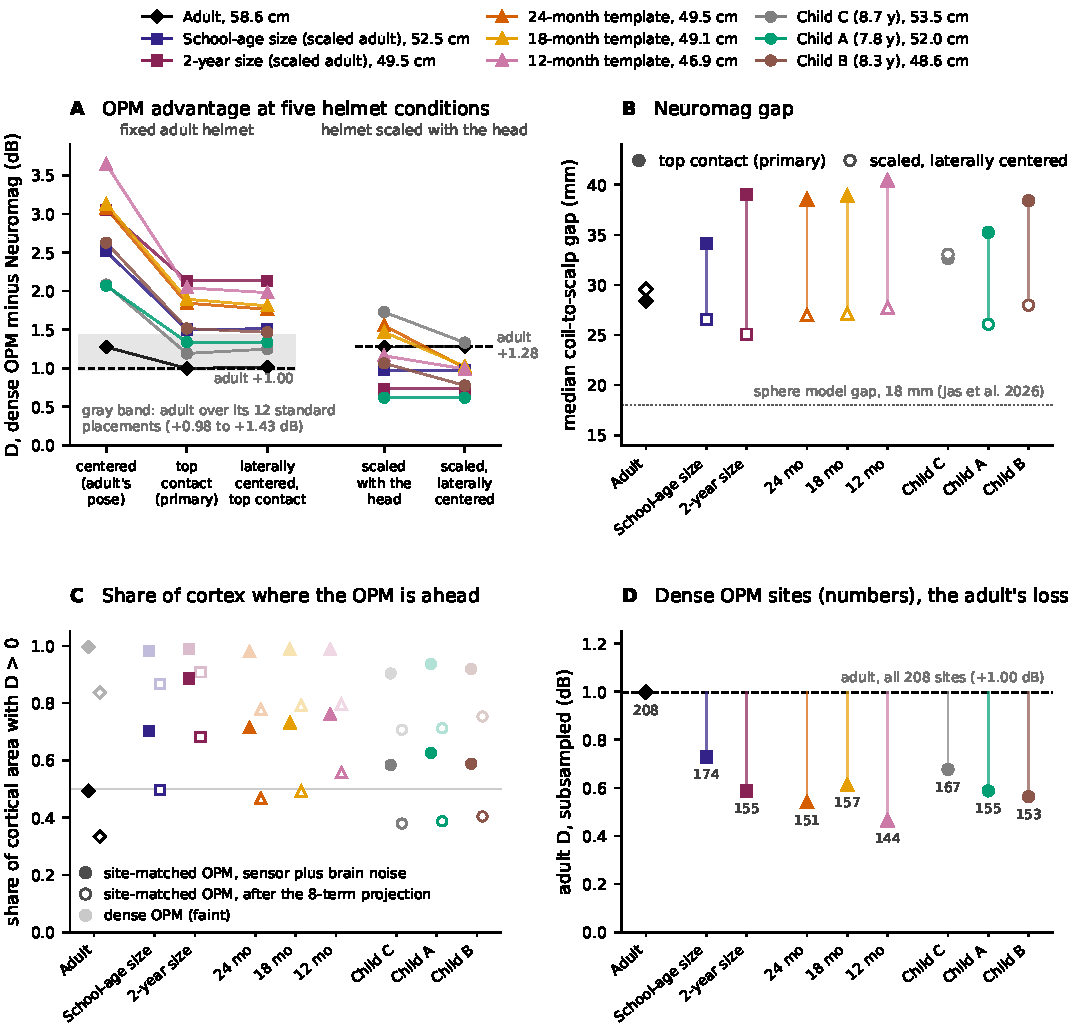
\includegraphics[width=\textwidth]{Figure_S8.pdf}
\caption{The helmet scaled with the head and the routes of head size. Dense OPM array against Neuromag (306 channels), sensor plus brain noise; $D$, area-weighted median over cortical targets; heads ordered by class and head circumference. (A) $D$ under five helmet conditions: the fixed adult helmet at the centered pose, at top contact (primary) and laterally centered at top contact, and the helmet scaled with the head about the centered and the laterally centered head. Dashed lines: the adult at top contact and in its own scaled, laterally centered helmet (+1.28 dB); gray band: the adult over its 12 source-blind placements. (B) Median gap from magnetometer coil to scalp at top contact (filled) and in the scaled, laterally centered helmet (open); dotted: the 18-mm gap of the spherical benchmark \citep{jas2026}. (C) Share of cortical area with $D > 0$ at top contact, site-matched array (filled: sensor plus brain noise; open: room field projected out) and dense array (faint). (D) Dense OPM sites per head (numbers) and the adult's $D$ with its array subsampled to each count. The helmet fitted at the adult's gap is shown in main text Fig.~9. OPM, optically pumped magnetometer.}
\label{fig:S8}
\end{figure}

\section{Regions and the noise floor across heads}\label{sec:S6}

Unless stated otherwise, $D$ is the dense optically pumped magnetometer (OPM) array's detectability relative to Neuromag's 306 channels in dB (Section~\ref{sec:S1}), the area-weighted median over the cortical targets of a head or region (both hemispheres), with sensor plus brain noise. The helmets are those of Section~\ref{sec:S5}.

\subsection{Regions by head}\label{sec:S6.1}

In the fixed adult helmet at top contact, the dense array was ahead in every region of every head ($D$ +0.25 to +3.06 dB over the cells of Fig.~\ref{fig:S9}A), and a smaller head exceeded the adult's value for the same region in 72 of 80 cells. Of the six lobes, the temporal lobe gained most in the infant templates (+2.63, +2.88 and +3.02 dB at 24, 18 and 12 months, against +1.17 dB in the adult).

The parahippocampal and mesial temporal rows, the adult's lowest temporal rows (+0.74 and +0.74 dB), were higher in every template and scaled adult. The mesial temporal group reached +1.16 to +2.79 dB in the templates and scaled adults but +0.46 to +1.77 dB in the children, child C (+0.46 dB) lying below the adult. The cingulate was the lowest row in every head (+0.25 dB in the adult, +0.26 to +0.61 dB in the smaller heads).

The peak-channel signal-to-noise ratio (SNR; sensor plus brain noise) gave a different picture. Against the magnetometers alone, the dense array was ahead in every head (+1.84 dB in the adult at top contact, +2.05 to +2.71 dB in the smaller heads). Against Neuromag's best channel, Neuromag led in the adult (−1.11 dB) and in 4 of the 8 smaller heads (−0.85 to +0.79 dB), the children among them (−0.64, −0.28 and −0.85 dB in A, B and C).

In the helmet scaled with the head (lobes only; Fig.~\ref{fig:S9}B), the regional gain was smaller, by how much depending on the reference: 39 of the 48 lobe cells of the smaller heads were at or below the adult's in its own scaled helmet, and 28 at or below the adult's at top contact (17 of 30 for the templates and scaled adults, 11 of 18 for the children), counting point estimates without a tolerance. The children's lobes ranged from +0.17 to +1.62 dB in the scaled helmet.

In the helmet fitted at the adult's gap (Table~\ref{tab:S8}), the scaled adults kept the adult's ordering (frontal, precentral and superior temporal cortex highest; cingulate and insula lowest), and the cingulate was the lowest row in every head except the children, where the insula lay just below it. The templates and children reordered the upper rows: parahippocampal and mesial temporal rows were high in the 24- and 18-month templates and in child B, and the occipital lobe was highest in child C.

The children differed from the adult by region in both directions. Child B was below the adult in the frontal lobe (−0.81 dB) and the precentral gyrus (−0.63 dB) but above it in the parahippocampal (+0.86 dB) and occipital (+0.23 dB) cortex, and child C was below it in the entorhinal cortex (−1.02 dB) but above it in the occipital lobe (+0.64 dB).

The cortical maps (Fig.~\ref{fig:S10}; main text, Fig. 8C) show $D$ largest on the lateral convexity, most on gyral crowns, with medial surfaces near zero. By region, then, the ordering changed with the helmet; the relative weight of helmet and region was not quantified. Heat maps and cortical maps show point estimates, and the pediatric intervals represent within-anatomy resampling only.

\begin{table}[tbp]
\caption{Regional $D$ in the helmet fitted at the adult's gap. Dense OPM array against Neuromag (306 channels), sensor plus brain noise; area-weighted median over the region's targets, both hemispheres; point estimates.}\label{tab:S8}
\centering\footnotesize\setlength{\tabcolsep}{3pt}
\begin{tabular}{lrrrrrrrrr}
\toprule
 & \multicolumn{9}{c}{$D$ (dB)} \\
\cmidrule(l){2-10}
Region & Adult & School & 2-y & 24 mo & 18 mo & 12 mo & Child A & Child B & Child C \\
\midrule
Frontal & +1.82 & +1.80 & +1.77 & +1.89 & +2.05 & +2.19 & +1.22 & +1.01 & +1.52 \\
Parietal & +1.15 & +1.34 & +1.22 & +1.05 & +0.97 & +1.02 & +0.74 & +0.89 & +1.53 \\
Temporal & +1.32 & +1.28 & +1.20 & +1.40 & +1.50 & +1.35 & +1.13 & +1.21 & +1.03 \\
Occipital & +0.95 & +0.93 & +0.85 & +0.82 & +0.79 & +0.74 & +1.18 & +1.18 & +1.58 \\
Cingulate & +0.40 & +0.41 & +0.39 & +0.56 & +0.50 & +0.46 & +0.30 & +0.37 & +0.41 \\
Insula & +0.71 & +0.66 & +0.67 & +1.08 & +0.96 & +0.74 & +0.28 & +0.32 & +0.40 \\
Precentral & +1.79 & +1.70 & +1.57 & +1.56 & +1.73 & +1.91 & +1.10 & +1.16 & +1.56 \\
Superior temporal & +1.39 & +1.50 & +1.22 & +1.09 & +1.27 & +1.11 & +0.96 & +0.71 & +0.94 \\
Parahippocampal & +0.88 & +0.87 & +1.01 & +1.97 & +2.25 & +0.88 & +0.81 & +1.74 & +1.49 \\
Mesial temporal & +0.91 & +0.82 & +0.93 & +1.80 & +2.01 & +1.10 & +0.37 & +1.32 & +0.76 \\
\bottomrule
\end{tabular}
\tablenotes{Mesial temporal: parahippocampal and entorhinal cortex together. School and 2-y: the school-age and 2-year size controls (scaled adults); 24, 18 and 12 mo: the infant templates; Child A--C: the school-aged children. $D$: OPM detectability relative to Neuromag; OPM: optically pumped magnetometer.}
\end{table}

\begin{figure}[tbp]
\centering
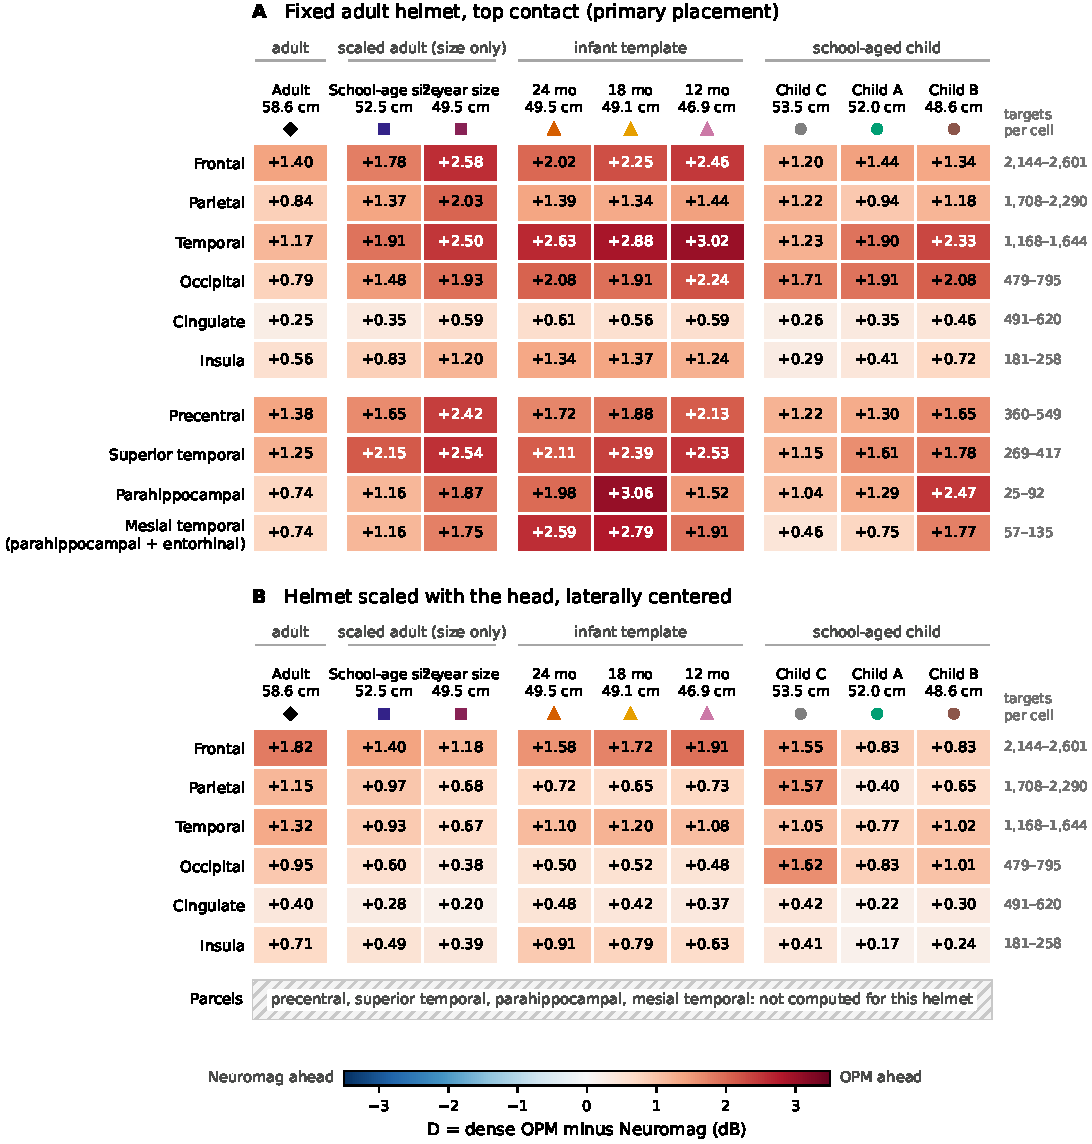
\includegraphics[width=\textwidth]{Figure_S9.pdf}
\caption{Brain regions that favor the OPM at each head size. Area-weighted median $D$ (dense OPM array against Neuromag, 306 channels; sensor plus brain noise) by lobe and for the precentral, superior temporal, parahippocampal and mesial temporal (parahippocampal and entorhinal) cortex; both hemispheres, medial wall excluded; numbers at right, targets per row (range over heads). Heads are grouped by class and ordered by head circumference (46.9–58.6 cm). (A) Fixed adult helmet at top contact. (B) Helmet scaled with the head, laterally centered; parcel rows hatched, not computed for this helmet (Table~\ref{tab:S8} gives them for the fitted helmet). Shared color scale centered at 0 dB; point estimates. $D$, OPM detectability relative to Neuromag.}\label{fig:S9}
\end{figure}

\begin{figure}[tbp]
\centering
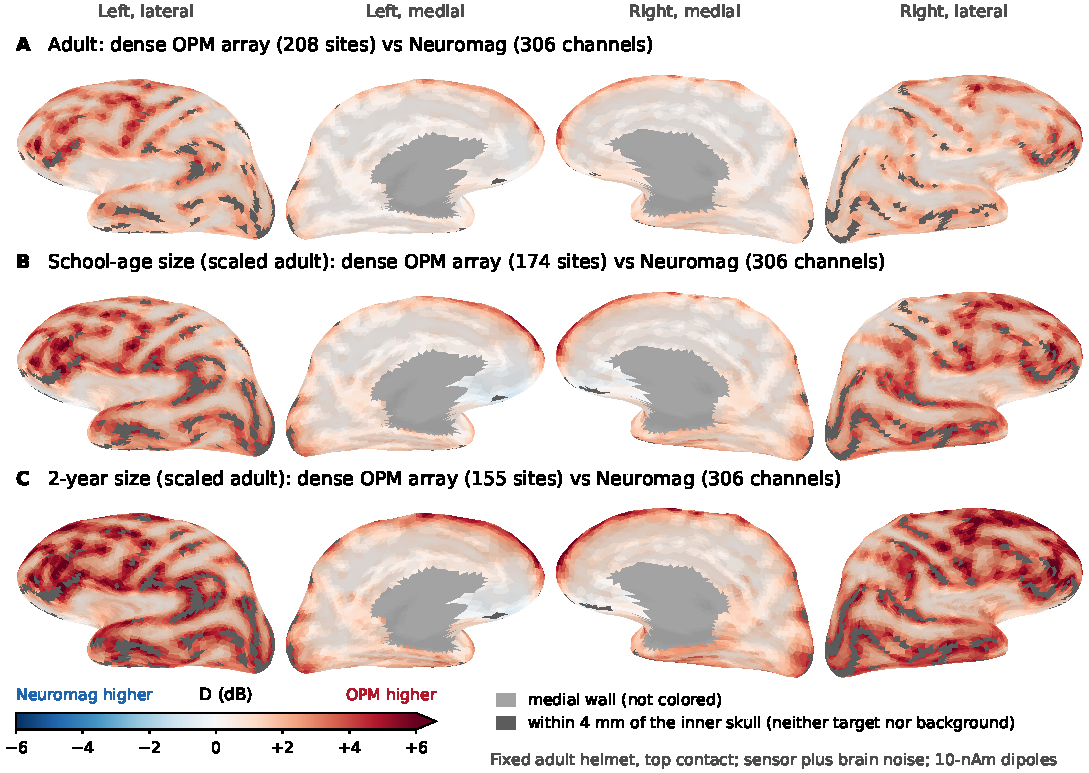
\includegraphics[width=\textwidth]{Figure_S10.pdf}
\caption{Cortical maps of $D$ in the adult and the scaled adults. Dense OPM array against Neuromag (306 channels), fixed adult helmet at top contact, sensor plus brain noise; inflated cortex, lateral and medial views of both hemispheres. (A) Adult (208 dense sites; area-weighted median $D$ +1.00 dB). (B) School-age size control (174 sites; +1.50 dB). (C) 2-year size control (155 sites; +2.13 dB). The size controls share the adult's vertices. Red: the OPM's detectability is higher (color scale of main text Fig.~6). Light gray: medial wall; dark gray: cortex within 4 mm of the inner skull, not simulated.}\label{fig:S10}
\end{figure}

\subsection{The noise floor across heads}\label{sec:S6.2}

In every head, $D$ fell as the OPM's sensor noise rose (Fig.~\ref{fig:S11}). At 30 fT/√Hz, about the empty-room floor read from the recording of \citet{jas2026}, the dense array's $D$ was −0.05 dB in the adult and +0.27 to +0.97 dB in the smaller heads. The site-matched array's $D$ was negative in every head except the 2-year size control (−0.79 dB in the adult, −0.41 to +0.18 dB in the smaller heads).

The difference from the adult also depended on the noise: the individual children were slightly below the adult at 7 fT/√Hz (−0.15 to −0.03 dB, difference of medians) and above it at 30 fT/√Hz (+0.32 to +0.77 dB). A plausible reading, not tested here, is that the children's OPM channels, dominated by brain noise, lose less to a noisier sensor than the adult's. A noisier OPM thus leaves the adult without an established advantage first, while the smaller heads in the fixed helmet keep part of theirs.

\begin{figure}[tbp]
\centering
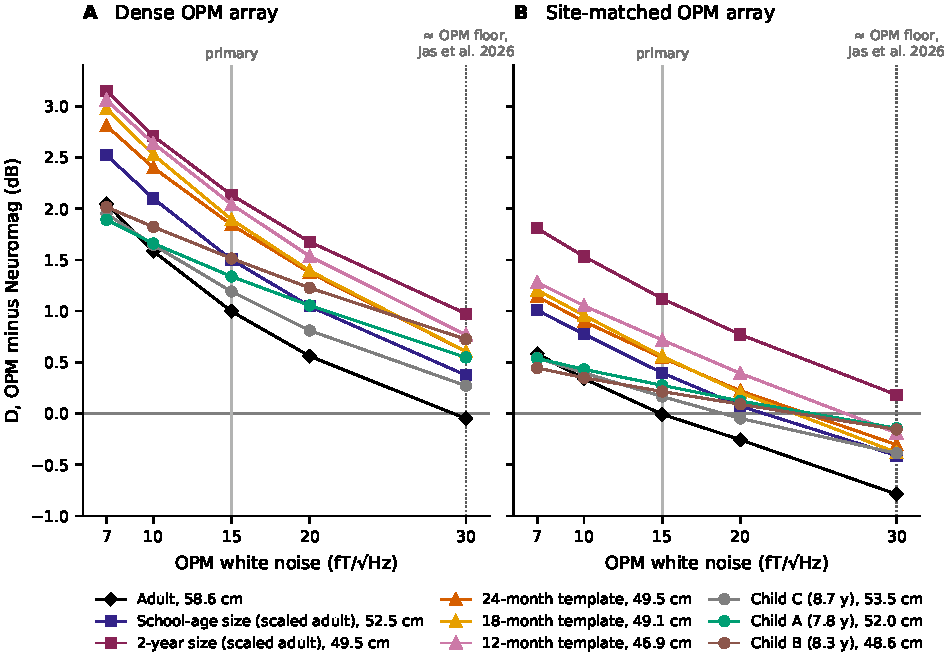
\includegraphics[width=\textwidth]{Figure_S11.pdf}
\caption{The OPM noise level across heads. $D$ (fixed adult helmet at top contact) against the OPM's white sensor noise (7, 10, 15, 20 and 30 fT/√Hz), Neuromag's noise unchanged, for the adult and the eight smaller heads. (A) Dense OPM array. (B) Site-matched OPM array. Solid vertical line: the primary 15 fT/√Hz; dotted line: 30 fT/√Hz, about the OPM empty-room floor read from the spectra of \citet{jas2026}, a broadband value not matched to the 1–40 Hz band.}\label{fig:S11}
\end{figure}

\section{The spike study: design, results and localization}\label{sec:S7}

\subsection{The exploratory design}\label{sec:S7.1}

The detection study ran the noise model in the time domain, with each component scaled so that its in-band covariance equaled that of the adult model and the room field not projected out (Table~\ref{tab:S18}). The spike was the spike-wave complex of \citet{hunold2016}, digitized, stretched in time by 0.75, 1 and 1.5 (3 morphologies) and passed through the band-pass filter of the data.

Spikes were placed at 72 locations stratified by depth below the scalp (10–20, 20–30, 30–45 and 45–70 mm; 18 locations per band) and by orientation (3 bands from radial to tangential; 6 locations per depth and orientation stratum). Each location received 18 focal-dipole events, at 6 strengths of 10, 20, 40, 80, 160 and 320 nAm, each with every morphology, and patch events of 10 mm radius carrying the same total moments with the unstretched morphology. This gave 1,296 focal and 432 patch events, 1,728 per anatomy, injected in random order and identically in every array. The adult's locations lay 24 in the frontal lobe, 14 in the parietal, 14 in the temporal, 12 in the cingulate, 6 in the insula and 2 in the occipital lobe, at median depths of 16.9, 26.0, 36.8 and 51.7 mm in the four bands.

Every array, Neuromag and the dense and site-matched optically pumped magnetometer (OPM) arrays, was read by two detectors, and Neuromag also by its magnetometers and by its gradiometers alone (5 sensor sets per anatomy). Both detectors whitened the data with a Ledoit--Wolf covariance \citep{ledoit2004} estimated from null data and filtered them with the spike templates. The oracle detector tests the whitened, template-filtered projection on the true field pattern at the true peak (one-sided; per-trial false-positive probability 0.001).

The practical detector takes at every sample the largest normalized output over the templates and the candidate field patterns of a cortical grid that excludes the true sources (Table~\ref{tab:S18}), and its local maxima at least 0.25 s apart are events. A spike counts as detected when an event above threshold lies within ±50 ms of its peak; the same events count as false on null data. Like the oracle, it uses the simulated morphologies and the true forward model (main text, Section 2.5). Whether it is equally idealized for every array was not tested in the exploratory run; the pre-specified run's mismatch variant tests one departure (Section~\ref{sec:S7.5}), and focal on-scalp patterns may be more sensitive to forward-model and coregistration error.

Its thresholds for 1 false event per minute were set on independent null data and frozen; on held-out null data they gave 0.40–1.55 false events per minute across sensor sets and anatomies (Table~\ref{tab:S9}). In the adult, the practical detector needed 1.83–2.08 times the oracle's strength for half detection at 10–20 mm.

\begin{table}[tbp]
\caption{Held-out false-event rates of the exploratory run. False events per minute of the practical detector on 20 min of held-out null data, at thresholds frozen for 1 false event per minute on 20 min of calibration null data.}\label{tab:S9}
\centering\footnotesize
\begin{tabular}{lccc}
\toprule
Head & Neuromag (306 channels) & Site-matched OPM array & Dense OPM array \\
\midrule
Adult & 1.30 & 0.70 & 0.95 \\
School-age size & 1.40 & 0.50 & 1.05 \\
2-year size & 0.40 & 0.65 & 1.20 \\
24-month template & 0.70 & 1.55 & 1.30 \\
18-month template & 0.90 & 1.45 & 1.10 \\
12-month template & 1.20 & 0.95 & 0.85 \\
Child A & 0.90 & 1.35 & 0.75 \\
Child B & 0.80 & 1.55 & 0.70 \\
Child C & 1.20 & 0.70 & 0.75 \\
\bottomrule
\end{tabular}
\tablenotes{OPM, optically pumped magnetometer. The adult sits at its measured head position, the other heads at top contact in the fixed adult helmet.}
\end{table}

A band's S50 pools its 324 focal events, the morphologies over its 18 locations; patch events enter neither S50 nor the paired tests. The paired ratio S50\textsubscript{Neuromag}/S50\textsubscript{OPM} is above 1 when the OPM array needs less strength (Section~\ref{sec:S1}), and interval bounds printed as 1.00 are classed by their unrounded values throughout. The adult sat at its measured pose and the smaller heads at top contact (main text, Section 2.5), so the adult's spike results are not placed by the same rule as theirs.

The exploratory spike endpoint, chosen after the analyses (Section~\ref{sec:S8.2}), was the dense array against Neuromag's 306 channels in the 10–20 mm band with the practical detector. It was tested with the two-sided exact sign-flip test on per-location differences in detection counts, Holm-adjusted \citep{holm1979} over the 9 anatomies, with the paired S50 ratio and its location-bootstrap interval as the effect size. This band, array and detector were chosen from the 24 comparisons per OPM array of each anatomy, a selection that the correction over anatomies does not control. The detection family has 48 comparisons per anatomy: two OPM arrays against Neuromag's 306 channels, its gradiometers and its magnetometers, with both detectors, in 4 depth bands. The localization family has 40: two OPM arrays; focal and patch sources at two strengths; and the dipole error, the two errors of dynamic statistical parametric mapping (dSPM), and joint detection and localization with the study's dSPM or with the dipole.

The sign-flip test uses the locations whose difference in detection counts is not zero, and p is smallest when all of them favor one array. With a band's 18 locations that smallest p is 7.6 $\times 10^{-6}$, and p < 0.05 needs at least 6 such locations. With equal differences the test is the exact sign test: of 18 locations, 14 must then favor one array for p < 0.05 (p = 0.031; with 13, p = 0.096), and 16 for the first Holm step over 9 anatomies, p < 0.0056 (p = 0.0013). Of the pre-specified 36 locations (12 per orientation stratum), 25 are needed (p = 0.029) and 27 for the first Holm step (p = 0.0039).

Unequal differences can move p either way: the adult's 11 locations favoring the OPM against 1 favoring Neuromag gave p = 0.0039, against 0.0063 had the differences been equal. Beyond 20 non-zero locations the run estimated p from 20,000 random sign patterns (resolution 5 $\times 10^{-5}$); the p values reported for the pre-specified run are exact (Section~\ref{sec:S7.5}). These values follow from the design alone; power and a minimal detectable S50 ratio depend on how detection varies between locations and were not computed. The pilot runs that prompted doubling the locations to 36 (child A, 18 locations, test seeds; main text, Section 2.5) do not estimate power either, and their outputs were not kept; the pre-specified declaration describes 18 locations as underpowered, a reading we do not adopt.

\subsection{Results of the exploratory run}\label{sec:S7.2}

The exploratory run had one noise realization per event and an endpoint chosen after the analyses; it is superseded as evidence by the pre-specified run (main text, Section 3.6; Section~\ref{sec:S7.5}). Every anatomy's S50 point estimate favored the dense array 10–20 mm below the scalp (Fig.~\ref{fig:S12}A; Table~\ref{tab:S10}), and so did the per-location counts under a Holm correction over the 9 anatomies (largest adjusted p 0.022, child A, whose S50 interval spans 1). The anatomies are not independent replications.

Table~\ref{tab:S10} sets the oracle's S50 ratio, the quantity most directly tied to the detectability metric, beside the practical detector's. The oracle's ratios were the larger in 7 of the 9 anatomies (not in the 18-month template and child C), as expected where the oracle's advantage is not diluted by the scan over times and candidates. The adult's detection curves are shown in Fig.~\ref{fig:S13}.

\begin{sidewaystable}
\caption{Detection of simulated spikes 10–20 mm below the scalp in the exploratory run. Practical detector with thresholds frozen at 1 false event per minute, 18 locations per anatomy. The endpoint was chosen after the analyses.}\label{tab:S10}
\centering\footnotesize
\begin{tabularx}{\linewidth}{L{3.0cm}L{2.0cm}YL{2.2cm}L{1.4cm}L{1.4cm}YY}
\toprule
Head & S50 (nAm), Neuromag / dense & Ratio, dense & Locations, OPM / Neuromag & p & Holm p & Ratio, site-matched & Ratio, dense, oracle \\
\midrule
Adult & 47 / 34 & 1.36 [1.10, 1.58] & 11 / 1 & 0.0039 & 0.015 & 1.16 [0.88, 1.44] & 1.55 [1.22, 1.74] \\
School-age size & 53 / 33 & 1.60 [1.31, 1.87] & 13 / 0 & 0.00024 & 0.0017 & 1.27 [0.99, 1.52] & 1.62 \\
2-year size & 61 / 37 & 1.65 [1.41, 1.87] & 17 / 0 & <0.0001 & 0.00014 & 1.60 [1.21, 1.82] & 1.69 \\
24-month template & 43 / 30 & 1.44 [1.20, 1.65] & 14 / 2 & 0.0015 & 0.0076 & 1.22 [1.00, 1.42] & 1.51 \\
18-month template & 36 / 27 & 1.33 [1.16, 1.62] & 16 / 0 & <0.0001 & 0.00024 & 1.10 [1.02, 1.28] & 1.30 \\
12-month template & 43 / 29 & 1.46 [1.21, 1.84] & 14 / 1 & 0.00049 & 0.0029 & 1.28 [1.09, 1.46] & 1.89 \\
Child A & 61 / 48 & 1.27 [0.93, 1.63] & 11 / 4 & 0.022 & 0.022 & 1.05 [0.75, 1.40] & 1.53 \\
Child B & 65 / 55 & 1.18 [1.02, 1.51] & 12 / 3 & 0.0085 & 0.017 & 1.06 [0.87, 1.35] & 1.31 \\
Child C & 52 / 36 & 1.43 [1.06, 1.62] & 14 / 2 & 0.0037 & 0.015 & 1.08 [0.92, 1.31] & 1.36 \\
\bottomrule
\end{tabularx}
\tablenotes{S50: strength for half detection (Neuromag 306 channels / dense OPM array). Ratio: paired S50 ratio Neuromag/OPM with its bootstrap interval over locations. Locations: those with more events detected by the OPM / by Neuromag. p: exact sign-flip test on per-location differences in detection counts, uncorrected and Holm-adjusted over the anatomies. Oracle: the paired S50 ratio of the dense array with the oracle detector. OPM, optically pumped magnetometer.}
\end{sidewaystable}

\begin{figure}[tbp]
\centering
\captionsetup{font=footnotesize}
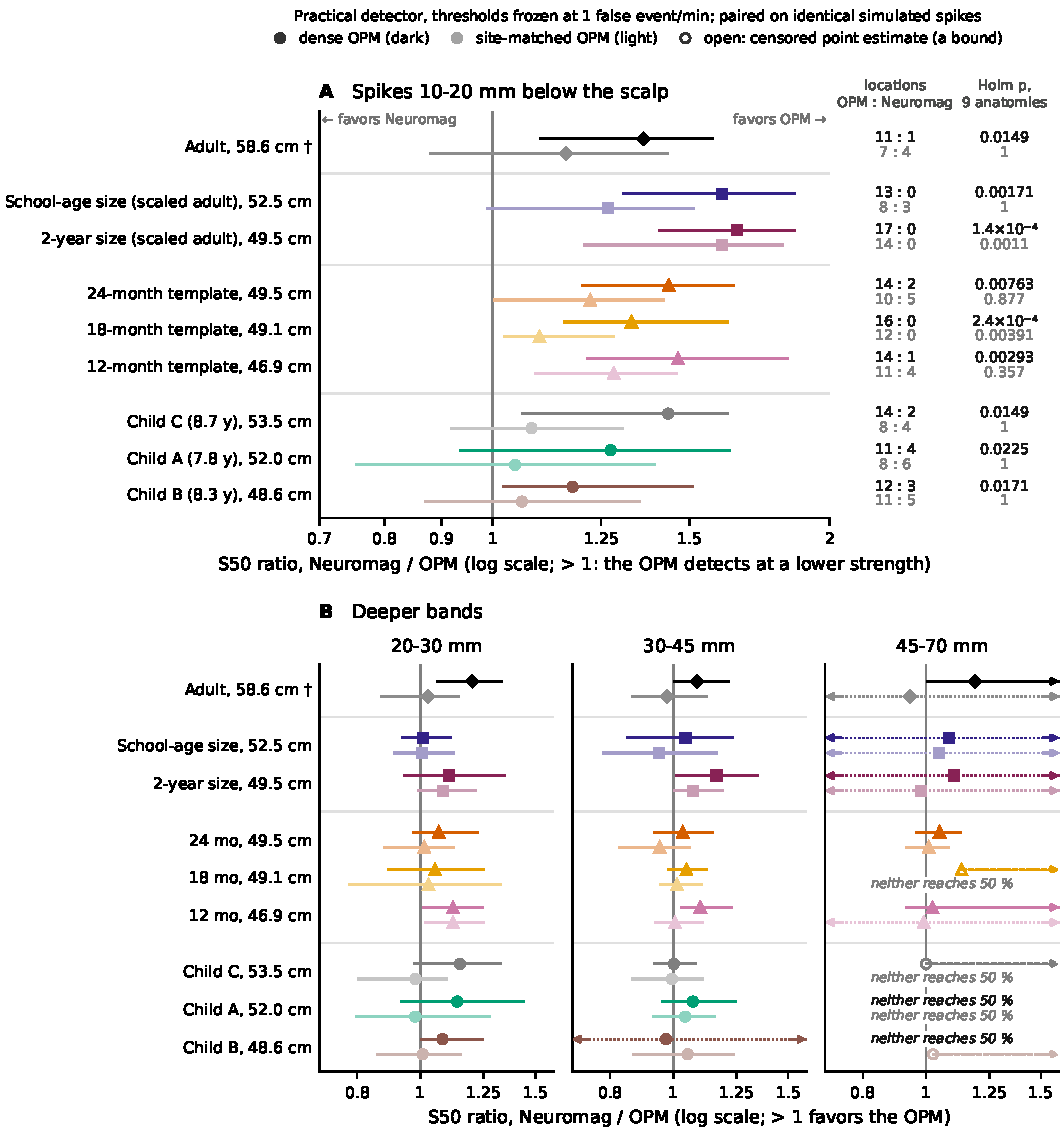
\includegraphics[width=\textwidth,height=0.55\textheight,keepaspectratio]{Figure_S12.pdf}
\caption{Simulated interictal spikes, exploratory run. Paired S50 ratio Neuromag (306 channels) / OPM, practical detector; logarithmic axis with a line at 1 (above 1: the OPM detects at a lower strength). (A) Spikes 10–20 mm below the scalp, with the locations favoring each system and the sign-flip p Holm-adjusted over the 9 anatomies for each array separately; this endpoint was chosen after the analyses. (B) The deeper bands. Dark markers: dense OPM array; light markers: site-matched OPM array. Lines: 95\,\% bootstrap intervals over the 18 locations per band and anatomy (324 focal events). Arrows: open interval ends (resamples outside the tested 10–320 nAm); dotted lines: intervals open at both ends; open markers: censored point estimates (with a dashed arrow: Neuromag does not reach half detection, so the ratio lies above the bound); ``neither reaches 50\,\%'': no estimate. Dagger: the adult at its measured head position; other heads at top contact. OPM, optically pumped magnetometer.}\label{fig:S12}
\end{figure}

\begin{figure}[tbp]
\centering
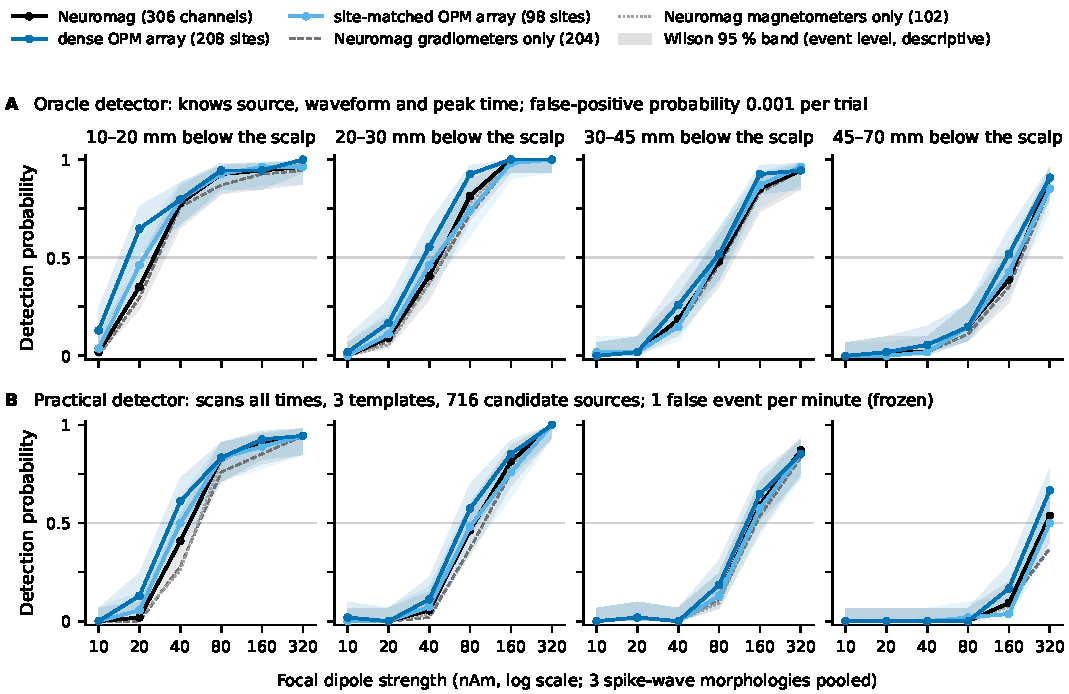
\includegraphics[width=\textwidth]{Figure_S13.pdf}
\caption{Detection curves of the adult, exploratory run. Probability of detecting a focal spike against its strength (10–320 nAm, logarithmic axis; 54 events per point: 18 locations and 3 morphologies pooled) in the four depth bands, for Neuromag (306 channels), the dense OPM array (208 sites) and the site-matched OPM array (98 sites), with Neuromag's gradiometers (dashed) and magnetometers (dotted) alone as secondary comparators. (A) The oracle detector (false-positive probability 0.001 per trial). (B) The practical detector (3 templates, 716 candidate sources, 1 false event per minute); on the held-out null data its frozen thresholds gave 1.20 and 0.65 false events per minute for the gradiometers and magnetometers (arrays: Table~\ref{tab:S9}). Shaded: Wilson 95\,\% intervals at the event level, descriptive only, because the events of a point share locations. Gray horizontal line: half detection. At 10–20 mm the strength for half detection is 16, 22 and 25 nAm with the oracle and 34, 40 and 47 nAm with the practical detector (dense, site-matched, Neuromag). OPM, optically pumped magnetometer.}\label{fig:S13}
\end{figure}

A Bonferroni correction over the 24 comparisons per OPM array from which the endpoint was chosen (threshold 0.0021) is the stricter test. Of the nine anatomies, five passed it, the scaled adults and the templates, while the adult (p = 0.0039) and the three children did not. Over all 48 comparisons per anatomy (threshold 0.0010), 4 passed.

Because the frozen thresholds gave unequal false-event rates on the held-out null data (Table~\ref{tab:S9}), every detector's threshold was also reset to 1 false event per minute on those data and the stored simulations were re-evaluated. Fitted and evaluated on the same data, this check is in-sample for the rate and does not establish equal operating points on new data; the pre-specified run uses separate evaluation null data for that. The dense array's ratios at 10–20 mm stayed above 1 in every anatomy (1.21–1.63). In the adult the ratio was 1.40 [1.12, 1.59] (12 locations favoring the OPM, 1 Neuromag, p = 0.0022), against 1.36 at the frozen thresholds.

The site-matched array's S50 interval lay above 1 in 4 anatomies, but its detection counts differed (uncorrected p < 0.05) in only 2, the 2-year size control and the 18-month template, and not in the adult (p = 0.40) or any child.

Deeper spikes leaned the same way less consistently (Fig.~\ref{fig:S12}B). The location counts favored the dense array in 25 of the 27 deeper band-and-anatomy cells (1 tie, 1 against), and the S50 point estimates at 20–30 mm were above 1 in 9 of 9 anatomies. Of the 6 cells with p < 0.05, 6 favored the OPM, and none survived that Bonferroni correction. With the endpoint's rule, a Holm correction over the anatomies band by band, 1 survived: the adult's 45–70 mm band (adjusted p 0.035). Which deeper cells reach p < 0.05 varied between model versions (Section~\ref{sec:S8.2}).

Of the adult's 324 superficial focal events (54 per strength), 19 were detected only by the dense array (6, 12 and 1 at 20, 40 and 160 nAm) and 1 only by Neuromag (at 40 nAm). The dense array and Neuromag detected 7 and 1 events at 20 nAm and 33 and 22 at 40 nAm, and nearly the same numbers from 80 nAm up (45 and 45, 50 and 49, 51 and 51). The OPM's gain was thus concentrated on weak superficial spikes; its weight in a clinical recording depends on how many real discharges are that weak, which the design's strength grid cannot tell.

At the adult's 18 locations of each band, the dense array's median detectability ratio was 1.45, 1.16, 1.09 and 1.05 from the shallowest to the deepest band, and the oracle's paired S50 ratio 1.55, 1.29, 1.09 and 1.20. The two agreed in direction in every band, and closely at 30–45 mm. The oracle ratio exceeded the detectability ratio most in the deepest band, whose interval ([1.00, 1.42]) lies just above 1 because few events are detected at the lower strengths and S50 is interpolated from them. Exact agreement is not expected, because the detectability ratio is a median of per-location ratios whereas the S50 ratio pools the band's detection curves. The oracle is the better-behaved of the two spike quantities, and the pre-specified run reports it beside the practical detector (Table~\ref{tab:S11}).

\subsection{Localization}\label{sec:S7.3}

Localization was examined at 24 locations with focal and patch sources of 80 and 320 nAm, one event per source type and strength at each location (24 per condition, unstretched morphology), in independent null data. The inverse used a single-compartment boundary-element model (BEM), whereas the simulation used three layers, and one of 8 coregistration-error draws of 2 mm and 2° per location, the same for every array. This error displaced the adult's sources by a median of 2.9 mm, and by 2.1–3.2 mm over the anatomies. The noise covariance was a Ledoit--Wolf estimate from 5 min of null data, and the source grid had fixed orientations at 5-mm spacing (2,114–3,821 sources) and excluded the true source vertices.

Equivalent current dipoles (ECDs) were fitted with MNE-Python \citep{gramfort2013} at least 5 mm inside the inner skull. dSPM \citep{dale2000}, with depth weighting 0.8 and a regularization set by an assumed signal-to-noise ratio (SNR) of 3, was computed in the study's implementation and in MNE-Python's, at the true peak sample. The error is the distance from the true source (a patch's center) to the dipole or to the dSPM peak, read on the MRI through the perturbed transform. Joint success is detection by the practical detector (thresholds for 1 false event per minute from 10 min of null data) with an error of at most 10 mm. Paired error differences were tested with the Wilcoxon signed-rank test and joint success with an exact McNemar test.

Both dSPM implementations use fixed orientations on the same grid, the same noise covariance, a depth exponent of 0.8, $\lambda^{2}$ = 1/9, a source covariance scaled to the whitened rank and dSPM normalization. They differ in the depth weighting. The study's implementation uses the whitened gains of all of an array's channels, without a limit. MNE-Python's is limited at its default of 10 and uses the unwhitened gains of the gradiometers, or of the magnetometers where there are none (the OPM arrays). Both are reported, because the paired dSPM differences depend on this choice.

Dipole fits of detected 320-nAm focal spikes had median errors of 3.7–7.6 mm in every array and anatomy. Of 360 paired comparisons, 65 had p < 0.05, where 18 would be expected by chance. Most concerned dSPM errors (21 with the study's implementation, 27 with MNE-Python's); 6 concerned dipole errors and 11 joint detection and dSPM localization within 10 mm. Of these, 61 favored an OPM array, 3 had a zero median difference and 1 favored Neuromag. Of the 65, 28 concerned mostly undetected 80-nAm sources, and the two dSPM implementations share their events.

In all, 8 comparisons survived a Bonferroni correction within anatomy and array, 6 of them at 80 nAm, where most sources go undetected, and 0 survived one over all 360. The adult's dSPM gain for 320-nAm patches depended on the implementation: −5.6 mm (p = 0.054) with the study's estimator and −1.0 mm (p = 0.22) with MNE-Python's.

Of the 216 paired error differences in Fig.~\ref{fig:S14}, 54 had p < 0.05 (6 for the dipole fit, 27 for MNE-Python's dSPM, 21 for the study's), and eight of these fell below 0.0025, the Bonferroni threshold for the 20 comparisons of one anatomy and OPM array. At 80 nAm all 108 estimates rest mostly on undetected events, whose errors are those of noise.

Of the 216 medians, 20 were exactly zero, because the dSPM peaks of both systems often fall on the same vertex of the shared 5-mm grid, and 30 were positive (Neuromag closer). The errors include every event, detected or not, because selecting on detection would select on each system's own noise. For joint detection and localization within 10 mm (Fig.~\ref{fig:S15}), of the 72 paired comparisons per method, 0 with the dipole fit and 11 with the study's dSPM had p < 0.05 (exact McNemar, uncorrected), all favoring the OPM array; none survived a correction. Joint success assumes the event time is known, because localization is read at the true peak sample.

Every event received a dipole. Under declared criteria, a dipole or dSPM error above 30 mm is gross, and a dipole confidence volume above 10 cm³ is unconstrained. Over the 864 events per system, Neuromag had 332 gross dipole errors (27 among its 456 detected events), the dense array 310 (44 among 501) and the site-matched array 325 (38 among 475), that is, 5.9–8.8\,\% of detected events. Gross errors of the study's dSPM among detected events numbered 77 for Neuromag (17\,\%), 39 for the dense array (7.8\,\%) and 36 for the site-matched array (7.6\,\%).

Of all gross errors (dipole and the study's dSPM, three arrays), 87\,\% belonged to undetected events and 73\,\% to 80-nAm events. The denominators differ between arrays because each array detects different events, so these rates are described, not compared. No localization difference was established in any anatomy.

\begin{figure}[p]
\centering
\captionsetup{font=footnotesize}
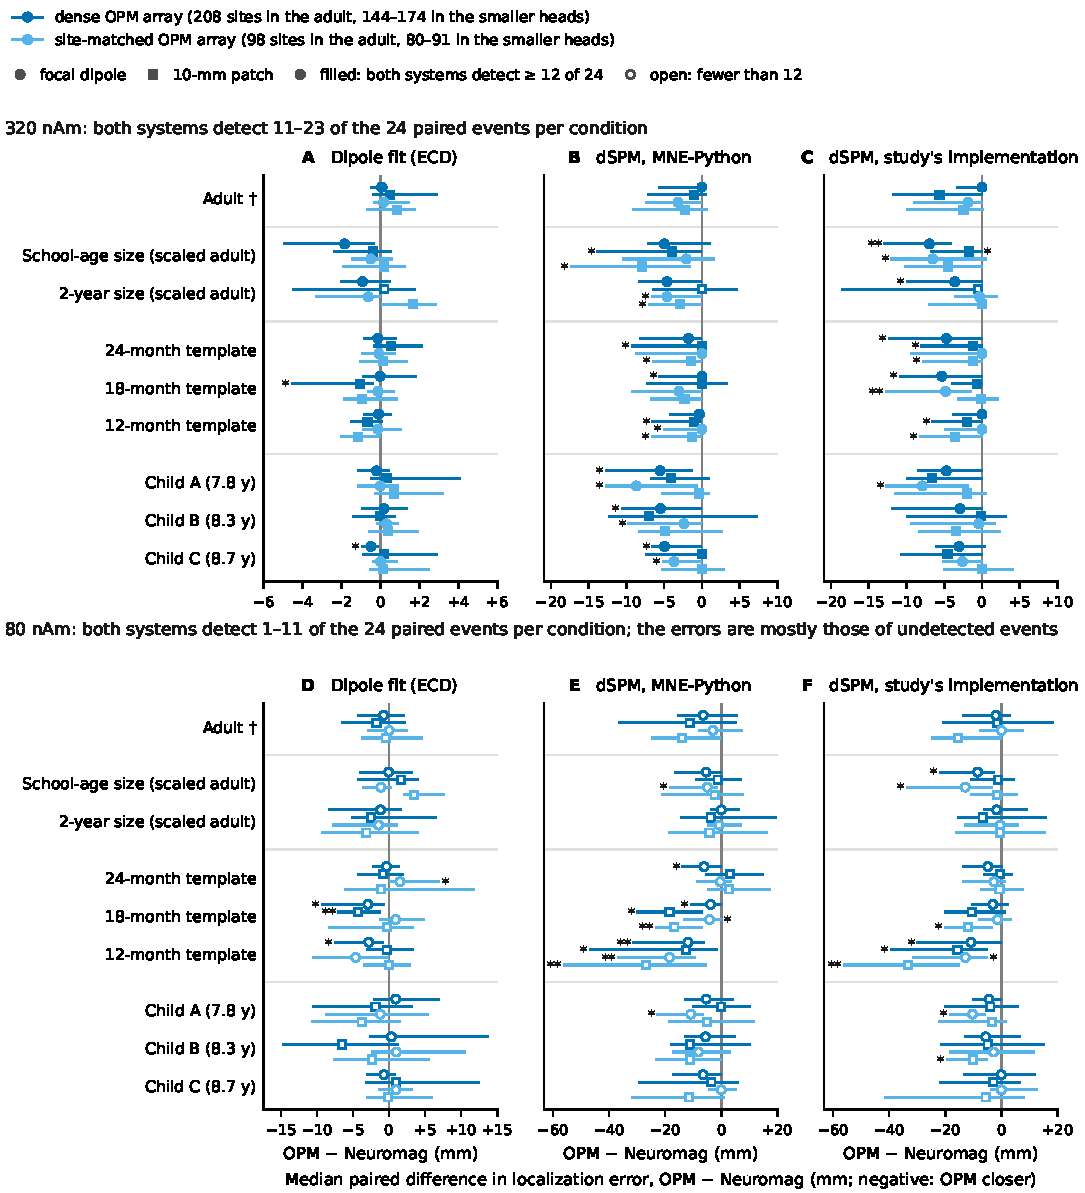
\includegraphics[width=\textwidth]{Figure_S14.pdf}
\caption{Localization effect sizes, exploratory run. Median over the 24 events of a condition of the paired difference in localization error, OPM array minus Neuromag (306 channels), with 95\,\% bootstrap intervals over events (2,000 resamples); negative: the OPM array localizes closer to the true source. (A, D) Equivalent-current-dipole (ECD) fit. (B, E) dSPM through MNE-Python. (C, F) dSPM through the study's implementation. (A--C) 320 nAm. (D--F) 80 nAm, where the errors are mostly those of undetected events. Colors and marker shapes as in the key; filled markers: both systems detected at least half of the events (practical detector); open markers: fewer. Stars: uncorrected Wilcoxon signed-rank p < 0.05 (one) and p < 0.0025, the Bonferroni threshold over the 20 comparisons of one anatomy and OPM array (two). The x axes differ between strengths and between the dipole and dSPM columns. Dagger: the adult at its measured head position; other heads at top contact. dSPM, dynamic statistical parametric mapping; OPM, optically pumped magnetometer.}\label{fig:S14}
\end{figure}

\begin{figure}[p]
\centering
\captionsetup{font=footnotesize}
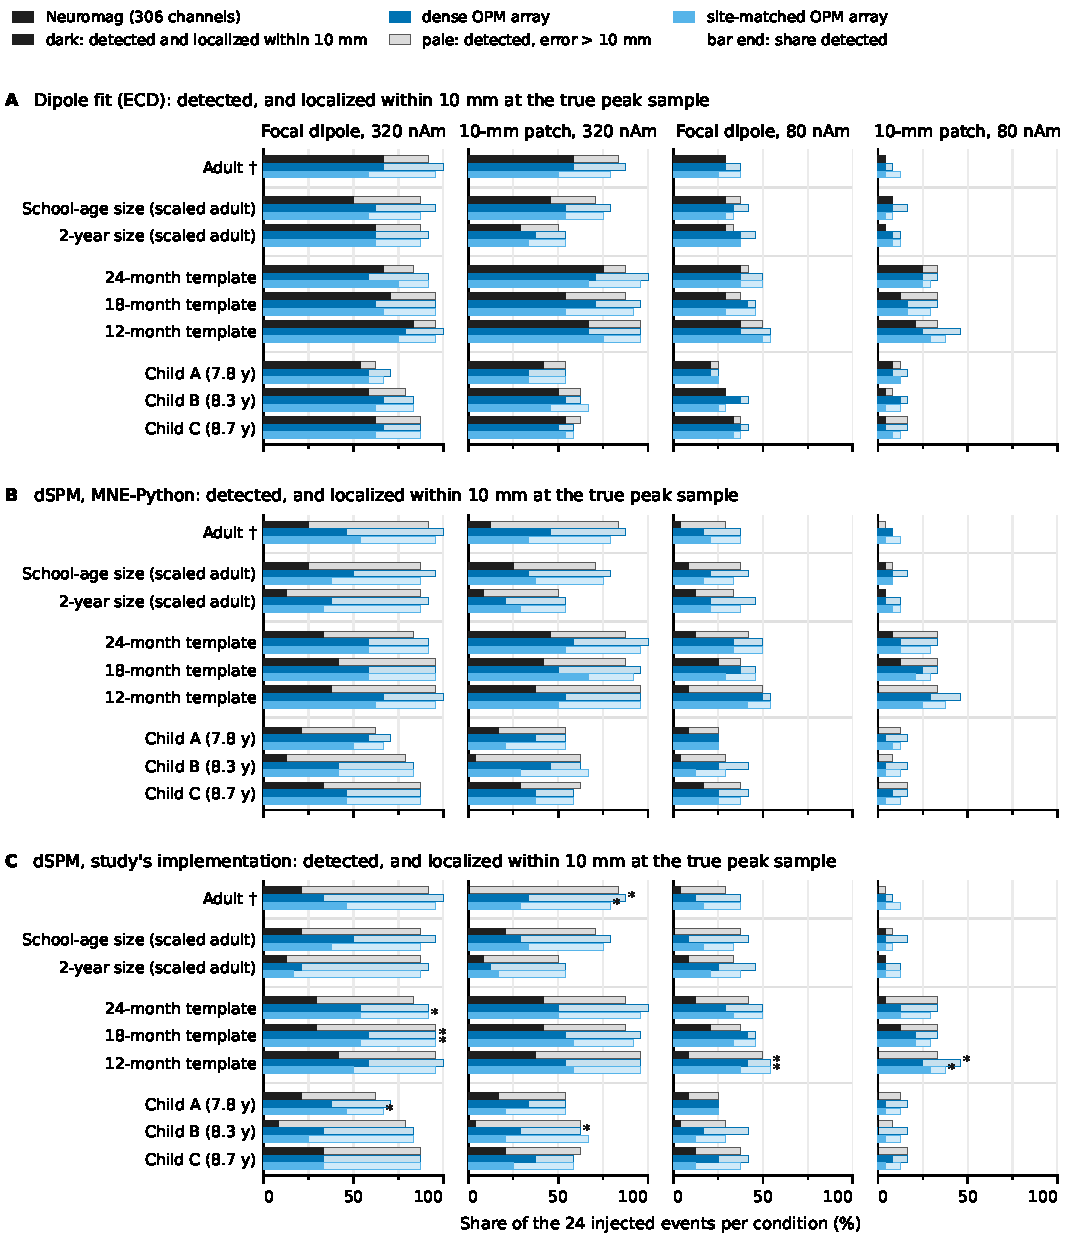
\includegraphics[width=\textwidth]{Figure_S15.pdf}
\caption{Joint detection and localization, exploratory run. For each anatomy, system and condition (focal dipole or 10-mm patch at 320 and 80 nAm), the bar's end is the share of the 24 injected events detected by the practical detector; its dark part is the share both detected and localized within 10 mm, its pale part the share detected but localized farther away. (A) Equivalent-current-dipole (ECD) fit. (B) dSPM through MNE-Python. (C) dSPM through the study's implementation. Stars: OPM minus Neuromag difference in joint success with p < 0.05 (exact McNemar, uncorrected; dipole fit and the study's dSPM only). The frozen thresholds gave 0.2–1.9 false events per minute on the localization study's held-out null data over the nine anatomies and three systems. Dagger: the adult at its measured head position; other heads at top contact. dSPM, dynamic statistical parametric mapping; OPM, optically pumped magnetometer.}\label{fig:S15}
\end{figure}

\subsection{Head motion}\label{sec:S7.4}

Head motion and slippage of the OPM cap were bounded rather than simulated in time, on the adult and the 24- and 12-month templates at top contact: the head was displaced in the fixed helmet by up to 10 mm or rotated about the head origin, and the dense OPM cap was rotated on the head by up to 3°, lifting sensors that would enter the scalp. Each case was evaluated with the matched filter of the reference geometry (uncompensated) and with the displaced geometry known. A sustained 10-mm drop in the fixed helmet cost Neuromag 1.64–1.72 dB uncompensated and 0.36–0.39 dB with the displaced geometry known, the latter comparable to an uncompensated 3° slip of the OPM cap (0.12–0.46 dB). A 60-s time course of exact rigid motion checked the field-artifact model only; motion in the spike simulations, and its interaction with detection thresholds, was not simulated.

\subsection{The pre-specified run}\label{sec:S7.5}

\begin{sidewaystable}
\caption{The pre-specified spike run per head. Focal spikes 10–20 mm below the scalp at 36 newly drawn locations per anatomy (648 focal events of 10–320 nAm; the first of 5 noise replicates).}\label{tab:S11}
\centering\footnotesize
\begin{tabularx}{\linewidth}{L{3.2cm}L{1.7cm}YL{1.9cm}L{1.3cm}YYL{4.4cm}}
\toprule
Head & S50 (nAm), Neuromag / dense & Ratio, dense & Locations, OPM / Neuromag & Holm p & Oracle, ratio & Mismatch, ratio & Site-matched, ratio (Holm p) \\
\midrule
Adult & 50 / 35 & 1.45 [1.21, 1.68] & 24 / 0 & <0.0001 & 1.39 [1.22, 1.55] & 1.50 [1.30, 1.67] & 1.30 [1.10, 1.46] (0.035) \\
School-age size & 45 / 31 & 1.44 [1.26, 1.58] & 25 / 1 & <0.0001 & 1.61 [1.46, 1.76] & 1.39 [1.23, 1.52] & 1.28 [1.10, 1.43] (0.048) \\
2-year size & 54 / 37 & 1.47 [1.24, 1.62] & 27 / 1 & <0.0001 & 1.62 [1.40, 1.78] & 1.49 [1.26, 1.67] & 1.16 [1.05, 1.35] (0.0031) \\
24-month template & 35 / 27 & 1.28 [1.18, 1.45] & 28 / 2 & <0.0001 & 1.51 [1.31, 1.84] & 1.42 [1.26, 1.68] & 1.06 [0.95, 1.17] (0.067) \\
18-month template\textsuperscript{a} & 41 / 29 & 1.43 [1.26, 1.61] & 30 / 1 & <0.0001 & 1.62 [1.41, 1.90] & 1.44 [1.25, 1.65] & 1.30 [1.15, 1.48] (<0.0001) \\
12-month template & 41 / 29 & 1.39 [1.25, 1.56] & 29 / 1 & <0.0001 & 1.48 [1.30, 1.84] & 1.43 [1.25, 1.60] & 1.30 [1.15, 1.48] (0.0084) \\
Child A & 51 / 40 & 1.27 [1.07, 1.38] & 14 / 3 & 0.010 & 1.29 [1.09, 1.52] & 1.23 [1.06, 1.41] & 0.99 [0.84, 1.14] (1.0) \\
Child B & 57 / 42 & 1.35 [1.15, 1.56] & 21 / 2 & <0.0001 & 1.27 [1.11, 1.52] & 1.23 [1.02, 1.48] & 1.08 [0.99, 1.20] (1.0) \\
Child C & 50 / 39 & 1.30 [1.15, 1.43] & 25 / 2 & <0.0001 & 1.34 [1.17, 1.55] & 1.34 [1.18, 1.50] & 1.10 [1.00, 1.27] (0.15) \\
\bottomrule
\end{tabularx}
\tablenotes{\scriptsize S50: strength for 50\,\% detection, Neuromag (306 channels) / dense OPM array, in whole nAm (the ratios use the unrounded values). Ratio: S50\textsubscript{Neuromag}/S50\textsubscript{OPM}, a ratio of the two location-pooled estimates with its 95\,\% interval from paired location resampling (1,000 resamples); above 1, the OPM detects at a lower strength. Locations: those at which the OPM / Neuromag detected more events (the others are ties). Holm p: exact two-sided sign-flip test on the per-location differences in detection counts, Holm-adjusted over the nine anatomies within each column's family; ``<0.0001'': an exact p below the printed precision. Interval bounds printed as 1.00 are classed by their unrounded values (child C's site-matched interval, printed [1.00, 1.27], has the lower bound 0.9997 and spans 1). OPM, optically pumped magnetometer. \textsuperscript{a}The 18-month template is classed misregistered by the MRI check (a possibly misaligned white surface, or the weak contrast of an average image; main text, Section 2.2).}
\end{sidewaystable}

The pre-specified run (main text, Sections 2.5 and 3.6; Fig. 10) is summarized in Table~\ref{tab:S11}, whose dense-array columns with the practical detector are the declared endpoint (thresholds frozen for a nominal 1 false event per minute); the oracle, mismatch and site-matched columns are secondary.

The declaration fixed seven elements, and the run followed it at a single code version, complete in all nine anatomies. First, every random stream was spawned from the root seed 20261005 by anatomy and purpose (10 purposes), and the noise replicates of an event from its event stream; only the random sign patterns of the sign-flip test use the fixed seed 0 of the test's implementation, in every anatomy, family and replicate (Table~\ref{tab:S17}). Second, 36 locations per anatomy were newly drawn in the 10–20 mm band (12 in each of the 3 orientation strata), vertex-disjoint from the exploratory ones where a stratum allows. The pools of 109–2,249 candidate vertices per stratum excluded the 72 exploratory locations, so no stratum shared a vertex; the nearest exploratory location lay 2.7 mm away at the closest and a median 13.6–18.6 mm away over the anatomies.

The locations' median depth was 12.9–17.4 mm; the adult's lay 17 in the frontal lobe, 10 in the parietal, 8 in the temporal and 1 in the occipital lobe. Each location received 18 focal events per replicate (6 strengths of 10–320 nAm, morphologies stretched by 0.75, 1 and 1.5): 648 events per replicate, 3,240 per anatomy and 29,160 in all. Third, the test is the two-sided sign-flip test, exact up to 20 non-zero location differences and otherwise estimated from 20,000 random sign patterns. Fourth, the effect size is the paired S50 ratio with a location-bootstrap interval of 1,000 resamples.

Where the run estimated a sign-flip p (resolution 5 $\times 10^{-5}$), the estimate was zero if no sampled pattern reached the observed statistic. Because the differences are integer counts, the exact p over all $2^{n}$ sign patterns follows from the distribution of the signed sum. We computed it from the stored differences for all 540 cells of anatomy and comparison, reproducing exactly the 47 cells that the run had enumerated itself, and every p reported here and in the main text is this exact value. The run's estimates differ from it by at most 0.0073 and give the same Holm decision for every anatomy in all 25 families; where an estimate was zero, the exact Holm-adjusted value reaches 0.00040. Before the run, the pre-specified endpoint code, applied to the exploratory run's stored states, reproduced its location counts, p values and S50 ratios exactly in all 36 comparisons (nine anatomies, both OPM arrays, both detectors).

Fifth, separate null segments served the whitener (10 min), the threshold fit (20 min; 20 events above each frozen threshold), the held-out check (20 min) and the evaluation of the false-event rates of the frozen and the rate-matched thresholds (20 min), 70 min in all. Sixth, each event has 5 noise replicates, the first carrying the endpoint and the others measuring Monte Carlo variability. The practical detector's dictionary held 452–728 candidate patterns over the anatomies, and the oracle's realized per-trial false-positive probability on the held-out null was 0.00093–0.0011 over the anatomies and arrays, against the declared 0.001.

Seventh, the declared mismatched detector's templates sit at the geometric midpoints of the injected stretches (0.87 and 1.22: 2 templates), each injected morphology lying 13–18\,\% away from the nearest template. Its candidate patterns come from a single-compartment BEM, and one coregistration error per anatomy (2 mm, 2°), shared by all arrays, displaced the candidate dictionary by a median of 1.6–4.9 mm at the spike locations over the anatomies (0.7–5.9 mm over all locations). Its thresholds were set for a nominal 1 false event per minute on the calibration null and frozen and, like the primary detector's, re-fitted on the held-out null as a secondary analysis.

In each of the five Monte Carlo replicates the endpoint passed in all nine anatomies (45 of 45 anatomy-replicate cells; Table~\ref{tab:S12}). Over the replicates the ratio ranged from 1.15 to 1.49, with an SD within an anatomy of 0.041–0.089 in log\textsubscript{2} units (in percent: main text, Section 3.6; Table~\ref{tab:S12}). Pooled over the replicates (3,240 events per anatomy), the Holm-adjusted p was at most 0.0013. The oracle's pooled ratios were 1.35–1.60 and the mismatched detector's 1.23–1.45, each family passing in all nine anatomies. The pre-specified ratio was 0.89–1.14 times the exploratory one, below it in 6 of the 9 anatomies, and the exploratory point estimate lay within the pre-specified interval in 6.

\begin{sidewaystable}
\caption{Replicates of the pre-specified endpoint. The declared endpoint in every noise replicate: dense OPM array against Neuromag's 306 channels, practical detector, thresholds frozen for a nominal 1 false event per minute, focal spikes 10–20 mm below the scalp at 36 locations per anatomy.}\label{tab:S12}
\centering\footnotesize
\begin{tabularx}{\linewidth}{L{3.0cm}L{4.6cm}L{1.0cm}L{1.3cm}L{2.0cm}YL{1.8cm}L{1.4cm}}
\toprule
Head & Ratio per replicate & SD (\%) & Largest p & Pre-specified / exploratory & Pooled ratio & Pooled locations, OPM / Neuromag & Pooled Holm p \\
\midrule
Adult & 1.45, 1.46, 1.36, 1.39, 1.41 & 2.9 & <0.0001 & 1.06 & 1.41 [1.22, 1.56] & 33 / 0 & <0.0001 \\
School-age size & 1.44, 1.36, 1.49, 1.49, 1.39 & 4.2 & <0.0001 & 0.90 & 1.44 [1.32, 1.53] & 35 / 0 & <0.0001 \\
2-year size & 1.47, 1.38, 1.44, 1.43, 1.34 & 3.7 & <0.0001 & 0.89 & 1.42 [1.25, 1.53] & 34 / 1 & <0.0001 \\
24-month template & 1.28, 1.21, 1.23, 1.21, 1.37 & 5.4 & <0.0001 & 0.89 & 1.25 [1.18, 1.37] & 34 / 1 & <0.0001 \\
18-month template & 1.43, 1.30, 1.32, 1.49, 1.46 & 6.2 & <0.0001 & 1.07 & 1.39 [1.30, 1.53] & 35 / 0 & <0.0001 \\
12-month template & 1.39, 1.27, 1.31, 1.32, 1.30 & 3.6 & <0.0001 & 0.95 & 1.31 [1.22, 1.46] & 33 / 2 & <0.0001 \\
Child A & 1.27, 1.16, 1.24, 1.26, 1.19 & 4.0 & 0.031 & 0.99 & 1.22 [1.09, 1.33] & 26 / 7 & 0.0013 \\
Child B & 1.35, 1.33, 1.25, 1.15, 1.29 & 6.4 & 0.0011 & 1.14 & 1.27 [1.12, 1.44] & 26 / 6 & <0.0001 \\
Child C & 1.30, 1.24, 1.27, 1.35, 1.25 & 3.5 & 0.00011 & 0.90 & 1.28 [1.17, 1.38] & 30 / 2 & <0.0001 \\
\bottomrule
\end{tabularx}
\tablenotes{Ratio: the paired S50 ratio Neuromag/OPM in each of the 5 noise replicates (replicate 0, the pre-specified one, first), the same events with independent noise. SD: the replicate-to-replicate spread of the ratio in percent, $2^{s}-1$ with $s$ the SD of the log\textsubscript{2} ratio. Largest p: the largest uncorrected sign-flip p over the replicates. Pre-specified / exploratory: replicate 0's ratio over the exploratory run's. Pooled: all 5 replicates together (3,240 events), with its 95\,\% location-bootstrap interval, the locations favoring the OPM / Neuromag, and the sign-flip p Holm-adjusted over the anatomies. OPM, optically pumped magnetometer; SD, standard deviation.}
\end{sidewaystable}

Over the 27 anatomy-and-array combinations, the frozen thresholds realized 0.65–1.75 false events per minute on the held-out null (Table~\ref{tab:S13}) and 0.65–2.25 on the evaluation null, the exact Poisson interval excluding the target in 5 and 5 of them. The thresholds matched on the held-out null realized 0.45–2.05 per minute on the evaluation null (4 excluding the target).

Between the endpoint's two arrays, an approximate equal-rate test gave p < 0.05 in 2 of the 9 anatomies with the frozen thresholds, the 24-month template and child B, once in each direction (Table~\ref{tab:S13}). With the matched thresholds it gave p < 0.05 in 1 (school-age size). The test is a conditional binomial test on the two event counts and only indicative, because the arrays share the background and room noise. Over all 72 such tests (two OPM arrays, two detectors, two threshold rules, nine anatomies), 9 had p < 0.05. With the matched thresholds the endpoint's ratios (main text, Section 3.6) had Holm-adjusted p of at most 0.010 and were 1.20–1.49 pooled over the replicates.

\begin{table}[tbp]
\caption{Realized false-event rates in the pre-specified run. False events per minute of the practical detector with thresholds frozen for a nominal 1 per minute on 20 min of calibration null, on 20 min of held-out and 20 min of evaluation null, and with thresholds matched to 1 per minute on the held-out null, on the evaluation null, which no threshold saw.}\label{tab:S13}
\centering\footnotesize
\begin{tabularx}{\textwidth}{L{2.9cm}YYYL{2.2cm}}
\toprule
Head & Neuromag (306 channels) & Dense OPM array & Site-matched OPM array & Equal-rate p, dense vs Neuromag (frozen; matched) \\
\midrule
Adult & 1.20 / 1.05 / 0.95 & 1.10 / 1.20 / 1.20 & 1.20 / 1.30 / 1.05 & 0.77; 0.54 \\
School-age size & 1.60 / 1.35 / 0.70 & 0.90 / 1.25 / 1.60 & 1.00 / 0.65 / 0.70 & 0.89; 0.011 \\
2-year size & 1.15 / 1.45 / 1.25 & 1.40 / 1.40 / 1.00 & 1.30 / 1.55 / 1.15 & 1.0; 0.55 \\
24-month template & 1.75 / 2.25 / 1.45 & 1.20 / 1.25 / 1.15 & 1.10 / 1.15 / 0.80 & 0.022; 0.49 \\
18-month template & 0.75 / 0.80 / 1.15 & 0.65 / 1.15 / 1.25 & 1.25 / 1.00 / 0.70 & 0.34; 0.89 \\
12-month template & 1.35 / 1.05 / 0.90 & 0.75 / 1.00 / 1.40 & 1.15 / 0.75 / 0.45 & 1.0; 0.18 \\
Child A & 0.95 / 0.75 / 0.80 & 1.15 / 0.90 / 0.90 & 1.40 / 1.35 / 1.05 & 0.73; 0.86 \\
Child B & 0.70 / 0.70 / 1.35 & 1.55 / 1.40 / 1.05 & 1.65 / 1.55 / 1.20 & 0.044; 0.47 \\
Child C & 1.10 / 1.40 / 1.35 & 1.60 / 2.15 / 1.50 & 0.75 / 1.65 / 2.05 & 0.096; 0.79 \\
\bottomrule
\end{tabularx}
\tablenotes{Each array's entries: held-out, frozen / evaluation, frozen / evaluation, matched. Last column: the approximate equal-rate test between the dense array and Neuromag on the evaluation null, p with the frozen and with the matched thresholds. OPM, optically pumped magnetometer.}
\end{table}

Each system's S50 with the mismatched detector over its S50 with the primary one was 1.02–1.14 for Neuromag, 1.01–1.12 for the dense array and 0.98–1.13 for the site-matched array (Table~\ref{tab:S14}), the interval lying above 1 in 5, 2 and 4 of the 9 anatomies, respectively. The change of the S50 ratio, Neuromag's cost over the dense array's, was 0.91–1.11, every interval spanning 1 (0.96–1.03 pooled over the replicates). No differential cost was established, which does not show that the two costs are equal.

The mismatched detector's ratios were 1.23–1.50 with its frozen thresholds (Holm-adjusted p at most 0.026) and 1.16–1.51 with thresholds re-fitted on the held-out null. Child B then did not pass in replicate 0 (Holm-adjusted p 0.072) but did pass pooled over the replicates (9 of 9 anatomies passing).

\begin{sidewaystable}
\caption{The declared detector-mismatch variant. Dense OPM array against Neuromag's 306 channels, replicate 0.}\label{tab:S14}
\centering\footnotesize
\begin{tabularx}{\linewidth}{L{3.0cm}YL{1.6cm}L{1.3cm}YYYY}
\toprule
Head & Ratio, mismatched detector & Locations, OPM / Neuromag & Holm p & Cost, Neuromag & Cost, dense array & Ratio change & Re-fitted thresholds: ratio (Holm p) \\
\midrule
Adult & 1.50 [1.30, 1.67] & 27 / 0 & <0.0001 & 1.09 [1.01, 1.22] & 1.05 [0.99, 1.17] & 1.03 [0.91, 1.16] & 1.48 [1.27, 1.64] (<0.0001) \\
School-age size & 1.39 [1.23, 1.52] & 28 / 2 & <0.0001 & 1.03 [0.97, 1.11] & 1.07 [0.99, 1.14] & 0.97 [0.89, 1.05] & 1.42 [1.26, 1.54] (<0.0001) \\
2-year size & 1.49 [1.26, 1.67] & 29 / 0 & <0.0001 & 1.06 [1.02, 1.14] & 1.05 [0.99, 1.13] & 1.01 [0.93, 1.09] & 1.51 [1.28, 1.69] (<0.0001) \\
24-month template & 1.42 [1.26, 1.68] & 29 / 0 & <0.0001 & 1.14 [1.05, 1.29] & 1.03 [0.98, 1.09] & 1.11 [0.99, 1.27] & 1.39 [1.24, 1.65] (<0.0001) \\
18-month template & 1.44 [1.25, 1.65] & 28 / 1 & <0.0001 & 1.03 [0.98, 1.09] & 1.02 [0.96, 1.10] & 1.01 [0.93, 1.09] & 1.38 [1.21, 1.58] (<0.0001) \\
12-month template & 1.43 [1.25, 1.60] & 28 / 2 & <0.0001 & 1.04 [0.97, 1.10] & 1.01 [0.97, 1.06] & 1.02 [0.95, 1.10] & 1.43 [1.26, 1.63] (<0.0001) \\
Child A & 1.23 [1.06, 1.41] & 15 / 4 & 0.026 & 1.06 [1.01, 1.12] & 1.10 [1.01, 1.17] & 0.97 [0.89, 1.08] & 1.26 [1.10, 1.43] (0.010) \\
Child B & 1.23 [1.02, 1.48] & 20 / 7 & 0.0089 & 1.02 [0.93, 1.11] & 1.12 [1.00, 1.25] & 0.91 [0.79, 1.06] & 1.16 [1.01, 1.39] (0.072) \\
Child C & 1.34 [1.18, 1.50] & 26 / 4 & <0.0001 & 1.08 [1.02, 1.15] & 1.05 [0.94, 1.15] & 1.03 [0.94, 1.16] & 1.27 [1.15, 1.44] (<0.0001) \\
\bottomrule
\end{tabularx}
\tablenotes{Ratio: the paired S50 ratio Neuromag/OPM with the mismatched detector at its frozen thresholds, with its 95\,\% location-bootstrap interval, the locations favoring the OPM / Neuromag and the sign-flip p Holm-adjusted over the anatomies. Cost: each system's S50 with the mismatched detector over its S50 with the primary detector (above 1: the mismatch costs that system strength). Ratio change: Neuromag's cost over the dense array's, the factor by which the mismatch changes the S50 ratio. Re-fitted: the ratio with the mismatched detector's thresholds re-fitted to a nominal 1 false event per minute on the held-out null, with its Holm-adjusted p. OPM, optically pumped magnetometer.}
\end{sidewaystable}

With the practical detector (Table~\ref{tab:S15}), the site-matched array's S50 interval lay above 1 in 5 anatomies and spanned 1 in 4. Holm over the anatomies passed in 5 (the adult, school-age size, 2-year size, 18-month template and 12-month template) and not in the 24-month template, child A, child B and child C. With re-fitted thresholds 5 anatomies passed, with the oracle 4 (ratios 0.99–1.43) and with the mismatched detector 6 (ratios 1.03–1.36).

Pooled over the replicates, 7 anatomies passed with the practical detector (ratios 1.06–1.27; failing: child A and child B), 7 with the oracle and 6 with the mismatched detector. In the school-aged children the site-matched array's advantage was not established in replicate 0 under any detector (ratios 0.99–1.10 with the practical detector). Pooled over the replicates, child C passed with the practical detector and the oracle but not with the mismatched detector.

\begin{sidewaystable}
\caption{The site-matched OPM array in the pre-specified run. Site-matched OPM array against Neuromag's 306 channels (secondary family), focal spikes 10–20 mm below the scalp.}\label{tab:S15}
\centering\footnotesize
\begin{tabularx}{\linewidth}{L{3.0cm}YL{1.6cm}L{1.3cm}YYYY}
\toprule
Head & Practical: ratio & Locations, OPM / Neuromag & Holm p & Re-fitted: ratio (Holm p) & Oracle: ratio (Holm p) & Mismatched: ratio (Holm p) & Pooled: ratio (Holm p) \\
\midrule
Adult & 1.30 [1.10, 1.46] & 17 / 5 & 0.035 & 1.32 [1.13, 1.45] (0.017) & 1.21 [1.02, 1.34] (0.23) & 1.26 [1.08, 1.40] (0.0038) & 1.26 [1.11, 1.36] (0.00066) \\
School-age size & 1.28 [1.10, 1.43] & 20 / 7 & 0.048 & 1.32 [1.15, 1.45] (0.0097) & 1.43 [1.26, 1.57] (0.00015) & 1.22 [1.09, 1.33] (0.0033) & 1.27 [1.13, 1.37] (0.0015) \\
2-year size & 1.16 [1.05, 1.35] & 19 / 2 & 0.0031 & 1.12 [1.03, 1.29] (0.0097) & 1.18 [1.09, 1.33] (0.00013) & 1.13 [1.06, 1.25] (0.00085) & 1.19 [1.10, 1.35] (<0.0001) \\
24-month template & 1.06 [0.95, 1.17] & 18 / 6 & 0.067 & 1.05 [0.94, 1.17] (0.10) & 1.17 [1.02, 1.38] (0.066) & 1.19 [1.04, 1.39] (0.0038) & 1.11 [1.03, 1.22] (0.0054) \\
18-month template & 1.30 [1.15, 1.48] & 23 / 2 & <0.0001 & 1.30 [1.14, 1.47] (0.00024) & 1.27 [1.10, 1.44] (<0.0001) & 1.36 [1.21, 1.51] (<0.0001) & 1.26 [1.15, 1.40] (<0.0001) \\
12-month template & 1.30 [1.15, 1.48] & 20 / 4 & 0.0084 & 1.29 [1.14, 1.48] (0.017) & 1.25 [1.04, 1.49] (0.011) & 1.27 [1.12, 1.44] (0.0075) & 1.21 [1.13, 1.34] (0.00062) \\
Child A & 0.99 [0.84, 1.14] & 8 / 8 & 1.0 & 0.99 [0.85, 1.14] (1.0) & 1.01 [0.85, 1.20] (1.0) & 1.03 [0.88, 1.18] (1.0) & 1.06 [0.95, 1.19] (0.39) \\
Child B & 1.08 [0.99, 1.20] & 13 / 6 & 1.0 & 1.05 [0.95, 1.20] (1.0) & 0.99 [0.87, 1.11] (1.0) & 1.07 [0.97, 1.19] (1.0) & 1.11 [1.01, 1.22] (0.24) \\
Child C & 1.10 [1.00, 1.27] & 15 / 6 & 0.15 & 1.12 [1.01, 1.28] (0.10) & 1.12 [1.00, 1.28] (0.55) & 1.06 [0.98, 1.18] (0.23) & 1.12 [1.02, 1.26] (0.038) \\
\bottomrule
\end{tabularx}
\tablenotes{Ratio: the paired S50 ratio Neuromag/OPM with its 95\,\% location-bootstrap interval. Locations: those favoring the OPM / Neuromag. Holm p: the sign-flip p Holm-adjusted over the anatomies within the column's family; all Holm p values are exact (Section~\ref{sec:S7.5}). Practical: thresholds frozen for a nominal 1 false event per minute. Re-fitted: thresholds matched on the held-out null. Oracle: known source, waveform and time. Mismatched: the declared mismatch variant at its frozen thresholds. Pooled: the practical detector over all 5 noise replicates. OPM, optically pumped magnetometer.}
\end{sidewaystable}

Neither spike run tests the fitted helmet, so the spike study does not show that fit causes a detection benefit in children. The pre-specified run also does not test the deeper bands, localization, the noise-model alternatives of Section~\ref{sec:S3} or a covariance mismatch of the detector. Its detector remains idealized in the ways named in the main text (Section 4.4), and the mismatch variant is one declared departure, not a model of clinical review.

\section{Parameters and analysis choices}\label{sec:S8}

\subsection{Resamples, seeds and time-domain parameters}\label{sec:S8.1}

Table~\ref{tab:S16} gives the bootstrap resamples behind every interval family, Table~\ref{tab:S17} the random seed of every simulation and resampling and Table~\ref{tab:S18} the time-domain model of the spike study, the pre-specified run included.

The code and data deposit (main text, Data and code availability) gives every target's detectabilities and depth below the scalp at full precision, for the adult comparison, the smaller heads and the helmet fitted at the adult's gap, and each target's membership of each depth bin, depth stratum, spike depth band and orientation stratum as half-open bins. Every count stated in the text, such as child B's targets shallower than 10 mm, can therefore be reproduced exactly.

\begin{table}[tbp]
\caption{Bootstrap resamples behind each interval family. All intervals are percentile intervals.}\label{tab:S16}
\centering\footnotesize
\begin{tabularx}{\textwidth}{L{0.44\textwidth}YL{0.2\textwidth}}
\toprule
Intervals & Unit resampled & Resamples \\
\midrule
Adult: primary comparisons (all estimators), lobes, triaxial control; OPM-axis decomposition & parcel labels (70) & 1,000; 1,000 \\
Adult: sensitivity analyses (sensor noise, background, Neuromag noise, head position, scalp gap, joint grid); extended sources & parcel labels & 200; 200 \\
Adult: frequency bands & targets & 200 \\
Adult: depth, distance and orientation bins; medial wall & parcel labels present in the bin (depth bins); otherwise none (medians only) & 1,000; none \\
Smaller heads, top contact, dense array ($D$, $\Delta$, strata) & parcels of each head & 1,000 \\
Smaller heads: site-matched array; centered, back, laterally centered and true-contact placements and both helmets scaled with the head; channel-count control & parcels of each head & 200; 200; 200 \\
Smaller heads: peak-channel and mean-power SNR, shifted and rotated placements, sensitivity analyses, patches & --- & none (medians only) \\
Spikes, exploratory runs and matched-rate re-analysis (S50, paired S50 ratio) & locations & 1,000 \\
Spikes, pre-specified run & locations & 1,000 \\
Localization: paired error differences & events & 2,000 \\
Noise-model sensitivity; helmet fitted at the adult's gap; validation against the measured covariance & parcels & 1,000; 1,000 (dense array, primary helmets) or 200; 1,000 \\
Motion thresholds & 32 draws, not resampled & 10th to 90th percentiles \\
\bottomrule
\end{tabularx}
\tablenotes{Where a cell lists several families, the resample counts follow in the same order, separated by semicolons. $D$: OPM detectability relative to Neuromag (dB); $\Delta$: a smaller head's $D$ minus the adult's; OPM: optically pumped magnetometer; S50: the source strength for 50\,\% detection; SNR: signal-to-noise ratio.}
\end{table}

\begin{table}[tbp]
\caption{Random seeds of the simulations and resamplings.}\label{tab:S17}
\centering\footnotesize
\begin{tabularx}{\textwidth}{YL{0.3\textwidth}}
\toprule
Analysis & Seed \\
\midrule
Adult comparison: background grid and targets; extended-source bootstrap; convergence subset; frequency bands; OPM-axis decomposition; near-mesh check; BEM-sphere check & 2026; 1; 2; 2026; 2026; 11; 5 \\
Adult comparison: depth-bin bootstrap & 2026 \\
Adapted benchmarks: \citet{hunold2016} (sources; noise); \citet{goldenholz2009} & 2016; 7; 2009 \\
Smaller heads: parcel bootstrap (templates and scaled adults; children); patch centers; usefulness strata; helmet fitted at the adult's gap & 7; 8; 2027; 0; 2026 \\
Noise-model sensitivity and validation against the measured covariance (parcel bootstraps and surrogates) & 2026; 2026 \\
Spikes, exploratory runs (the same in all 9 anatomies): detection; location bootstrap; localization; the localization study's held-out null data; the localization study's bootstrap of the Neuromag-subset comparisons & 44; 7; 45; 46; 47 \\
Spikes, pre-specified run: root seed, with one stream per anatomy and purpose (10 purposes) and the 5 noise replicates of every event spawned from it (key: anatomy, purpose, replicate); sign-flip Monte Carlo (fixed, every anatomy and replicate) & 20261005; 0 \\
Head motion: coupling draws; time course & 2027; 2028 \\
\bottomrule
\end{tabularx}
\tablenotes{Where a cell lists several analyses, the seeds follow in the same order, separated by semicolons. BEM: boundary element model; OPM: optically pumped magnetometer.}
\end{table}

\begin{table}[tbp]
\caption{Time-domain model of the spike study. The settings are the same in every anatomy.}\label{tab:S18}
\centering\footnotesize
\begin{tabularx}{\textwidth}{L{0.22\textwidth}Y}
\toprule
Element & Setting \\
\midrule
Cortical background & independent Gaussian series, power spectrum $1/f^{x}$ ($x = 1$) above 0.5 Hz and flat below; band-filtered, scaled to $s^2 a_i$ \\
Room field & the 8 coefficients synthesized from the empty-room cross-spectra (Welch, 4,096-sample segments), scaled to the fitted covariance; not projected out \\
Sensor noise & white (OPM 15 fT/√Hz); no OPM frequency response (a first-order 100-Hz response only in the band analysis) \\
Filter, sampling & 1–40 Hz, Butterworth of order 4, zero phase, also applied to the spike templates; simulated at 600.6 Hz, every 4th sample kept (no further anti-aliasing filter): 150.2 Hz \\
Segments & 30 s, generated 2 s longer at each end and cropped; one realization shared by all arrays; a spike every 2 s \\
Candidate field patterns & 10-mm grid without the true sources: 716 (adult); 536, 447 (scaled adults); 517, 478, 441 (templates, oldest first); 702, 623, 671 (children A--C) \\
Null data & detection: whitener 10 min, thresholds 20 min (then frozen), held-out 20 min, pre-specified evaluation 20 min; localization: covariance 5 min, thresholds 10 min, held-out 10 min \\
\bottomrule
\end{tabularx}
\tablenotes{$s^2 a_i$: the moment variance of background source $i$, the variance per unit area $s^2$ times the area $a_i$ of the source's cortical cell (Section~\ref{sec:S3}). OPM: optically pumped magnetometer.}
\end{table}

\subsection{Analysis choices made after results were known}\label{sec:S8.2}

Two noise conditions were named in the analysis configuration before any simulation: sensor plus brain noise, the primary condition, and the room field projected out. Whole-cortex results are reported in both conditions and regional results with sensor plus brain noise. No endpoint, test or margin of the original study was declared before its analyses. Three exploratory endpoints were chosen after them: the dense optically pumped magnetometer (OPM) array's detectability ratio against Neuromag's 306 channels in the adult; $\Delta$ of the dense array against the same comparator at top contact in the fixed helmet and in the helmet scaled with the head about the laterally centered head, each against the adult placed by the same rule, reported descriptively; and the spike endpoint (the dense array against Neuromag's 306 channels at 10–20 mm with the practical detector), chosen from 24 comparisons per OPM array (Section~\ref{sec:S7.1}).

The regions were chosen from the epilepsy literature (Section~\ref{sec:S4.2}), and rankings among them are exploratory. Top contact, the primary placement of the fixed helmet, was chosen after the adult's whole-cortex results were known. The laterally centered placement and the helmet scaled about the laterally centered head were added after the first pediatric results were known, to remove the templates' lateral offset; the 12 source-blind placements bound the first choice (Sections~\ref{sec:S5.1} and~\ref{sec:S5.2}). Further analyses were added after the main results were known, without changing the model: the check of the noise model against the measured Neuromag covariance and the sensitivity analyses (Sections~\ref{sec:S3.4}--\ref{sec:S3.6}), the MRI quality check of the school-aged children (Section~\ref{sec:S4.3}) and the helmet fitted at the adult's gap (Section~\ref{sec:S5.3}). Each reproduces the results it builds on to within rounding. The pre-specified spike run was designed before it was run (main text, Section 2.5) and is the only pre-specified test of the study.

The model also changed while results were known. Earlier versions took the OPM sensitive axes from the adult's stored outer-skin normals, which are nearly radial, placed the adult's head surface outside its MRI scalp (median 1.1 mm) and checked the OPM cell's clearance from the head differently. The final model puts every head's surface on its MRI scalp, so the clearance rule moves only the sites the anatomy demands and the OPM standoff is the same (6.99–7.00 mm) above every head's own MRI scalp (the templates' scalp convention differs from the adult's; Section~\ref{sec:S4.3}); it takes the sensitive axes from that surface's own triangles (Section~\ref{sec:S3.1}).

This change to equal OPM standoff was made after the pediatric results were known. It lowered $\Delta$ by 0.11–0.27 dB in the scaled adults and templates (the school-aged children exist only in the final model) and made their laterally centered scaled-helmet $\Delta$ negative. It raised the adult's projected dense ratio (1.048 with the earlier construction, 1.073 with the final sites and the earlier axes, 1.115 in the final model) and strengthened the adult's exploratory spike result at 10–20 mm (earlier 8/2 locations favoring the OPM/Neuromag, p = 0.037, S50 ratio 1.29; final 11/1 and 1.36).

Every array change redraws the noise, because an array's channel count changes the random stream. The dense array's advantage at 10–20 mm held in every version, but which deeper cells reach p < 0.05 did not. The site-matched array's deficit at 45–70 mm in two earlier versions (0/7 and 1/9 locations, the latter with p = 0.016) does not reach p < 0.05 in the final model (3/6 locations, p = 0.40). Results that depend on these choices are post hoc, the earlier results were not retained, and persistence across versions is not replication.

\subsection{Literature search and parameter provenance}\label{sec:S8.3}

The clinical and modeling studies of Table~\ref{tab:S19} were found by searching PubMed and Europe PMC on 4 October 2026 for OPM studies of epilepsy, combining optically pumped magnetometers, OPM-MEG or on-scalp MEG with epilepsy, interictal or epileptiform activity, seizures, children or simulation, complemented by author searches, by the reference lists of \citet{feys2025}, \citet{schwartz2025} and \citet{shen2026} and by a web search for preprints. For each study we extracted the design, patients, regions, OPM technology, comparator, definition of the signal-to-noise ratio and results. Each extracted value was checked against the full text (version of record or accepted manuscript) for 13 of the 15 studies (12 clinical and 3 modeling). For \citet{feys2022} it was checked against the preprint's full text, and for \citet{ren2025} against the abstract alone, because the full text could not be retrieved and was not read; Table~\ref{tab:S19} therefore gives only the direction of that study's result. The model's counterparts in that table come from the same simulations as every other result of the study.

The Neuromag noise values and the 18-mm spacing between the coils and the helmet surface come from the manufacturer's datasheet \citep{elekta_triux}, and the 7-mm standoff of the OPM's sensing center from the description of the sensors by \citet{jas2026} and from device papers \citep{alem2023,osborne2018}. The 10-mm cell is a modeling choice, an averaging volume rather than a device cell, whose effect on the field at its peak is at most 1.9\,\%. Four further settings are declared simulation choices without a device specification: the primary OPM noise of 15 fT/√Hz (the middle of the 7–30 fT/√Hz sweep), the 17-mm minimum OPM spacing (standing for a sensor package of 12–17 mm), the 100-Hz OPM response and the $1/f^{x}$ spectrum of the background. Two inputs were read from the figures of the preprint of \citet{jas2026}: the bar values of its Fig. 8, from the 600-dpi raster with a reading precision of about ±2\,\%, and its empty-room OPM floor, from its Fig. 9, as 29–31 dB re fT²/Hz, which corresponds to 28–35 fT/√Hz if the unstated reference is 1 fT²/Hz.

\section{Clinical OPM studies of epilepsy and model analogues}\label{sec:S9}

Table~\ref{tab:S19} sets each clinical OPM study of epilepsy with a SQUID comparison or a regional result beside the model quantity that comes closest to it (main text, Section 4.3; the search and extraction are described in Section~\ref{sec:S8.3}). The comparisons are qualitative: a study and its model analogue share at most a comparator, a kind of metric or an age range, so they are compared in direction only, and the last column names what is not matched.

\begin{landscape}
\begin{NoHyper}
\scriptsize
\setlength{\tabcolsep}{3pt}
\begin{longtable}{L{2.3cm}L{1.8cm}L{2.4cm}L{2.3cm}L{4.9cm}L{1.7cm}L{3.6cm}}
\caption{Clinical OPM studies of epilepsy with a SQUID comparison or a regional result, and their qualitative model analogues.}\label{tab:S19}\\
\toprule
Study: patients (ages); regions & OPM sensors & Comparator; SNR measure & Reported, OPM vs comparator & Model analogue: quantity, comparator, anatomy, value & Direction & Not matched \\
\midrule
\endfirsthead
\multicolumn{7}{l}{\footnotesize Table~\ref{tab:S19} (continued)}\\
\toprule
Study: patients (ages); regions & OPM sensors & Comparator; SNR measure & Reported, OPM vs comparator & Model analogue: quantity, comparator, anatomy, value & Direction & Not matched \\
\midrule
\endhead
\bottomrule
\endfoot
\citet{feys2022}: 5 children (5--11~years); extratemporal$^{\mathrm{p}}$ & Rb, 32 single-axis, cap around the focus$^{\mathrm{p}}$; noise not reported & 102 SQUID magnetometers (MEGIN TRIUX$^{\mathrm{p}}$); peak over baseline SD of each IED at the channel where the averaged IED peaks$^{\mathrm{p}}$ & Amplitude 2.3--4.6× in 5/5; SNR 27--60\,\% higher in 4/5, no difference in 1 & Peak-channel SNR against the 102 magnetometers; school-age scaled adult at top contact in the adult helmet: $D$ site-matched +1.66~dB, dense +2.15~dB & Same: OPM ahead & Sensor count and placement; sensor noise; real IEDs per child vs a median over all cortex; extratemporal foci; children vs the adult's anatomy scaled to school-age size; helmet position and band not reported \\
\citet{feys2023}: 1 infant (5 months; corrected age 2 months); right centro-parietal & Rb, 26, cap, 4-mm gap; noise not reported & None (other children's recordings); SNR not defined & IED amplitude 2.5~pT; SNR 11.1 & No counterpart: no SQUID recording of the infant, and absolute values where the model gives ratios between systems; the model's youngest head is the 12-month template (head circumference 46.9~cm, against 33~cm) & -- & Comparator; metric; age and head size; microcephaly and hemorrhage \\
\citet{hillebrand2023}: 7 (3 children, 10--12~years; 4 adults); temporal, temporo-parietal, sensorimotor & Rb, 6 dual-axis (12 channels), 7--13~fT/√Hz & TRIUX neo planar gradiometers after tSSS; automatic-detector z-score per IED & 0.92--0.98×$^{\mathrm{d}}$; ``comparable'' & Peak-channel SNR against the 204 planar gradiometers, adult: site-matched 0.86 [0.84, 0.89], dense 0.92 [0.89, 0.95] & Same: Neuromag ahead & Sensor count and axes; sensor noise (7--13 vs 15~fT/√Hz); detector z-score of real IEDs; tSSS; regions vs all cortex; children and adults vs one adult; band not reported \\
\citet{badier2023}: 1 adult (33~years); left temporal pole (hippocampus-only spikes seen by neither) & $^{4}$He, 4 on the scalp, < 50~fT/√Hz on 2 axes & 4 nearest magnetometers of a 248-channel 4D system; event maximum over baseline SD & Single spike: SNR 7 vs 5; amplitude 5~pT (text) or 2.5~pT (legend) vs 1.1~pT & Peak-channel SNR against the 102 magnetometers, adult, all cortex: site-matched 1.14 [1.08, 1.19], dense 1.23 [1.17, 1.27]; temporal pole, detectability against the magnetometers: site-matched 0.88, dense 1.23; hippocampus not modeled & Same by peak channel; temporal pole: same (dense), opposite (site-matched) & Sensor count; sensor noise (< 50 vs 15~fT/√Hz); nearest channels of another SQUID system vs Neuromag's best; one spike per session; peak-channel value over all cortex; band (2--70~Hz) \\
\citet{feys2024}: 1 adult (20--30~years$^{\mathrm{p}}$); right amygdala & Rb, 48 (116 channels), rigid helmet; noise not reported & None (SEEG reference); SNR not defined & SNR 2.75 vs 11.1--16.7 in earlier neocortical OPM data (other patients) & Within one system, detectability of parahippocampal over superior temporal sources, adult: dense 0.36, Neuromag 0.36; amygdala not modeled & Same, and equally for Neuromag & Amygdala vs a cortical proxy; patients compared across studies vs regions within one head; helmet off the scalp, implants; sensor count; noise not reported \\
\citet{feys2025}: 11 (8--63~years); temporal lobe epilepsy (anterior, medial, basal, lateral and posterior sources) & Rb, 43--53 (98--127 channels) incl.\ 4 face OPMs; noise not reported & 102 SQUID magnetometers (system not named); peak over baseline SD after averaging similar IEDs, peak channel & SNR higher in 1, similar in 2 of 3 tested; nominally lower in the 3 with mesial or polar sources$^{\mathrm{d}}$; OPM SNR temporal 9.4 vs extratemporal 14.3 & Peak-channel SNR against the 102 magnetometers, adult, all cortex: site-matched 1.14 [1.08, 1.19], dense 1.23 [1.17, 1.27]; mesial temporal cortex, detectability against the magnetometers: site-matched 0.96, dense 1.18; within the dense array, temporal over frontal lobe 0.73 & Mixed (study) vs OPM ahead (model, peak channel); mesial: same (site-matched), opposite (dense); within the OPM: same & Sensor count and axes, face OPMs; regional model values are detectability, not peak-channel SNR; mesial structures vs a cortical proxy; frontal lobe for extratemporal; ages 8--63 vs one adult; noise and band not reported \\
\citet{ren2025}$^{\mathrm{a}}$: 46 (mean 23.7~years); regions not given & 128-channel whole-scalp; type and noise not given & SQUID (system and channels not given); SNR not defined & Amplitude and SNR higher; IED detection not significantly different & SNR, comparator unknown: peak-channel SNR, adult, against the 102 magnetometers site-matched 1.14, dense 1.23; against the best of all 306 channels site-matched 0.85, dense 0.90. Detection: detectability against all 306 channels, site-matched 1.01 [0.99, 1.03], dense 1.14 [1.12, 1.17] & SNR: depends on the comparator; detection: not comparable & Comparator, SNR definition, sensors, noise, band and regions not reported; per-patient detection by review vs single-dipole detectability; 46 patients vs one adult \\
\citet{schwartz2025}: 7 + 1 adults (22--48~years; 41~years); 5 focal temporal, 2 generalized; deep mesial (SEEG case) & $^{4}$He, 4 on the scalp, < 45~fT/√Hz on 2 axes & 4 nearest channels of a 275-channel CTF system, type not named (4D magnetometers for the SEEG case); per-IED maximum over 20-s baseline SD & Amplitude 2.3× (group); SNR 6.72 vs 8.37; deep spike 6.8 vs 9.0 & Peak-channel SNR against the best of all 306 channels, adult: site-matched 0.85 [0.83, 0.87], dense 0.90 [0.88, 0.93]; detectability with 30-fT/√Hz OPMs, the top of the model's range: site-matched 0.933, dense 1.008 & Same: Neuromag ahead or no established difference & Sensor count; sensor noise above the model's range; nearest channels of an unnamed type vs Neuromag's best channel; per-IED SNR in sequential sessions; temporal and generalized foci vs all cortex; band (6--70 and 3--70~Hz) \\
\citet{shen2026}: 68 (6--60~years); 51 temporal, 17 extratemporal & 64 dual-mode (128 channels), < 15~fT/√Hz, rigid helmet & None; sublobar concordance with iEEG & Concordance 80.1\,\% temporal vs 92.0\,\% extratemporal & No counterpart for concordance. For the authors' explanation (depth, helmet distance): within the dense array, detectability of temporal over frontal targets 0.73 (Neuromag 0.79); with a 6-mm OPM gap, detectability against Neuromag dense 1.04, site-matched 0.96 (without the gap, 1.14 and 1.01) & -- & Metric (localization concordance); comparator; dual-axis sensors in a rigid helmet, modeled only as a uniform gap; extratemporal group vs the frontal lobe; ages 6--60 vs one adult; band (2--70~Hz) \\
\end{longtable}
\vspace{-1ex}
{\footnotesize\raggedright An analogue shares at most a comparator, a kind of metric or an age range with the study, so study and model are compared in direction only (Direction: whether the analogue points the same way as the study's reported result); the last column names what is not matched. Two differences apply to every row: the studies recorded real discharges in patients, whereas the model computes the noise-free fields of single cortical dipoles against modeled noise in anatomies of people without epilepsy; and the model's OPMs are idealized single-axis magnetometers with white noise, and its Neuromag a VectorView geometry with T3 coil definitions, TRIUX datasheet noise and no signal-space separation. The model's peak-channel SNR divides by the modeled noise, which includes a cortical background but not the fuller physiological contamination (cardiac, ocular, muscle and other transients) of a recorded baseline, by which the studies divide. Unless stated, model values are medians over cortical targets with sensor plus brain noise, OPM noise of 15~fT/√Hz and a band of 1–40~Hz: OPM/Neuromag ratios for the adult at its measured head position (all 7,661 targets, unweighted, medial wall included; brackets, 95\,\% parcel-bootstrap intervals) and, for the school-age scaled adult, $D$ in dB at top contact in the fixed adult helmet (area-weighted, medial wall excluded). Site-matched: the site-matched OPM array (98 sites), the array closest in channel count to the larger clinical arrays; dense: 208 sites. Literature values are as reported. $^{\mathrm{d}}$Derived from printed values. $^{\mathrm{p}}$Value or detail seen only in the study's preprint (for \citet{feys2022}, whose published version was read as its abstract together with the full preprint). $^{\mathrm{a}}$Values from the abstract only (literature search and extraction: Section~S8.3). Rb, rubidium vapor sensors; $^{4}$He, helium-4 sensors; IED, interictal epileptiform discharge; SD, standard deviation; tSSS, temporally extended signal-space separation; SEEG, stereo-electroencephalography; iEEG, intracranial EEG; CTF and 4D, commercial SQUID systems.\par}
\end{NoHyper}
\end{landscape}

\bibliographystyle{elsarticle-harv}
\bibliography{references}
\end{document}
